% !TEX program = lualatex %

%Document vide aux normes de l'École nationale des Chartes
%crée par J.B. Camps
%Dernières modifications E. Rouquette (03/2026)

%%%%%%%%%%%%%%%%%%%%%% PRÉAMBULE


%%%%%%%%%%%%%% partie obligatoire du préambule
\documentclass[12pt,twoside]{book}
\usepackage{fontspec}

\usepackage[french]{babel}

%%%%%%%%%%%%%%%%%%%%%%%%%%%%%%%%% PACKAGES UTILISÉS

%csquote, lettrine, hyperref déjà présent

\usepackage{csquotes} % les guillemets français
\usepackage{lettrine} %faire une lettrine (pas obligatoire)


\usepackage{xcolor} % couleurs composées pour les liens hyperref
\definecolor{mymarron}{RGB}{60,30,10}
\definecolor{mydarkblue}{RGB}{0,0,80}
\definecolor{mylightblue}{RGB}{80,80,80}
\definecolor{mydarkgreen}{RGB}{0,80,0}
\definecolor{mydarkred}{RGB}{80,0,0}
\definecolor{myshadecolor}{rgb}{0.97,0.97,0.97}


\usepackage[style=enc,sorting=nyt,maxbibnames=10]{biblatex}%charger le style de l'EnC (téléchargeable ici https://ctan.org/pkg/biblatex-enc)

\addbibresource{bibliographies/HumanitesNumeriques.bib}
\addbibresource{bibliographies/MachineLearning.bib}
\addbibresource{bibliographies/Ontologie.bib}
%\defbibheading{}{\subsection*{}} Si l'on veut changer le titre de la/les bibliographie(s)


%%%Faire un ou plusieurs index

\usepackage{imakeidx} %pour faire un ou plusieurs index

%RAJOUTEZ ICI VOS PACKAGES

%%%%%% General Settings %%%%%%
% =============================================================== %
\usepackage{multicol}

% change the indent setting
\usepackage{parskip} 

% better formating
%\usepackage[
%    protrusion=true,
%    expansion=true,
%    ]{microtype}
%\SetTracking{encoding={*}, shape=sc}{40}

% optional for saving more space 
%\usepackage[subtle]{savetrees}

%%%%%% new envs and setting for env %%%%%%
% =============================================================== %

% create a commenting env
\usepackage{comment}

% change the size of the itemize environnement.
\usepackage{enumitem}
%\setitemize{itemsep=1pt,topsep=2.5pt,parsep=0pt,partopsep=2.5pt}
\setlist[description]{style=nextline}

\usepackage{amsmath} % Nécessaire pour \text{} dans equation*

%set up new env for left, right and center para
\usepackage{ragged2e}

%pour intégrer du code et du texte
\usepackage{listings}

%création d'un environnement pour le json
\lstdefinelanguage{json}{
	string=[s]{"}{"},
	comment=[l]{://},
	morestring=[b]",
	sensitive=true,
	label={s}
}

% New env for tables
\usepackage{booktabs}
\newcommand{\ra}[1]{\renewcommand{\arraystretch}{#1}}

% Pour plus d'options de mise en page avec des images
\usepackage{float}

%%%%%% Graphic library %%%%%%
% =============================================================== %
\usepackage{graphicx}
\usepackage{tikz}

% create a env for better setting between text and figures.
\usepackage{wrapfig}

% create a env for better figure management
\usepackage{subcaption}

%graphic data ploting
\usepackage{pgfplots}


%%%%%% Random package %%%%%%
% =============================================================== %
\usepackage{verbatim}

% for placeholder
\usepackage{lipsum}

% fontawsome 
\usepackage{fontawesome}


%%%%%% Self created Env & commands %%%%%%
% =============================================================== %

% commande créant /pmm, une commande insérant un point médiant avec une casse et un gris typographique plus adéquat que la commande \textperiodcentered
\newcommand{\pmm}{\kern-.25em\textperiodcentered\kern-.25em}

% création d'une commande subsubsubsection parceque je suis un petit gourmand qui adore les sousousoussection
\newcommand{\subsubsubsection}[1]{\paragraph{#1}\mbox{}\\}

% création en urgence d'un truc pour faire ê car j'ai pété ma touche
\newcommand{\e}[0]{\^e}

%%%%%% Les compteurs (sections, subsections, etc)
\renewcommand{\thesection}{\Roman{section}.}%On ne fait apparaître que le numéro de la section
\renewcommand{\thesubsection}{\arabic{subsection}.}%subsection en chiffres arabes
\renewcommand{\thesubsubsection}{\alph{subsubsection}.}%subsubsection en lettres minuscules
%Si l'on veut faire apparaître les subsubsection dans le table des matières (à commenter sinon)
\setcounter{tocdepth}{2}
\setcounter{secnumdepth}{3}  % La subsubsection (profondeur=3 dans la table des matières) apparaît numérotée dans la TdM

%%%%%  Configurer le document selon les normes de l'école

\usepackage[margin=2.5cm]{geometry} %marges
\usepackage{setspace} % espacement qui permet ensuite de définir un interligne
\onehalfspacing % interligne de 1.5
\setlength\parindent{1cm} % indentation des paragraphes à 1 cm


%%%%% Mise en forme des headers (haut de page)

\usepackage{fancyhdr} %package utilisé pour modifier les headers
\pagestyle{fancy} %utiliser ses propres choix de mise en page et non ceux par défaut du package

\setlength\headheight{16pt}%la hauteur des headers

%%la façon dont les sections apparaissent dans les en-tête:

\renewcommand{\sectionmark}[1]{\markright{\small\textit{\thesection~\  #1}}}%Faire apparaître dans les headers les sections en  petit et en italiques
%\renewcommand{\sectionmark}[1]{}%Commenter la lign précédetne et mettre celle-ci pour ne pas avoir le titre des sections dans le header

%% réglages propres à frontmatter

\appto\frontmatter{\pagestyle{fancy}%
	\renewcommand{\chaptermark}[1]{\markboth{\small\textit{#1}}{}}% ne pas faire apparaître de <<numéro>> de chapitre dans les chapitres non numérotés (front: l'introduction, els remerciement, etc)
}

%% réglages propres à mainmatter

\appto\mainmatter{
\renewcommand{\chaptermark}[1]{\markboth{\small\chaptername~\thechapter~--\ \textit{#1}}{}}%faire apparaître dans les headers les sections en  petit et en italiques
%\renewcommand{\chaptermark}[1]{}%Commenter la ligne précédente et mettre celle-ci pour ne pas avoir le titre des chapitres  dans le header
}

%% réglages propres aux annexes

\appto\appendix{
	\renewcommand{\chaptermark}[1]{\markboth{\small~Annexe \thechapter~--\ \textit{#1}}{}}%faire apparaître dans les headers le nom des annexes
	%\renewcommand{\chaptermark}[1]{}%Commenter la ligne précédente et mettre celle-ci pour ne pas avoir le titre des chapitres  dans le header
}

%indiquer des règles d'hyphénation pour des mots précis si besoin
%\begin{hyphenrules}{french}
%	\hyphenation{}
%\end{hyphenrules}


%%%%%%% Package hyperref

% A mettre après les autres appels de packages car redéfinit certaines commandes).

\usepackage[colorlinks=true, breaklinks=true, pdfusetitle, hypertexnames=false, pdfsubject ={Mémoire HN}, pdfkeywords={les mots-clés}]{hyperref}

% Mes petites couleures pour des hyperliens jolies
\hypersetup{ 
    colorlinks,
    linkcolor={red!60!black},
    citecolor={blue!50!black},
    urlcolor={blue!50!black}
}

\usepackage[numbered]{bookmark}%va avec hyperref; marche mieux pour les signets. l'option numbered: les signets dans le pdf sont numérotés

% Compléter pdfsubjet et pdfkeywords
%Explication des options de hyperref (modifiables)
% hyperindex=false
% colorlinks=false: pour que le cadre des liens n'apparaisse pas à l'impression
% breaklinks permet d'avoir des liens allant sur pusieurs lignes
%pdfusetitle: utiliser \author et \title pour produire le nom et le titre du pdf


%avec overleaf, utiliser :
%\usepackage[xetex]{hyperref}
%\hypersetup{
	%	pdfauthor = {Prénom Nom},
	%	pdftitle = {titre},
	%	pdfsubject = {sujet},
	%	pdfkeywords = {premier mot-clé} {deuxième mot-clé} {troisième mot-clé} {etc}
	%}



%%%%%%%%%%%%%%%%%%%% Package glossaries

%Exception: il faut le charger APRÈS hyperref
\usepackage[toc=true, acronym, automake]{glossaries}
%ajout des glossaires mutlicol
\usepackage{glossary-mcols}
\makeglossaries

\loadglsentries{glossarie}

%%%%%%%%%%%%%% INFORMATIONS POUR LA PAGE DE TITRE
 
\author{Jules \textsc{Musquin} - M2 TNAH}
\title{Préparer une campagne d'annotation experte avec le projet Aikon}

%%%%%%%%%%%%%%%%%%%%%% DOCUMENT
\begin{document}
	\begin{titlepage}
		\begin{center}
			
			\bigskip
			
			\begin{large}				
				ÉCOLE NATIONALE DES CHARTES\\
				UNIVERSITÉ PARIS, SCIENCES \& LETTRES
			\end{large}
			\begin{center}\rule{2cm}{0.02cm}\end{center}
			
			\bigskip
			\bigskip
			\bigskip
			\begin{Large}
				\textbf{Jules Musquin}\\
			\end{Large}
		%selon le cas
			\begin{normalsize}
				\textit{diplômé de master}
			\end{normalsize}
			
			\bigskip
			\bigskip
			\bigskip
			
			\begin{Huge}
				\textbf{Préparer une campagne d'annotation experte avec le projet Aikon}\\
			\end{Huge}
			\bigskip
			\bigskip
			\begin{LARGE}
				\textbf{Comprendre et évaluer l'utilisation de la vision artificielle dans le domaine des sciences historiques.}\\
			\end{LARGE}
			
			\bigskip
			\bigskip
			\bigskip
			\begin{large}
				Sous la direction de \textbf{Bertrand Duménieu}
			\end{large}
			\vfill
			
			\begin{large}
				Mémoire 
				pour le diplôme de master \\
				\enquote{Technologies numériques appliquées à l'histoire} \\
				\bigskip
				2026
			\end{large}
			
		\end{center}
	\end{titlepage}

	\thispagestyle{empty}	
	\cleardoublepage
	
\frontmatter

	\chapter{Résumé}
\medskip
		Ce mémoire interroge la manière dont les choix opérés lors de la \og mise en données \fg des sources historiques conditionnent l'efficacité des modèles d'apprentissage profond appliqués à la vision par ordinateur. Il s'agit de comprendre comment les décisions prises en amont par l'expérimentateur, comme la sélection du corpus, modélisation de l'ontologie, protocole d'annotation, déterminent la capacité de la machine à produire des connaissances réellement exploitables par l'historien.
		
		Pour répondre à cette question, ce travail parcourt l'ensemble de la chaîne de production algorithmique. Une première partie retrace l'histoire de la rencontre entre sciences informatiques et sciences historiques, de la numérisation des collections jusqu'aux modèles multimodaux actuels, et montre que l'application de la vision artificielle aux documents anciens relève moins de la performance algorithmique que de la structuration rigoureuse des données et de l'adoption de standards ouverts et interopérables (IIIF), incarnés notamment par la plateforme AIKON. Une seconde partie détaille la construction d'une ontologie d'annotation adaptée aux contraintes des modèles YOLO, l'élaboration du jeu de données GenHisDoc à partir de corpus existants et de projets au sein d'AIKON, ainsi que le protocole d'entraînement et d'évaluation des modèles, dont les résultats sont discutés à l'aune de leur validité pour la recherche historique.
	
	\textbf{Mots-clés:} vision par ordinateur ; apprentissage profond ; humanités numériques ; ontologie ; IIIF ; documents historiques.
	
	\textbf{Informations bibliographiques:} Jules Musquin, \textit{Préparer une campagne d'annotation experte avec le projet Aikon. Comprendre et évaluer l'utilisation de la vision artificielle dans le domaine des sciences historiques}, mémoire de master \enquote{Technologies numériques appliquées à l'histoire}, dir. [Bertrand Duménieu], École nationale des chartes, 2026.
	
	\newpage{\pagestyle{empty}\cleardoublepage}

\addcontentsline{toc}{chapter}{Table des matières}
\tableofcontents
	
\chapter{Avant-propos}

\section*{Remerciements}
\addcontentsline{toc}{section}{Remerciements}

\lettrine{{M}}{es remerciements} vont tout d'abord à mon directeur, Bertrand Duménieu, pour ses conseils précieux tout au long de la rédaction de ce mémoire. Je remercie chaleureusement Ségolène Albouy et Paul Kervegant pour le rôle de tuteurs qu'iels ont joué lors de ce stage, ainsi que pour leur bienveillance et leur implication, qui m'ont permis de concevoir ce mémoire dans les meilleures conditions possibles. Je remercie également Mathieu Aubry pour la confiance qu'il m'a accordée, ses efforts constants pour m'aider au mieux, ainsi que l'ensemble de l'équipe du laboratoire IMAGINE pour son accueil.

Je veux également remercier tous mes ami\pmm es que je me suis faits durant ces deux années, à l'intérieur et à l'extérieur du master TNAH. 

	\newpage{\pagestyle{empty}\cleardoublepage}
	
%%%%%%%%%%%% \bibliographie ici (normes de l'EnC)
\addcontentsline{toc}{section}{Bibliographies}

\nocite{*} % Chargement global de toutes les références du fichier .bib

\printbibliography[keyword={hn}, title={Humanités numériques}]
\chaptermark{Bibliographie --- Sujet : Humanités Numériques}

\clearpage % Facultatif mais propre pour séparer les chapitres/sections

\printbibliography[keyword={ml}, title={Machine Learning}]
\chaptermark{Bibliographie --- Sujet : Machine Learning}

\clearpage

\printbibliography[keyword={ont}, title={Ontologies}]
\chaptermark{Bibliographie --- Sujet : Ontologies}

\chapter{Introduction Générale}	
	
\begin{quote}
  \textit{L’histoire se fait avec des documents. Les documents sont les traces qu’ont laissées les pensées et les actes des hommes d’autrefois.} [...] \textit{Faute de documents, l’histoire d’immenses périodes du passé de l’humanité est à jamais inconnaissable. Car rien ne supplée aux documents : pas de documents, pas d’histoire.}\footnote{Charles-Victor Langlois et Charles Seignobos, \og La recherche des documents (heuristique) \fg, dans \textit{Introduction aux études historiques}, collection Bibliothèque idéale des sciences sociales, ENS édition, 2014.}
\end{quote}


\lettrine{C}{'est dans} \textit{Introduction aux études historiques} que Charles-Victor Langlois et Charles Seignobos jalonnent une méthode historique scientifique qui se structure en deux temps : l'heuristique et l'herméneutique. La première est une activité partagée avec les métiers des archives et des bibliothèques. Elle désigne l'opération matérielle et laborieuse qui consiste à repérer, localiser et rassembler les sources avant même de pouvoir les interroger.

%reprendre la formulation de l'accroche

Or, ce même terme d'\og heuristique \fg{} connaît, un siècle plus tard, une deuxième vie dans le champ de l'informatique et de l'intelligence artificielle, où il désigne les méthodes de résolution approximative d'un problème~: des règles pragmatiques permettant à une machine de trouver une solution satisfaisante là où un calcul exhaustif et complet serait coûteux. Le domaine de la vision par ordinateur appliquée aux corpus historiques fait alors cohabiter les deux traditions de l'heuristique : celle du chercheur et de la chercheuse qui sélectionne ses sources, et celle, computationnelle, qui intervient au sein même des modèles d'apprentissage profond car ils reposent fondamentalement sur une optimisation statistique. Ces deux définitions convergent aujourd'hui vers de nouveaux modes d'exploration, donnant naissance à une heuristique historique \og augmentée \fg. C'est cette rencontre technologique au cœur des documents, ainsi que les glissements méthodologiques qu'elle induit, qui constitue le point de départ de ce travail.

Les historiens ont rapidement intégré les outils numériques dans leur travail\footnote{Philippe Rygiel, \og L’ordinateur, le réseau et l’écriture de l’histoire. Matériaux pour l’histoire de notre temps \fg, dans \textit{L’historien face à l’ordre informatique : classification et histoire}, n°82, pp.75-79, 2006.} comme en témoigne en France la publication en 1979 par l'\gls{irht} de la revue \textit{Le Médiéviste et l'Ordinateur}. La question de l'image et de son exploitation informatique reste une niche, mais nous notons ici plusieurs articles s'intéressant à la mise en index et en base de données sur le sujet de l'iconographie médiévale au milieu des années 1980, comme ici avec \textit{À la recherche des images : vidéo-disque et iconographie}\footnote{François Garnier, \og À la recherche des images: vidéo-disque et iconographie\fg, dans \textit{Le Médiéviste et l'Ordinateur}, n°12, pp. 7-8, 1984} de François Garnier en 1984 et \textit{Couverture fascicule par et pour la recherche d'images : EXPRIM}\footnote{Marion Crehange, \og Couverture fascicule par et pour la recherche d'images : EXPRIM\fg, dans \textit{Le Médiéviste et l'Ordinateur}, n°19, pp. 15-21, 1988} de Marion Crehange en 1988. 
La question de l’usage de la vision artificielle appliquée aux humanités fait ses premiers pas dans les années 1990 avec le développement de l’analyse automatique de documents (\gls{diar}) et du traitement de texte. Ce domaine utilise l’apprentissage machine (machine learning) pour analyser et reconnaître des images, vidéos ou objets 3D. Cette discipline de l’informatique permet à un programme d’apprendre à partir de données existantes pour traiter ensuite de nouvelles informations. Les recherches se focalisent alors sur la reconnaissance de caractères imprimés (\gls{ocr}) et manuscrits (\gls{htr}), avec des applications concrètes dans l’automatisation postale. Aux frontières du monde des ingénieur\pmm e\pmm s et des historien\pmm ne\pmm s, des conférences liées à l’étude des documents par des méthodes de vision par ordinateur comme l’\gls{icfhr} et l’\gls{icdar} vont apparaître et structurer la recherche interdisciplinaire sous un format de conférences et de compétitions régulières.

En 1997, le lancement de Gallica par la \gls{bnf} marque un tournant dans la mise à disposition numérique des sources en France et le début de la transhumance informatique du patrimoine littéraire et artistique avec Google Books en 2004 ou Europeana en 2008. Si la discipline historique a réussi à apprivoiser l’informatique — principalement par le biais de la bureautique, de la mise en placede moteurs de recherche institutionnels\footnote{Caroline Muller et Frédéric Clavert, \og D’étranges territoires de l’histoire : les moteurs de recherche et interfaces de découverte \fg, dans \textit{Écrire l’histoire, Gestes et expériences à l’ère numérique}, éditions Armand Colin, 2025.}; enfin, la numérisation des collections des archives et des bibliothèques patrimoniales\footnote{Deanna Marcum et Roger C. Schonfeld, \og Implications \fg, dans \textit{Along Came Google : A History of Library Digitization}, éditions Princeton University Press, 2023} — l’efficacité des méthodes utilisant des technologies de \textit{machine learning} ouvre la possibilité du traitement automatique de grandes masses documentaires, et stimule donc le besoin de méthodes d’heuristique historique adaptées à cette nouvelle ère.

Si la période des années 1990-2000 était celle des précurseurs, l’apparition durant la décennie 2010 de l’apprentissage profond (\textit{deep learning}) et de son tournant visuel fait entrer la discipline dans une ère de maturité\footnote{Alex Krizhevsky, Ilya Sutskever, Geoffrey E. Hinton, \og ImageNet Classification with Deep Convolutional Neural Networks \fg, dans \textit{Communications of the ACM}, N°60, vol 6, 2012.}. La question n’est plus si ces technologies peuvent être utilisées pour l’heuristique historique, mais comment les utiliser le plus efficacement, et jusqu’où peuvent-elles être poussées. À titre d'exemple, il s'est publié autant de jeux de données historiques pour l’entraînement de modèles durant la seule année 2017 qu’entre 2009 et 2014\footnote{Konstantina Nikolaidou, \og A survey of historical document image datasets \fg, dans \gls{ijdar}, n°25, vol 4, pp. 305-338, 2022.}. En 2018, l’\gls{ephe} rend publique la première version d’eScriptorium\footnote{B. Kiessling, R. Tissot, P. Stokes and D. Stökl Ben Ezra, \og eScriptorium : An Open Source Platform for Historical Document Analysis \fg, durant 2019 \gls{icdarw}, Sydney, NSW, Australia, 2019, pp. 19-19, doi : 10.1109/ICDARW.2019.10032}, une plateforme de mise à disposition aux chercheurs de technologies de segmentation et de reconnaissance du texte manuscrit (\gls{htr}), et en 2019 la \gls{bnf} rend public son outil d’indexation automatique d’images et de recherche nommé GallicaPix\footnote{Marion Charpier, \textit{Computer Vision appliquée à l’analyse de sources visuelles médiévales : exploration et implications historiques}, 2023}. En 2020, Tom Monnier et Mathieu Aubry publient \textit{DocExtractor}\footnote{Tom Monnier, Mathieu Aubry, \og docExtractor : An off-the-shelf historical document element extraction \fg,dans \textit{2020 17th International Conference on Frontiers in Handwriting Recognition} (\gls{icfhr}), pp. 91-96, 2020, DOI : 10.1109/ICFHR2020.2020.00027}, un démonstrateur de segmentation automatique en utilisant des données synthétiques. Ces initiatives illustrent la transition vers une étape charnière pour les sciences historiques : celle du déploiement d’outils et d’environnements de travail clés en main, démocratisant l’accès aux méthodes de vision par ordinateur\footnote{Francesco Lombardi, Simone Marinai, \og Deep Learning for Historical Document Analysis and Recognition—A Survey \fg, dans \textit{Journal of Imaging}, n°6, vol 10, pp. 110-140, 2020, DOI :10.3390/jimaging61001104} et réfléchissant aux impacts de la technique sur la discipline historique.


Aujourd'hui, l'intégration de la vision artificielle dans les sciences historiques se divise principalement en deux catégories.
\begin{itemize}
    \item L'automatisation de la transcription du texte, nommée \textit{Optical Character Recognition} (\gls{ocr}) pour les caractères imprimés, \textit{Handwritten Text Recognition} (\gls{htr}) pour les écritures manuscrites, mais également la segmentation à la ligne ou la reconnaissance d'écritures.
    \item Le travail sur la détection et la segmentation de parties du document : on peut alors essayer de segmenter toute la mise en page du document avec l'\gls{olr}, ou plus simplement détecter automatiquement la présence de certains attributs.
\end{itemize}

C'est dans ce deuxième champ d'application que s'inscrit le développement de l'application AIKON par le laboratoire IMAGINE au sein du \gls{ligm}. L'élaboration de cet outil s'insère dans plusieurs programmes de recherche consacrés à la vision artificielle appliquée aux sciences historiques, à l'image des projets ANR \gls{vhs}\footnote{Coordonné par Alexandre Guilbaud, \gls{vhs} : \textit{Computer vision and Historical Analysis of Scientific Illustration Circulation}, Sorbonne Université et ENPC, URL :  \href{https://vhs.hypotheses.org/}{https://vhs.hypotheses.org/}} et \gls{eida}\footnote{Coordonné par Matthieu Husson, \gls{eida} : \textit{Éditer et analyser les diagrammes astronomiques historiques avec l’intelligence artificielle},  Observatoire de Paris \& ENPC, URL : \href{https://eida.hypotheses.org/}{https://eida.hypotheses.org/}}.
AIKON ambitionne de proposer un environnement qui \og accompagne les utilisateurs tout au long du processus, de la constitution du corpus au traitement algorithmique et à la validation des résultats, sans nécessiter de compétences techniques particulières \fg\footnote{S. Albouy, S. Norindr, P. Kervegan, F. Aouinti, C. Grometto, R. Champenois, A. Guilbaud, M. Husson, S. Lazaris, M. Aubry, \textit{AIKON: A Modular Computer Vision Platform for Historical Corpora}, 2025, URL :  \href{https://hal.science/hal-05248250}{https://hal.science/hal-05248250}}. Concrètement, la plateforme permet aux historiens d'importer rapidement des corpus numérisés via un manifeste \gls{iiif}, de détecter et de corriger la segmentation des illustrations, d'identifier des motifs similaires à travers différentes sources, de vectoriser des diagrammes scientifiques, et de regrouper visuellement les éléments pertinents pour enrichir l'heuristique des documents manuscrits et imprimés pour les historiens des sciences.

\begin{figure}[h]
	\centering
	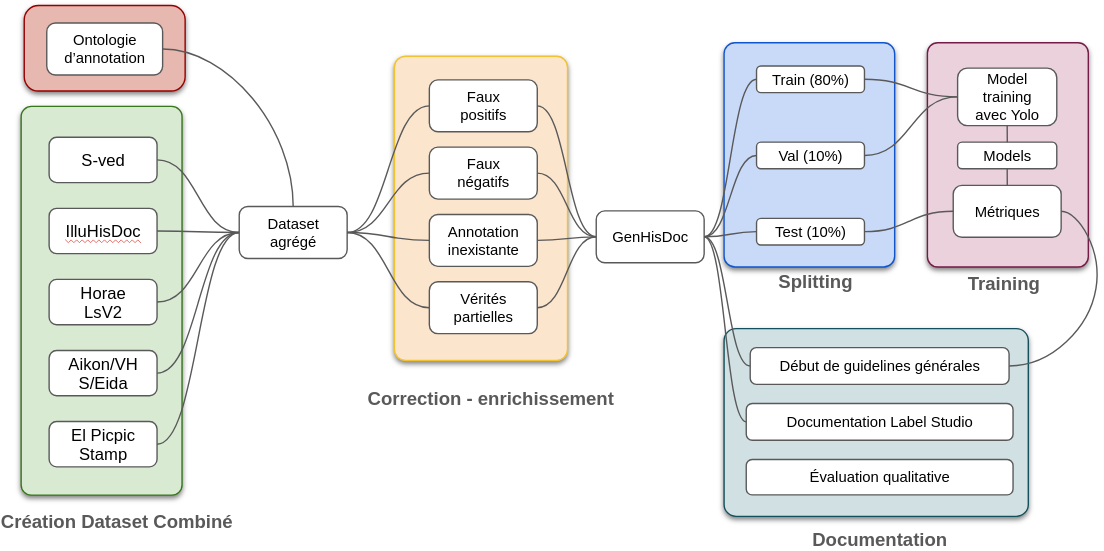
\includegraphics[scale=0.5]{img/GenHisDocOrganisation.png}
	\caption{Organisation du projet de stage et structuration des corpus dans GenHisDoc}
	\label{fig:GenHisDoc}
\end{figure}


C'est dans ce contexte qu'a eu lieu, entre début mai et fin juillet 2026, le stage au sein de l'équipe en charge du développement d'AIKON dans le laboratoire IMAGINE à l'\gls{enpc}. L'objectif principal était de construire un corpus d'entraînement de modèles de détection pour la plateforme. Pour arriver à cette fin, le travail a nécessité la définition d'une méthodologie préalable de constitution d'un corpus et de l'élaboration d'un vocabulaire d'annotation contrôlé en collaboration avec les projets \gls{vhs} et \gls{eida},  puis la construction d'un \textit{pipeline} d'entraînement d'un modèle de détection et de ses métriques pour l'évaluer. Plutôt que de constituer un jeu de données en partant de zéro, nous nous sommes intéressés à la question de la réutilisation et de la combinaison de travaux similaires dont les droits nous le permettaient. En plus de cette question de la réutilisation des matériaux de la recherche, nous nous sommes également intéressé à la capitalisation sur les matériaux d'annotation déjà produits par les utilisateurs d'AIKON. Réutiliser des données déjà annotées ajoute une couche de complexité à la constitution d'un jeu de données et nous avons exploré certaines stratégies de contournement, notamment pour les éléments comme les estampilles, pour diminuer l'effort d'annotation d'un élément relativement ignoré des jeux de données à visée patrimoniale.


Ce travail soulève une question : comment tous ces choix, qui impliquent une mise en données, conditionnent-t-ils l'efficacité de la vision par ordinateur dans le domaine de l'heuristique, c'est-à-dire la capacité à travailler sur un document historique et à en produire une analyse pertinente et scientifique ?

Dans un premier temps, nous dresserons un état de l'art de la rencontre entre vision par ordinateur et recherche historique. Nous retracerons d'abord l'évolution des technologies d'analyse d'images documentaires, depuis l'origine de la vision artificielle jusqu'à l'avènement des modèles vision-langage et des approches \textit{zero-shot}, en passant par les architectures \gls{yolo} et \gls{detr}. Nous analyserons ensuite la manière dont la communauté des historiennes et des historiens s'approprie ces outils, en observant les transformations de la pratique scientifique, la fabrique de la vérité de terrain et l'émergence d'une « nouvelle économie de l'érudition ». Enfin, nous situerons ce travail au sein de l'écosystème de la recherche en présentant le projet Aikon, ses objectifs scientifiques et ses réalisations techniques, tout en le confrontant aux autres initiatives nationales et internationales de vision artificielle historique.

Ensuite, nous détaillerons le processus de construction d'un corpus de numérisations adapté aux exigences de la vision artificielle. Nous traiterons d'abord des enjeux de la préparation d'une campagne d'annotation, qui nécessite de formaliser une ontologie appliquée aux documents historiques, de tracer des frontières sémantiques claires face aux cas limites et de rédiger des consignes rigoureuses. Nous expliciterons ensuite la constitution concrète du corpus, en abordant la réutilisation de jeux de données existants (tels que S-VED, IlluHisDoc ou Horae) et la récupération des métadonnées d'Aikon via \gls{iiif}, ainsi que les défis techniques liés à l'harmonisation des formats et à la correction des annotations sous Label Studio.

Enfin, nous analyserons l'entraînement et l'évaluation du modèle entraîné sur notre jeu de données. Après avoir détaillé le rôle et l'impact des hyperparamètres sur la dynamique d'apprentissage, nous présenterons la méthodologie d'évaluation mise en œuvre et analyserons les résultats obtenus sur la détection des différentes catégories d'objets (illustrations, ornements, lettrines, tampons et tables). Pour finir, nous confronterons ces métriques aux limites observées afin de dégager des pistes d'amélioration ciblées, qu'il s'agisse de l'ajustement des paramètres, du perfectionnement du protocole d'évaluation, du raffinage des annotations ou d'une refonte de l'ontologie.
















\newpage{\pagestyle{empty}\cleardoublepage}

%%%%%%%%%%%%%%%%%Le corps du mémoire
	\mainmatter

\part{La vision par ordinateur et l’historien : rétrospective, enjeux et méthodes}


\section*{Introduction}
\sectionmark{Introduction}


\begin{quote}
    \textit{Dans l'état actuel des connaissances en sémiologie, l'image apparaît comme un univers à la complexité redoutable : ses lois sont mal connues. Cela par opposition à la parole linguistique, qui semble plus accessible, mieux apprivoisée... Or l'une et l'autre apparaissent souvent ensemble [...] et parfois étroitement mêlées}\vspace{0.2cm}
    
    Laurence Badin, \og  Le texte et l'image \fg, dans \textit{Communication \& Langages}, vol 26, pp. 98-112 , 1975
\end{quote}

\lettrine{L}{'application de méthodes} informatiques sur les sujets de sciences humaines et sociales a toujours une forme de bricolage. Comme souvent, le chercheur se retrouve à utiliser des outils qui n'ont pas été pensés pour sa discipline et se doit de les réadapter pour sa pratique scientifique ; le domaine de la vision artificielle ne fait pas exception. Dans cette partie, nous nous intéresserons aux modes de développement et au fonctionnement de l'écosystème international des technologies que nous essayons de réadapter à des questions historiques. 

D'abord, nous contextualiserons ce qu'est la vision artificielle et les différentes phases techniques et conceptuelles par lesquelles la discipline s'est formée pour en arriver aux technologies actuelles applicables à des documents historiques. Ensuite, nous étudierons les différents tests, déploiements et expériences de l'utilisation de la vision artificielle dans le domaine de l'étude du document et des institutions patrimoniales. Enfin, nous nous concentrerons sur une réflexion historienne sur la place de ces outils en fonction des différents besoins de recherche. 
\chapter[L'émergence du traitement d'images historiques]{Le traitement et l'analyse automatique de documents : comment s'est construit l'écosystème technique puis scientifique actuel.}


\lettrine{L}{'image}, à l'instar d'un document sonore ou d'une œuvre plastique, est par essence silencieuse : elle ne s'exprime que par sa propre matérialité. Aucune description, aussi minutieuse soit-elle, ne saurait véritablement se substituer à son appréhension visuelle. Pourtant, la nécessité de décrire, d'indexer et de classer ces documents non textuels s'est imposée aux professionnels du patrimoine (bibliothécaires, archivistes) bien avant l'ère des catalogues informatiques et des instruments de recherche numériques. Face à ce défi descriptif, l'idée de traiter automatiquement une image par l'analyse de ses seules caractéristiques intrinsèques, sans recourir à des métadonnées externes, est dès les origines l'une des quêtes principale de la recherche en vision artificielle\footnote{Michael Brady, \og Intelligent Vision \fg, dans \textit{AI in the 1980s and Beyond}, éditions The MIT Press, 1989}.

\section[L'origine de la vision documentaire]{Les \gls{cnn} appliqués à la vision : une technologie ancienne}

Le domaine de la vision artificielle est aussi vaste qu'un \oe il peut être utile. Il est cependant important de connaître les tâches de base, les problématiques intrinsèques de la discipline car elles en forment les contours, et donc les limites avec lesquelles doit composer le domaine des humanités. 

\subsection{La naissance de la vision artificielle appliquée aux documents}

Très fortement lié à l'imitation des capacités cognitives humaines, l'acte de naissance du \textit{machine learning} trouve sa source dans le développement du neurone algorithmique\footnote{Warren S. McCulloch \& Walter Pitts, \og A Logical Calculus of the Ideas Immanent in Nervous Activity \fg, dans \textit{The bulletin of mathematical biophysics}, Vol 5, pp. 115–133, 1943}, puis dans les travaux d'optimisation statistique. C'est avec ce principe skeuomorphique que Kunihiko Fukushima crée en 1975 le principe des réseaux de neurones convolutifs, en s'inspirant du fonctionnement du cortex visuel. Ce principe initial sera ensuite amélioré par la technique de la \og rétro-propagation du gradient \fg, découverte plus ou moins simultanément en 1985 par au moins trois équipes différentes. 


L'une des premières applications de technologies de vision à l'analyse de documents est la reconnaissance optique de caractères manuscrits pour le domaine postal et bancaire, notamment par le modèle \textit{LeNet} mis au point par \textit{AT\&T Bell Laboratories} autour de la figure de Yann LeCun entre 1988 et 1998. Avant même les bibliothèques, les archives, et les laboratoires en sciences humaines, c'est dans les industries administratives (services postaux, banques) que la vision artificielle et l'analyse automatique de documents trouvent une première application concrète notamment dans la lecture de numéros de chèques et de codes postaux. \textit{LeNet} est également l'acte de naissance de l'apprentissage profond.

\subsection{La mise en place de la vision dans les institutions patrimoniales françaises}

L'utilisation de la vision artificielle à la \gls{bnf} se concentre d'abord sur le texte et l'\gls{ocr} notamment avec l'introduction du mode texte dans Gallica à partir de 2005 et du \textit{projet d'Analyse des résultats par \gls{ocr} des documents numérisés de la \gls{bnf}} par Kamel Ait-Mohand\footnote{Kamel Ait-Mohand, \og Techniques d'adaptation de modèles markoviens. Application à la reconnaissance de documents anciens\fg, Thèse de doctorat dirigé par Thierry Paquet , soutenance en 2011.} en 2008. Concernant le travail sur l'image historique et l'iconographie, les institutions patrimoniales se concentrent principalement sur des projets d'indexations et de correspondances de thésaurus comme en 2003 avec la mise en ligne de la base \textit{Mandragore} alors existante depuis 1989\footnote{Jean-Pierre Aniel, \og MANDRAGORE . Une base de données iconographiques sur les manuscrits de la \gls{bnf} \fg, dans \textit{Le médiéviste et l'ordinateur}, n°26-27, p. 18-20, 1992-1993}, ou en 2006 du projet \gls{stich}\footnote{\og STITCH : Semantic Interoperability to Access Cultural Heritage\fg , URL \href{https://actions-recherche.bnf.fr/bnf/anirw3.nsf/IX01/A2014000409\_stitch-semantic-interoperability-to-access-cultural-heritage?opendocument\&n=1\&categorie=2006}{lien vers la page action recherche}} à la \gls{bnf}. 

\subsection{2005-2010 : la prise de conscience de l'importance des données}
La décennie 2000 est également synonyme d'un changement de paradigme grâce à deux innovations. D'abord, c'est à partir de 2005 qu'il est démontré de l'intérêt de déporter les calculs d'un \gls{cnn} du processeur à une carte graphique\footnote{Dave Steinkrau, Patrice Y. Simard, Ian Buck, \og Using GPUs for Machine Learning Algorithms \fg, dans \textit{Eighth International Conference on Document Analysis and Recognition (ICDAR)}, pp.1115-1119, 2005}. Ensuite, c'est en 2006 que Fei Fei Li, une informaticienne d'origine chinoise de l'université de Standford, théorise que l'innovation dans les modèles de vision n'est pas suffisante pour améliorer leurs performances et qu'il faut alors produire des données de meilleure qualité ; ce qu'elle met en pratique en créant le jeu de données \textit{ImageNet}\footnote{J. Deng, W. Dong, R. Socher, L. -J. Li, Kai Li and Li Fei-Fei, \og ImageNet: A large-scale hierarchical image database\fg, dans \textit{2009 IEEE Conference on Computer Vision and Pattern Recognition}, Miami, FL, USA, pp. 248-255, 2009, doi: 10.1109/CVPR.2009.5206848.} en 2009 et de sa compétition associé, l'\gls{ilsvrc} un an plus tard. C'est ce tournant de 2009, passant d'une réflexion uniquement portée sur l'architecture de l'algorithme à la prise de conscience de l'importance dans la qualité et de la méthodologie de sélection des données d'entraînement qui fait entrer la vision artificielle dans sa période de maturité technologique.

\section[La vision aujourd'hui]{La décennie 2010 : le tournant des \gls{rcnn}}

Parmi ces jeux de données publiés chaque années à l'occasion de compétition, l'un des plus importants a été le dataset \textit{PASCAL VOC}. Cette compétition de détection tenue chaque année entre 2005 et 2012 démontrait que l'architecture des réseaux convolutifs devenait plus complexe mais tout en atteignant un plateau de performance. C'est en 2013 qu'est dévoilée la première architecture de réseaux à extraction de région\footnote{R. Girshick, J. Donahue, T. Darrell et J. Malik, \og Region-Based Convolutional Networks for Accurate Object Detection and Segmentation\fg dans \textit{IEEE Transactions on Pattern Analysis and Machine Intelligence}, vol. 38, no. 1, pp. 142-158, 2016, doi: 10.1109/TPAMI.2015.2437384.} \gls{rcnn} qui a l'avantage de grandement simplifier l'architecture du modèle tout en dépassant les plafonds des anciennes itérations.


Ce sont des modèles spécialisés dans la détection de région dans des images (détection, segmentation), les rendant rapidement irremplaçables dans les utilisations appliquées aux documents historiques. Le principe d'un \gls{rcnn} c'est l'application d'un pré-traitement à l'image avant d'utiliser un \gls{cnn} classique. L'opération de pré-traitement regroupe les pixels de l'image au sein d'une représentation en graphes\footnote{Lilian Weng, \og Object Detection for Dummies Part I : Gradient Vector, HOG, and SS \fg, sur \href{https:\/\/lilianweng.github.io\/posts\/2017-10-29-object-recognition-part-1\/}{lilianweng.github.io}} puis de prédire une probabilité de présence d'un objet par rapport à un fond grâce à un algorithme nommé \textit{algorithme de recherche sélective}\footnote{Pedro F. Felzenswalb, Daniel P. Huttenlocher, \og Efficient Graph-Based Image Segmentation \fg, dans \textit{International Journal of Computer Vision}, n°59, vol 2, pp.167–181, 2004}.


    \begin{figure}
        \centering
        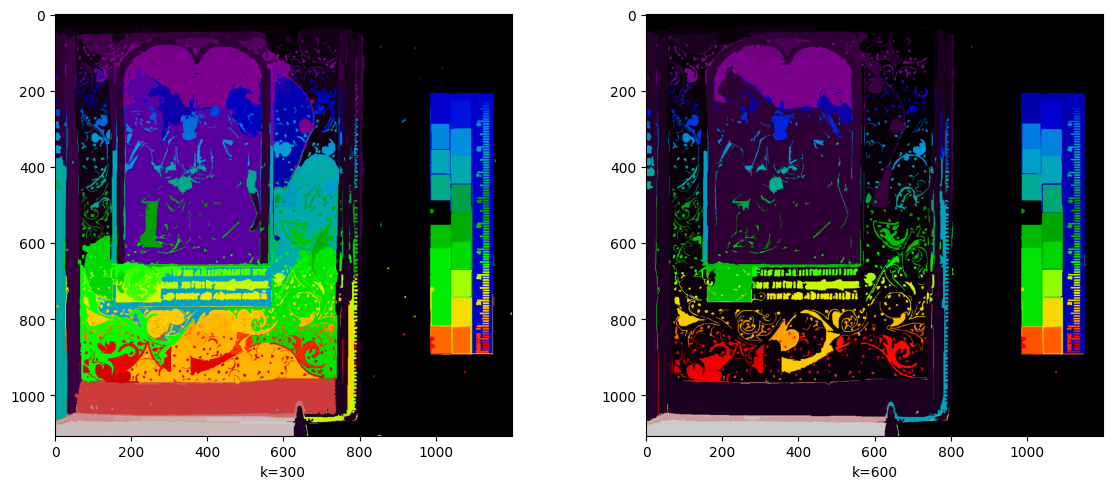
\includegraphics[scale=0.4]{img/felzenszwalb.png}
        \caption{Application d'une segmentation Felzenszwalb à une page d'un livre d'heure du dataset Horae LSv2. Premièrement avec une segmentation fine avec un seuil de tolérance bas (k=300), et un seuil de tolérance haut (k=600). Le seuil de tolérance détermine à quel point deux zones voisines doivent être différentes pour que l'algorithme refuse de les fusionner et décide de tracer une frontière entre elles.}
        \label{fig:felzenszwalb}
    \end{figure}


Rapidement, les travaux sur les modèles \gls{rcnn} vont mener à la création de sous-familles plus perfomantes comme Fast R-CNN\footnote{Ross Girshick, \og Fast R-CNN \fg, communication pour l'\textit{International Conference on  Computer Vision 2015}, 2015, URL: \href{  	
https://doi.org/10.48550/arXiv.1504.08083}{  	
https://doi.org/10.48550/arXiv.1504.08083}} pour la détection d'objets, puis Faster R-CNN qui améliore encore la performance des modèles ou Mask R-CNN qui étend les avancées de Faster R-CNN à la segmentation par pixel. 

\subsection{\textit{You Only Look Once} (\gls{yolo})}

Dans le domaine patrimonial, ces avancées se sont traduites par une meilleure performance dans la capacité des modèles à traiter des documents patrimoniaux, mais également la possibilité d'utiliser plusieurs méthodologies plus ou moins complexes. Le programme-cadre (framework) le plus populaire pour une utilisation patrimoniale est la famille des modèles \gls{yolo}  introduite par Joseph Redmon\footnote{J. Redmon, A. Farhadi, \og YOLO \fg, communication pour \textit{2016 Computer Vision and Pattern Recognition Conference}, 2016} puis amélioré à partir de la version 4 par plusieurs chercheurs, institutions et entreprises. Sa popularité tient du fait que le modèle ne fait qu'une seule proposition de région (rétro-propagation) avant d'effectuer ses prédictions, contrairement aux autres architectures de \gls{rcnn} qui peuvent répéter cette étape de rétro-propagation plusieurs milliers de fois par image. 

Les modèles de détection d'AIKON sont actuellement deux \gls{yolo} version 5\footnote{Ségolène Albouy, URL : \href{https://huggingface.co/seglinglin/Historical-Illustration-Extraction/tree/main}{sur Huggin Face}} (un pour les illustrations et un pour les diagrammes) et nous avons entraîné durant le stage un \gls{yolo} version 8 et un \gls{yolo} version 26\footnote{Jules Musquin, URL : \href{https://huggingface.co/Anarchiviste/GenHisDoc_model}{https://huggingface.co/Anarchiviste/GenHisDoc\_model}}.  AIKON utilise également d'autres types de modèles comme un Faster-RCNN pour la détection de filigranes ou la détection de lignes de texte. Aujourd'hui \gls{yolo} ne réfère plus réellement à une famille de modèles précis mais à un concept général d'architecture. Si les principaux modèles sont publiés et maintenus en open source, la bibliothèque python la plus utilisée est celle de l'entreprise \textit{Ultralytics}, critiquée pour sa tendance à s'approprier le projet \gls{yolo} qui était à la base open-source. \textit{Tiamat}, un projet similaire relativement similaire à AIKON, porté par le consortium \textit{HN-Humanum Pictoria} utilise également cette architecture \gls{yolo}\footnote{Fantin Le Ber \og IA et patrimoine, un changement dans la continuité : l’exemple du projet Highvision\fg, mémoire de master, \textit{École nationale des chartes}, 2025}. 


\subsection{\gls{detr} : le concurrent direct de \gls{yolo}}

En 2020, l'entreprise Facebook, aujourd'hui renommée Meta, dévoile l'architecture \gls{detr} qui combine une base convolutive \gls{resnet} avec un \textit{transformer} (attention globale). Si les architectures \gls{detr} ne sont pas encore énormément utilisées en production dans les institutions patrimoniales, ces modèles récupère des parts de marché. Cette avantage grandit pour deux raisons principales : 
\begin{description}
    \item \textbf{La licence d'exploitation} : La licence des modèles \gls{yolo} publiés par \textit{Ultralytics} est au format \gls{agpl}-3.0. L'utilisation est donc gratuite seulement si le projet est lui-même open-source ou l'institution doit payer une licence d'entreprise. Les modèles \gls{detr} et les environnements fournis par Meta sont aujourd'hui au format de licence Apache 2.0, autorisant une réutilisation privée ou commerciale gratuite.

    \item \textbf{Les gains de performance grầce à l'utilisation des \textit{transformers}} : \gls{detr} introduit dans la vision artificielle l'utilisation de la technologie \textit{transformers}\footnote{Ashish Vaswani, Noam Shazeer, Niki Parmar, Jakob Uszkoreit, Llion Jones, Aidan N. Gomez, Lukasz Kaiser, Illia Polosukhin, \og Attention is All You Need \fg, communication pour \textit{2017 Advances in Neural Information Processing Systems} (NIPS), 2017}. L'avantage principale de cette architecture étant l'efficacité de la parallélisation des calcules car un transformer ne demande pas un calcul séquentiel des données contrairement à un \gls{cnn}.  Dans cette nouvelle architecture, la détection de classes dans une image devient un opération d'ensemble directe (\textit{direct set prediction})\footnote{Nicolas Carion, Francisco Massa, Gabriel Synnaeve, Nicolas Usunier,
    Alexander Kirillov, Sergey Zagoruyko, \og End-to-End Object Detection with Transformers \fg, communication pour \textit{2020 European Conference on Computer Vision} (ECCV), 2020, DOI: \href{arXiv:2005.12872}{arXiv:2005.12872}}. Le programme utilise d'abord un \gls{cnn} qui permet d'extraire certaines informations de l'image, puis un couple encodeur-décodeur permettant d'extraire une prédiction pour les classes et une prédiction pour les boundings boxes\footnote{Yu Liang, Tang Lin, Mu Lisha, \og A Review of DEtection TRansformer: From Basic Architecture to Advanced Developments and Visual Perception Applications\fg, dans \textit{Sensors}, n°25, vol°13, 2025, DOI: \href{10.3390/s25133952}{10.3390/s25133952}}.
\end{description}

\section[2020 : les nouvelles approches]{La décennie 2020 : la maturité opérationnelle et l'apparition de nouvelles approches}. 

Dans le domaine de la vision, jusqu'aux \gls{rcnn} et \gls{yolo}, la détection n'était que géométrique : le modèle isolait des pixels (une boîte ou un masque) comme faisant partie d'une classe. Les chercheurs dès 2015 créent les premiers modèles de vision multimodaux combinant texte et image (\textit{image captioning systems}), ce sont des \gls{cnn} capable de générer des annotations au niveau de l'image\footnote{Kelvin Xu, Jimmy Ba, Ryan Kiros, Kyunghyun Cho, Aaron Courville, Ruslan Salakhutdinov, Richard Zemel, Yoshua Bengio, \og Show, Attend and Tell: Neural Image Caption Generation with Visual Attention\fg, publié sur ArXiv, DOI : \href{10.48550/arXiv.1502.03044}{10.48550/arXiv.1502.03044}}, et donc de faciliter les tâches de classifications. 

\subsection{Les \textit{Visual Language Models} (\gls{vlm}) : Du pixel à la sémantique}

À partir de 2018, cette approche multimodale va connaître une évolution rapide avec dans un premier temps l'application de la technologie des \textit{Transformers} qui sont fait pour le traitement du langage naturel et donc qui offrent des liens entre le texte et l'image bien plus profonds. Le domaine profite également de la création de nouveaux jeux de données d'entraînement généralisés comme \textit{MS COCO}\footnote{Tsung-Yi Lin,  Michael Maire, Serge Belongie, Lubomir Bourdev, Ross Girshick, James Hays, Pietro Perona, Deva Ramanan, C. Lawrence, Zitnick Piotr Dollar, \og Microsoft COCO: Common Objects in Context \fg, publié sur ArXiv, 2015, DOI: \href{arXiv:1405.0312v}{arXiv:1405.0312v}}, pourvoyant des annotations sous forme de paires d'images et de texte descriptif. Plusieurs nouveaux types de tâches apparaissent dans le sillage des évolutions comme le \gls{vqa} ou le \textit{Phrase Grounding} qui peut transformer un texte qui décrit une image en une référence spatialisée dans l'image avec des boîtes englobantes\footnote{Timothy M, \og What is Phrase Grounding \fg, post de blog sur Roboflow, 2024, URL : \href{https://blog.roboflow.com/what-is-phrase-grounding/}{Lien vers le blog}}.

En 2021, OpenIA rend public le premier modèle \gls{vlm} de fondation  avec  \textit{CLIP} (Contrastive Language–Image Pretraining). La capacité de traitement du texte d'un \gls{vlm}, et la montée en popularité des systèmes \gls{rag} fait que le milieu documentaire va rapidement s'imposer comme un sujet de choix pour l'application de ces technologies avec dès 2021 la mise à disposition par Microsoft de \textit{LayoutLM}\footnote{Yiheng Xu, Minghao Li, Lei Cui, Shaohan Huang, Furu Wei, Ming Zhou, \og LayoutLM: Pre-training of Text and Layout for Document Image Understanding \fg, communication pour \textit{26th ACM SIGKDD International Conference on Knowledge Discovery \& Data Mining}, 2020, DOI: \href{arXiv:1912.13318v5}{arXiv:1912.13318v5}},  un modèle permettant de joindre l'\gls{ocr} et la reconnaissance de mise en page dans des documents contemporains \gls{olr}. C'est cette articulation conjointe du visuel et du textuel qui ouvre une perspective inédite pour l'analyse de documents patrimoniaux en imitant l'humain en liant le contenu et le contenant\footnote{Sina Semnani, Han Zhang, Xinyan He, Merve Tekgurler, Monica Lam, \og CHURRO: Making History Readable with an Open-Weight Large Vision-Language Model for High-Accuracy, Low-Cost Historical Text Recognition\fg,}. 

Cependant il est intéressant de noté quelques limites à ces technologies que nous tirons d'un article de Maria Levchenko sur une méthodologie d'évaluation des VLM dans le contexte de la lecture de document historique\footnote{Maria Levchenko, \og Evaluating LLMs for Historical Document OCR: A Methodological Framework for Digital Humanities\fg, publié sur ArXiv, 2025, DOI : \href{arXiv:2510.06743v1}{arXiv:2510.06743v1}} que nous pouvons regrouper trois grands arguments. Premièrement, cette famille de modèle performent le mieux sur du texte imprimé Les testes entre VLM et R-CNN se font majoritairement sur des tâches d'OCR. Ces technologies performent le mieux dans des situations où d'autres technologies moins complexes performent également à un niveau acceptable. Cependant ils semblent présenter un avantage pour l'HTR, ou dans certaines conditions comme une mise en page difficile ou un document un peu trop abîmé\footnote{Seorin Kim , Julien Baudru, Wouter Ryckbosch, Hugues Bersini, Vincent Ginis, \og Early evidence of how LLMs outperform traditional systems on OCR/HTR tasks for historical records\fg, publié sur ArXiv, 2025, DOI : \href{arXiv:2501.11623v1}{arXiv:2501.11623v1}}. Ensuite, toutes les familles de modèles "génératifs" ont des comportements non-déterministes lors de différents passages d'un même document avec un même modèle\footnote{ Marie Puren, Donghan Bian, Aurélien Pellet, Julien Perez, Florian Cafiero, \og  Aligner méthode historique et RAG : transformer un
assistant conversationnel en chaîne de preuve auditable et
discutable\fg, communication pour \textit{Humanistica 2026, Association francophone des humanités numériques}, pp.1-9, 2026, DOI: \href{10.63744/G14mF7UizFzS }{10.63744/G14mF7UizFzS }}. Enfin, les VLM font partie des programmes les plus onéreux à faire tourner actuellement, que ce soit en terme de ressource machine (RAM, Calcule sur GPU, temps de calcule) ou en prix de déploiement chez un fournisseur. La question du passage d'un document dont la numérisation est potentiellement sous-droit dans un modèle qui n'est disponible que chez un fournisseur pose également une question de propriété intellectuelle.


\subsection{Les modèles fondateurs et l'apparition de l'approche \textit{Zero-shot} / \textit{Few-shot}}

Aujourd'hui, l'application de la vision par ordinateur aux sources historiques imposait aux chercheurs un véritable travail d'annotation sérielle. Les applications institutionnelles qui permettent l'utilisation de la vision pour public non technique dans le style d'Aikon permettent de mutualiser l'utilisation d'un modèle entre les utilisateurs et donc d'utiliser les outils plus complexes et entraînés sur plus de données. 

Pour entraîner un modèle à reconnaître détecter ou segmenter les éléments d'une page, il est indispensable de constituer \textit{ex nihilo} de volumineux jeux de données (des données que le modèle n'a jamais vu). Les équipes et les historien\pmm nes se voient ainsi contraint d'assumer le rôle de producteur de données, passant un temps considérable à tracer manuellement les annotations(\textit{bounding boxes}). 

L'émergence des modèles dits « fondateurs » (\textit{Foundation Models}) pourrait peut être rompre une partie de ce goulot d'étranglement. Pré-entraînés sur des volumes massifs d'images et de textes, des architectures multimodales comme \textit{Florence-2}\footnote{Bin Xiao, Haiping Wu, Weijian Xu, Xiyang Dai, Houdong Hu, Yumao Lu, Michael Zeng, Ce Liu, Lu Yuan, \og Florence-2: Advancing a Unified Representation for a Variety of Vision Tasks \fg, publié sur ArXiv, 2023, DOI: \href{https://arxiv.org/abs/2311.06242}{https://arxiv.org/abs/2311.06242}} ou les grands VLM généralistes disposent d'une représentation du monde visuel suffisante pour travailler sur un document historique sans entraînement préalable. Cette puissance leur permet dans certains cas de fonctionner selon deux modes inédits pour la vision patrimoniale : le \textit{Zero-shot}, capable d'exécuter une tâche de segmentation, de détection ou de description sans aucun entraînement préalable sur le corpus cible, et le \textit{Few-shot}, qui ne nécessite qu'un nombre très restreint d'exemples pour guider le modèle ou effectuer un réalignement léger (\textit{fine-tuning}).

Par exemple, après notre stage, nous avons notamment essayé d'aider Eva Rivière à faire tourner \textit{Florence-2} dans une tache d'annotation d'image de façade de bâtiments en  \textit{Zero-shot} de \textit{Phase Grounding}\footnote{Jules Musquin, Eva\_benchmark\_torne-h
 sur \href{https://github.com/Anarchiviste/Eva_benchmark_torne-h}{Github}} en offrant au modèle une image d'une façade et une description au format json des éléments à annoter. Si nous avons réussi à faire tourner un modèle aussi lourd sur nos équipements personnels, nous n'avons cependant pas réussi à sortir un image traitée correctement. Cette expérience rapide montre à la fois les espoirs que suscite cette capacité d'annotation zero-shot mais également les problèmes techniques de coût et de puissance de calcule de ces technologies. 

%L'idée forte : La décennie 2010 imposait à l'historien un travail de forçat : créer des datasets massifs (des milliers de bounding boxes) pour entraîner un modèle de zéro.

%Le basculement : L'arrivée des modèles pré-entraînés massifs (les Foundation Models comme Florence-2, SAM ou les grands LLM visuels) qui fonctionnent en Zero-shot (sans entraînement) ou avec très peu de données (Few-shot / Fine-tuning léger).

%yL'enjeu historique : Cela démocratise l'IA pour l'histoire. L'historien n'a plus besoin d'être un producteur industriel de données. L'acte de recherche se déplace : on passe de l'annotation de masse à l'ingénierie de la requête (le prompt) et au réglage fin sur des sources hyperspécifiques (ce que tu as fait avec GenHisDoc sur YOLO).




\chapter[Vision artificielle et humanités]{Vision artificielle et humanités : de la performance algorithmique à l'herméneutique des données}

\lettrine{L}{es} chercheurs et les institutions qui appliquent la vision artificielle aux corpus historiques se heurtent souvent à l'opacité technique de ces outils. Dès lors, la pertinence de ces technologies pour les humanités numériques ne se mesure pas à leur seule performance algorithmique, mais à la rigueur méthodologique avec laquelle elles s'articulent aux exigences d'une discipline et d'un programme de recherche spécifiques.

\section[La prise en main par les chercheurs]{La prise en main par les chercheurs : une dépendance technique et une divergence d'objectifs}

Le domaine des humanités et de l'analyse de documents n'utilise qu'une petite fraction des avancées du monde de la vision artificielle. La recherche et l'industrie informatique se concentrent aujourd'hui principalement sur d'autres problématiques comme la segmentation vidéo en temps réel ou la création de modèles génératifs multimodaux. De son côté, la vision patrimoniale se focalise sur une typologie de besoins bien précise : la classification, l'analyse de mise en page (layout analysis), la détection d'objets et, plus récemment la segmentation.

Ici sans prendre en compte les tầches d'\gls{ocr} et d'\gls{htr}, la vision artificielle appliquée aux corpus patrimoniaux s'articule autour de quatre tâches fondamentales dont la complexité et les coûts d'annotation varient sensiblement. 

\subsection{Les tâches la vision à visée patrimoniale}

\subsubsection{La classification globale} Elle vise à attribuer une étiquette unique à une image complète. Elle est adaptée à des tâches de tri relativement grossières qui, dans notre cadre, permettent le tri automatisé de grandes masses documentaires (distinction entre manuscrit et imprimé, identification du support, attribution du style d'une écriture). Son principale avantage vient d'un système d'annotation reposant sur une étiquette unique par image, et donc en utilisant également une ontologie simple.

\subsubsection{La détection d'objet et l'analyse de mise en page}
    
\begin{description}
    
    \item \textbf{La détection d'objets :} Reposant sur la délimitation par boîtes englobantes (\textit{bounding boxes}), elle permet de localiser et de catégoriser des entités visuelles discrètes au sein de la page. C'est l'outil privilégié des historiens de l'art et des codicologues pour repérer rapidement des lettrines, des sceaux, des filigranes ou des motifs iconographiques récurrents. Dans le projet AIKON, deux modèles de détection d'objets sont utilisés, un modèle de détection de diagramme et un modèle de détection d'illustration. Durant notre stage, l'une des stratégies que nous avons adoptées a été de rendre nos classes \og asémantiques\fg, c'est-à-dire de regrouper des éléments différents (illustrations ou diagrammes par exemple) sous une même bannière en dépit du sens dans le document pour privilégier une méthode d'annotation économique en temps et en moyens comme le montre l'image~\ref{fig:détection}. Bien plus coûteux que l'annotation d'une classification globale, le coût et la complexité de l'annotation pour l'analyse de mise en page dépendent des documents étudiés\footnote{Voir les grilles tarifaires moyennes des prestataires de labellisation de données (\textit{Data Annotation Pricing Guides}, 2025-2026 par DataVLab, Mindkosh AI et AI Superior) : le coût moyen d'une \textit{bounding box} varie entre 0,03 \$ et 0,08 \$ par objet, contre 0,50 \$ à 3,00 \$ par image pour une segmentation au pixel, traduisant un rapport de coût de 1 à 10 selon la complexité visuelle du document.}. 
    
    \item \textbf{L'analyse de mise en page (\textit{layout analysis}) :} C'est une sous-catégorie de la détection d'objets et une étape préalable indispensable à la lecture automatisée. Elle consiste à décomposer l'espace de la page pour en extraire la structure architecturale. Il s'agit d'isoler les blocs de texte principal, les gloses marginales, les colonnes, les en-têtes et les zones non textuelles afin de préserver l'ordre de lecture originel du document. Contrairement à la détection d'objets simple, les annotations sont donc divisées selon un sens de la mise en page et de la hiérarchie entre les éléments comme le montre l'image~\ref{fig:segmentation}. C'est l'une des formes d'annotations les plus coûteuses et les plus difficiles à mettre en œuvre, notamment à cause de la hiérarchie interclasse et de la relation entre les objets. La presse concentre la majorité des efforts car c'est l'un des domaines où la mise en page est complexe et coûteuse à annoter\footnote{ Benjamin Charles Germain Lee, Jaime Mears, Eileen Jakeway, Meghan Ferriter, Chris Adams, Nathan Yarasavage, Deborah Thomas, Kate Zwaard, Daniel S. Weld, \og The Newspaper Navigator Dataset: Extracting And Analyzing Visual Content from 16 Million Historic Newspaper Pages in Chronicling America\fg, publié sur ArXiv, 2020, URL : \href{https://arxiv.org/abs/2005.01583}{https://arxiv.org/abs/2005.01583}}. 
    
\end{description}
    
    %Bounding boxes: $0.02-$0.10 per object
    %Polygon annotations: $0.04-$0.15 per object
    %Semantic segmentation: $0.10-$3.00 per mask
    %3D point cloud labeling: $0.50-$5.00 per frame

\begin{figure}[htbp]
        \centering
        \begin{subfigure}{0.48\textwidth}
            \centering
            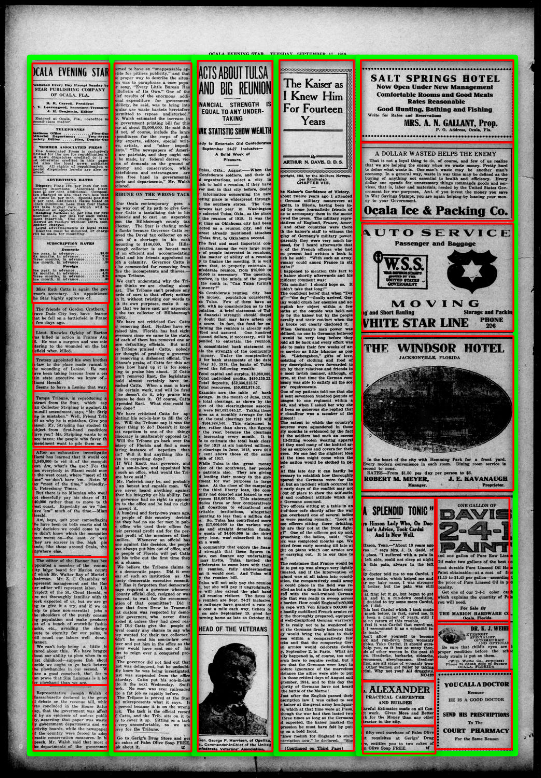
\includegraphics[scale=0.4]{img/segmentation.png}
            \caption{\textbf{Analyse de mise en page :} Exemple d'analyse simple de la mise en page d'une page de presse avec en vert les colonnes, et en rouge la segmentation des articles.}
            \label{fig:segmentation}
        \end{subfigure}
        \hfill
        \begin{subfigure}{0.48\textwidth}
            \centering
            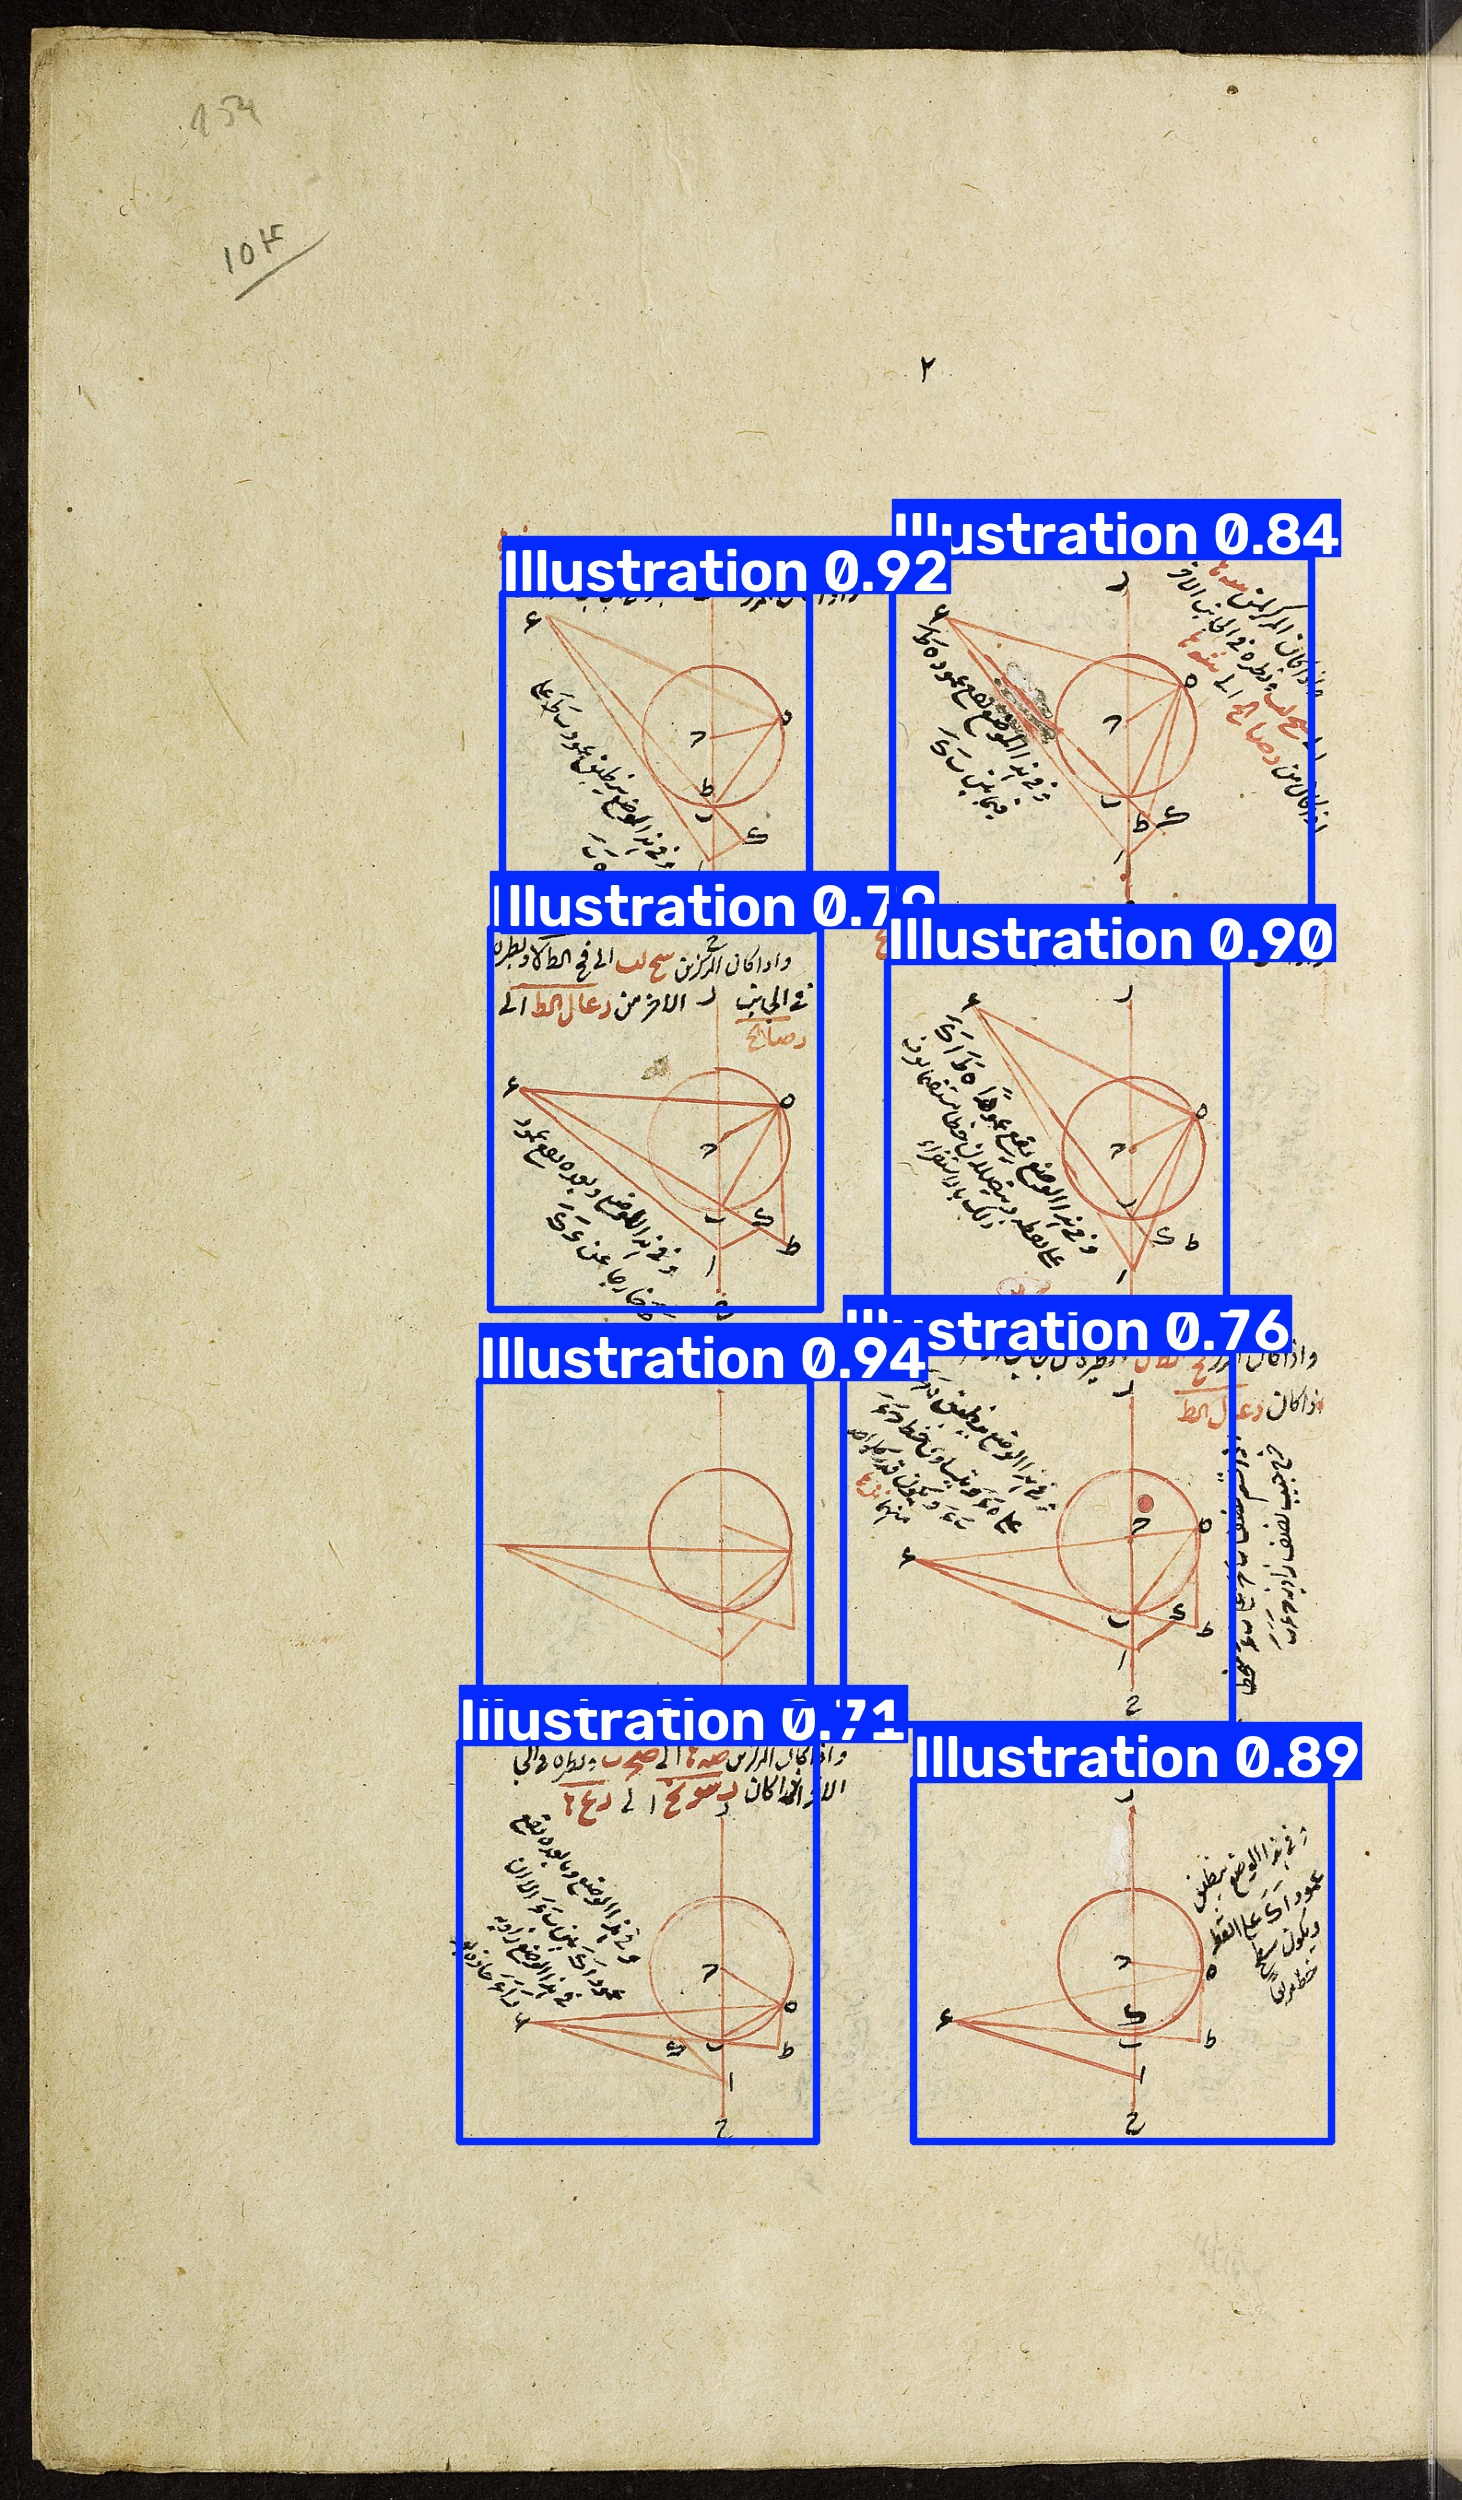
\includegraphics[scale=0.09]{img/detection.jpg}
            \caption{\textbf{Détection d'objets :} Exemple de détection produite par un modèle entraîné sur GenHisDoc. Ici le modèle détecte des illustrations sans hiérarchie ni organisation.}
            \label{fig:détection}
        \end{subfigure}
        \caption{Exemple de différence entre l'analyse de mise en page et la simple détection d'éléments dans la page.}
\end{figure}
    
\subsubsection{La segmentation au pixel :} Plus fine mais nettement plus coûteuses en annotation, la segmentation opère en attribuant une classe à chaque pixel de l'image comme montré dans la figure~\ref{fig:segexemple}. En vision patrimoniale, elle intervient principalement pour l'extraction de précision, qu'il s'agisse de tracer la ligne d'écriture exacte (\textit{baseline}) indispensable aux moteurs \gls{htr}, de détourer le fond d'un document dégradé ou d'isoler les contours complexes d'illustrations. La segmentation est l'une des pratiques les plus coûteuse, cependant c'est également un domaine très actif où des innovations comme \gls{sam}, un modèle rendu public par \textit{Meta} en 2023, permettent de transformer une détection en segmentation à un coût réduit\footnote{Alexander Kirillov, Eric Mintun, Nikhila Ravi, Hanzi Mao, Chloe Rolland, Laura Gustafson, Tete Xiao, Spencer Whitehead, Alexander C. Berg, Wan-Yen Lo, Piotr Dollár, Ross Girshick, \og Segment Anything \fg, publié sur ArXiv, URL : \href{https://arxiv.org/abs/2304.02643}{arXiv:2304.02643}}.

\subsection[Le triptyque Dataset / Modèle / Papier]{Le triptyque Dataset / Modèle / Papier, la compétition et les méthodes de mesure de performance biaisées qui en résultent.} 

Comme rappelé en introduction, le secteur de la vision artificielle appliquée aux documents s'est structuré autour d'un cycle de conférences avec des communications et compétitions internationales, à l'instar d'\gls{icdar} et d'\gls{icfhr}. Ces compétitions générales dépassent le seul cadre des applications aux corpus patrimoniaux et cela joue sur la manière dont le champ de recherche s'évalue et progresse. La publication d'un jeu de données donne alors lieu à l'entraînement d'un modèle de vision dont les performances seront validées par un article scientifique avec des métriques quantitatives. Cette focalisation sur la performance d'un modèle aide à choisir le meilleur outil pour réaliser une tâche de vision, mais n'est pas une bonne manière d'évaluer la scientificité d'un travail historique. L'acte méthodologique --- historiographique --- d'un projet de vision sur des documents patrimoniaux repose en réalité sur la construction de son ontologie d'annotation et la sur manière dont son jeu de données d'entraînement a été construit. 

% insérer une définition des métriques
\subsubsection{Les métriques de performances de base pour évaluer un modèle}

\begin{description}
    
        \item \textbf{Ground Truth (GT) / Vérité de terrain : }Le nombre total d'éléments d'intérêt (illustrations, schémas, etc.) réellement annotés à la main au sein du jeu de données de test. Il constitue la vérité de terrain de référence que le modèle cherche à retrouver.

        \item \textbf{Vrais Positifs (TP - \textit{True Positives}) :} Le nombre d'illustrations réelles correctement localisées et identifiées par le modèle.

        \item \textbf{Faux Positifs (FP - \textit{False Positives}) :} Le nombre d'erreurs par sur-détection. Il s'agit des cas où le modèle a prédit une illustration là où il n'y en avait pas (ex. une tache, un bloc de texte ou un élément d'ornementation non annoté).

        \item \textbf{Faux Négatifs (FN - \textit{False Negatives}) :} Le nombre d'omissions. Il représente les illustrations présentes dans les documents mais ignorées par le modèle.
    
\end{description}
    
\subsubsection{Les métriques de performance calculées pour évaluer un modèle:}

    \begin{description}
    
        \item \textbf{IoU Moyen (\textit{Intersection over Union}) :} L'indicateur de précision spatiale du tracé. L'IoU mesure le taux de recouvrement entre la boîte englobante prédite par le modèle ($B_p$) et la boîte réelle de la vérité de terrain ($B_{gt}$) :
        \begin{equation*}
            \text{IoU} = \frac{\text{Aire}(B_p \cap B_{gt})}{\text{Aire}(B_p \cup B_{gt})}
        \end{equation*}
        Plus l'IoU est élevé (ex. $> 0{,}85$), plus la localisation géométrique des boîtes englobantes est bonne. Cependant, l'IoU moyen mesure la qualité du tracé géométrique uniquement quand il y a un chevauchement entre une prédiction et une vérité terrain, et donc c'est une métrique masquant ainsi les faux négatifs (FN) et les faux positifs (FP). 

        \item \textbf{AP@50 / mAP@50 (\textit{La précision moyenne} (Average Precision) / \textit{mean Average Precision}) :} La métrique de référence en détection d'objets. Le seuil \texttt{@50} indique qu'une détection est considérée comme valide si son IoU avec la vérité de terrain est supérieur ou égal à $0{,}50$. L'AP calcule l'aire sous la courbe Précision/Rappel en balayant tous les seuils de confiance possibles (de $0$ à $1$), fournissant une évaluation globale de la capacité du modèle indépendamment d'un réglage particulier.
        
        l'AP porte sur une seule classe spécifique : C'est la Précision Moyenne calculée pour une seule catégorie d'objets.
        
        La mAP porte sur l'ensemble des classes détectées : Elle correspond à la moyenne des AP50 calculée sur l'ensemble des classes du jeu de données.

        \item \textbf{Précision :} La proportion de détections correctes parmi l'ensemble des prédictions effectuées par le modèle à un seuil de confiance donné :
        \begin{equation*}
            \text{Précision} = \frac{\text{Instances pertinentes récupérées (TP)}}{\text{Toutes les instances récupérées (TP + FP)}}
        \end{equation*}
        Dans le cadre de l'analyse automatique de documents, une précision élevée indique que presque tout ce que le modèle identifie comme étant un élément cible l'est réellement. Une précision élevée garantit à l'utilisateur que les boîtes générées contiennent très peu de faux bruit.

        \item \textbf{Rappel (\textit{Recall}) :} La proportion d'illustrations réellement retrouvées par le modèle par rapport au total des illustrations présentes dans le corpus :
        \begin{equation*}
            \text{Rappel} = \frac{\text{Instances pertinentes récupérées (TP)}}{\text{Toutes les instances pertinentes récupérées (TP + FN)}}
        \end{equation*}
        Pour une étude sérielle ou un inventaire, l'historien recherche l'exhaustivité. Il est souvent préférable d'avoir un modèle qui génère un peu de \og bruit \fg{} (Faux Positifs) que l'on éliminera rapidement à l'œil nu, plutôt qu'un modèle trop prudent qui omet des occurrences rares (Faux Négatifs). Un rappel élevé indique que le modèle ne rate presque aucune illustration dans un document.

        \item \textbf{Score F1 :} C'est la moyenne harmonique (moyenne entre des ratios, des taux ou des proportions) entre la Précision et le Rappel :
        \begin{equation*}
            \text{F1} = 2 \times \frac{\text{Précision} \times \text{Rappel}}{\text{Précision} + \text{Rappel}}
        \end{equation*}
        Il offre une mesure synthétique équilibrée du compromis entre exhaustivité (Rappel) et pertinence (Précision) à un seuil opérationnel fixe (ex. $\text{Conf} \ge 0{,}25$ ou $0{,}50$). Le Score F1 calculé à un seuil de confiance fixe est la métrique la plus pragmatique : elle indique l'équilibre réel entre exhaustivité et exactitude lors du déploiement du modèle sur un corpus de travail.
\end{description}

Dans le cadre des travaux menés sur le projet AIKON où nous travaillons sur la détection d'objets dans des documents, les trois métriques les plus pertinentes sont \textbf{le Rappel}, \textbf{la Précision} et \textbf{le Score F1}. Cependant pour d'autres tâches comme la segmentation de ligne d'écriture (\textit{Baseline Detection}), certaines métriques comme l'\textbf{Intersection over Union} à un seuil très discriminant (ex. $\text{Chevauchement} \ge 0{,}90$) deviennent primordiales pour éviter de mélanger les lignes d'écriture entre elles. Dans un projet visant à alimenter automatiquement une base de données iconographique, l'absence de bruit est privilégiée (pas de FP) et donc une précision élevée par rapport à son rappel ; inversement, lors d'une opération de dépouillement ou d'inventaire systématique des illustrations d'un manuscrit, le chercheur vise l'exhaustivité (absence de faux négatifs), ce qui exige un rappel élevé par rapport à la précision.

\section[De la prédiction à la connaissance]{De la prédiction géométrique à la connaissance historique : post-traitement, interprétation et structuration des résultats}

Dans le premier chapitre, nous avions vu que jusqu'aux alentours de 2010 s'affrontaient deux paradigmes. Le \textit{paradigme centré sur le modèle}, où l'amélioration technique amène à de meilleures performances, et le \textit{le paradigme centré sur la qualité des données}, où la qualité, la quantité et la diversité des données d'entraînement qui permettent de passer au-delà des impasses de l'approche centrée sur le modèle. Cependant, dans la partie précédente, nous avons conclu que pour une utilisation érudite comme en sciences historiques, la scientificité de l'utilisation de la vision artificielle passait d'abord par l'acte méthodologique de construction de l'ontologie d'annotation et de la manière dont les annotations sont conduites. En effet, le modèle n'apprend pas à \og voir \fg le document ou l'œuvre de manière neutre, il apprend à reproduire la grille de lecture définie par le schéma d'annotation sur de nouvelles images\footnote{Johannes Jakubik, Michael Vössing, Niklas Kühl, Jannis Walk, Gerhard Satzger, \og Data-Centric Artificial Intelligence \fg, publié sur ArXiv et accepté pour publication dans \textit{Business \& Information Systems Engineering}, pp.507–515, 2024, DOI: \href{https://arxiv.org/abs/2212.11854v4}{arXiv:2212.11854v4}}. À architecture égale, c'est la qualité des données qui produit la majorité des gains de performances et de possibilités d'utilisations. 

\subsection[La fabrique de la vérité de terrain]{La fabrique de la vérité de terrain (\textit{Ground Truth}) : L'importance de faire perdurer un écosystème de la vision patrimoniale}

Le but scientifique d'AIKON et de ses projets partenaires est d'étudier les méthodes d'interaction possibles entre un environnement technique et des spécialistes. Cela permet de produire de grands volumes de données de qualité de manière semi-automatique. Cependant, dans l'objectif de réutiliser ces données, de les mettre à disposition et de mettre en place un cercle vertueux d'amélioration continue de l'outil grâce aux résultats produits, il faut pouvoir superviser la grille de lecture qui lui est appliquée. Une bonne ontologie d'annotation permet à la fois de couper court à la majorité des ambiguïtés pour les annotateurs humains et de réduire le travail de correction en sortie de détection.

\subsubsection{Le découplage indispensable entre la structure physique et la  fonction sémantique}

La plupart des vocabulaires contrôlés utilisés comportent en moyenne cinq à six classes, avec un maximum autour d'une douzaine. L'une des erreurs méthodologiques majeures que l'on retrouve dans les jeux de données pour l'analyse de documents historiques consiste à mélanger la description visuelle et l'interprétation fonctionnelle. Dans la plupart des cas, les classes proposées sont mal adaptées aux documents historiques et, généralement, le vocabulaire utilisé ne sépare pas strictement l'analyse visuelle de la mise en page et la fonction textuelle ou sémantique. Nous notons également, dans la majorité des jeux de données historiques, l'absence des données tabulaires et des estampilles au sein des ontologies proposées.

Par exemple, le dataset S-VED\footnote{Jochen Büttner, Julius Martinetz, Hassan El-Hajj, Matteo Valleriani, \og CorDeep and the Sacrobosco Dataset: Detection of Visual Elements in Historical Documents \fg, dans \textit{Journal of Imaging}, pp.~285-303, 2022} propose une ontologie relativement simple constituée de quatre classes :
\begin{itemize}
	\item \textit{Illustration}
	\item \textit{Lettrine}
	\item \textit{Ornementation}
	\item \textit{Marque d'imprimeur}
\end{itemize}

\textit{Illustration}, \textit{Lettrine} et \textit{Ornementation} décrivent des éléments asémantiques (on ne fait pas de différence entre les types d'illustrations) et généraux (ces trois classes peuvent être utilisées sur des manuscrits comme sur des imprimés). Cependant, la classe \textit{Marque d'imprimeur} porte à la fois une information visuelle (une illustration) et sémantique (l'information véhiculée par l'illustration). De plus, les marques d'imprimeur constituent une spécificité propre aux livres imprimés, ce qui limite la réutilisation directe de l'ontologie du dataset S-VED ou exige un travail de correction sur les données. Attention, il est important de comprendre que le non-respect de ces règles ne rend pas un jeu de données inutile ou mauvais, mais il sera forcément plus difficile de le traiter et de le croiser avec d'autres jeux de données s'il ne se conforme pas à ces principes.

\begin{figure}[htbp]
	\centering
	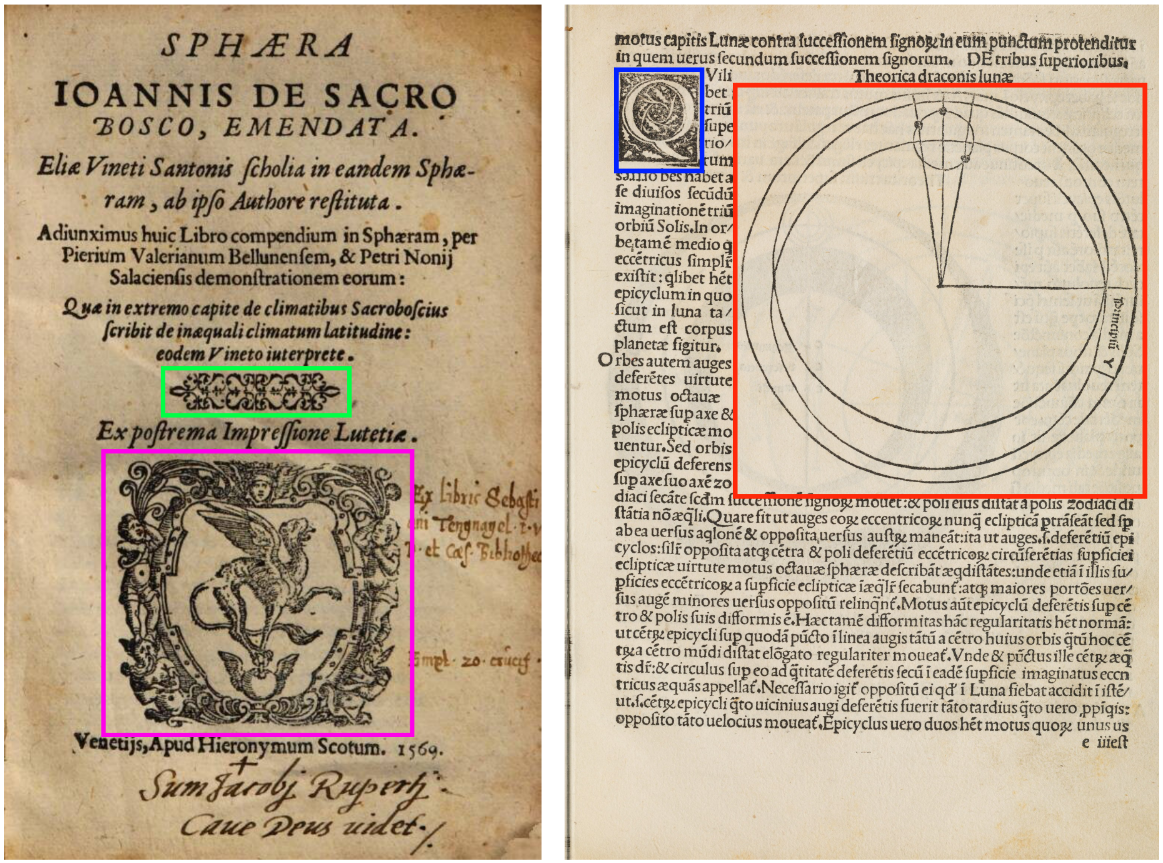
\includegraphics[scale=0.3]{img/s-ved.png}
	\caption{Deux pages du dataset S-VED (2022) représentant les quatre classes du vocabulaire de description du document.}
	\label{fig:s-ved}
\end{figure}

Pour notre tâche de constitution de corpus, nous avons donc dû réaligner de nombreux jeux de données présentant ce genre de défauts dans leurs vocabulaires contrôlés, qu'il s'agisse de descriptions de manuscrits ou d'imprimés. De plus, nous étions soumis à des contraintes de temps (l'ontologie ne devait pas être trop complexe) et de ressources humaines (un travail confié à un profil généraliste confronté à une grande diversité de typologies documentaires). Nous avons donc obéi à une règle en trois points : les classes au sein de notre ontologie doivent être uniquement visuelles (asémantiques), applicables à plusieurs typologies de documents comme les manuscrits et les imprimés (généralistes), et elles ne doivent pas pouvoir se confondre (absence de chevauchements ou \textit{overlaps}). Nous avons nommé cette règle \gls{agc}.

\begin{table}
\centering
\ra{1.25}
\caption{Comparaison des ontologies utilisées selon notre principe \gls{agc} dans l'annotation de différents jeux de données}
\label{tab:datasets-comparison}
	\begin{tabular}{lcccc}
	\toprule
	\textbf{Nom} & \textbf{Asemantic} & \textbf{Generalistic} & \textbf{Classes overlaps} & \textbf{Format} \\
	\midrule
	IlluHisDoc & {\color{red}\faClose} & {\color{green}\faCheck} & {\color{red}\faClose} & Per pixel  \\
	S-VED & {\color{red}\faClose} & {\color{green}\faCheck} & {\color{red}\faClose} & Per pixel  \\
	Horae-LSv2 & {\color{red}\faClose} & {\color{red}\faClose} & {\color{red}\faClose} & Yolo  \\
	SegmOnto & {\color{green}\faCheck} & {\color{green}\faCheck} & {\color{red}\faClose} & other XML \\
	Newspaper Datasets & {\color{red}\faClose} & {\color{red}\faClose} & {\color{red}\faClose} & \dots \\
	PrimA & {\color{green}\faCheck} & {\color{red}\faClose} & {\color{red}\faClose} & other XML \\
	DIVAHisDB & {\color{green}\faCheck} & {\color{red}\faClose} & {\color{red}\faClose} & PAGE XML \\
	DMAS2019 & {\color{red}\faClose} & {\color{red}\faClose} & {\color{red}\faClose} & PAGE XML \\
	\textbf{GenHisDoc} & {\color{green}\faCheck} & {\color{green}\faCheck} & {\color{green}\faCheck} & Yolo \\
\bottomrule
\end{tabular}
\end{table}

\subsubsection{La réalité humaine de la tâche d'annotation}

Durant la création d'une ontologie, le chercheur ou la chercheuse va tendre vers une forme d'exhaustivité descriptive pour rendre compte de la complexité de ses sources. Or, la vision par ordinateur fait face à des contraintes statistiques strictes qui entrent en contradiction directe avec ce besoin de précision historiographique. 

Cette volonté d'exhaustivité se heurte à ce que l'on nomme \textit{long-tail distribution}\footnote{Chongsheng Zhang, George Almpanidis, Gaojuan Fan, Binquan Deng, Yanbo Zhang, \og A Systematic Review on Long-Tailed Learning \fg, publié sur ArXiv, DOI : \href{https://doi.org/10.48550/arXiv.2408.00483}{https:\/\/doi.org/10.48550\/arXiv.2408.00483}} des classes au sein des annotations du dataset. Concevoir une ontologie dotée de dizaines de catégories très spécifiques (les annotations de lettrines au sein de Horae, par exemple) crée un déséquilibre statistique. Le modèle manquera d'exemples d'entraînement pour les classes les plus rares, ce qui se traduira par un taux de rappel quasi nul pour ces dernières. De plus, cette grande variété dans les choix d'annotation démultiplie la complexité de la tâche d'annotation humaine. Ce travail, exigeant et répétitif, repose très souvent sur des opérateurs humains (étudiants, stagiaires, vacataires) soumis à une forte charge cognitive. Plus le nombre de classes augmente, plus l'ambiguïté grandit face à un document historique souvent dégradé, ce qui fait inévitablement chuter l'accord inter-annotateurs (\gls{iaa}) et produit ainsi un jeu de données bruité. 

Pour pallier ce problème tout en préservant les fonctionnalités nécessaires à la recherche, Il existe deux solutions : 

Pour AIKON, au vu des moyens et du temps disponible, nous avons décidé d'utiliser une ontologie minimale avec des classes très englobantes. Par exemple, \textit{Illustration} englobe toutes les illustrations d'un livre d'heures, mais également les schémas mathématiques d'un manuscrit ou les photographies d'une page de journal. Cela diminue forcément la précision d'un modèle, mais c'est le choix que nous avons fait pour GenHisDoc. 

Une autre solution réside dans la construction d'une ontologie hiérarchique\footnote{Ghassan Beydoun, Antonio A. Lopez-Lorca, Francisco García-Sánchez, Rodrigo Martínez-Béjar, \og How do we measure and improve the quality of a hierarchical ontology? \fg, dans \textit{Journal of Systems and Software}, n°84, vol 12, pp. 2363-2373, 2011}. Il s'agit d'un vocabulaire contrôlé qui utilise des relations de subsomption (le principe du \textit{is-a} ou \og est un \fg). Cette structuration en arbre permet de regrouper les classes rares sous des macro-catégories plus larges. D'un point de vue informatique, cela autorise l'entraînement du modèle avec une fonction de perte hiérarchique (\textit{hierarchical loss}). Ainsi, si le réseau de neurones, ou l'annotateur humain en amont, hésite sur la sous-classe exacte d'un objet en raison d'une ambiguïté visuelle, il peut au moins assigner ou prédire correctement la classe supérieure (par exemple, identifier formellement une \textit{Lettrine} plutôt que de se tromper entre une lettrine historiée et une lettrine enluminée). L'erreur est alors atténuée et l'accord inter-annotateur beaucoup plus fort, le modèle n'est donc pas brutalement pénalisé pour une classification imparfaite au niveau de la sous-classe, et la tâche de l'annotateur est potentiellement allégée.

% parler du fait que corriger est en fait plus long qu'annoté une page vierge

\subsection{Vers une \og nouvelle économie de l'érudition \fg{} : la vision et les pratiques des chercheurs}

La création d'une vérité de terrain en vision par ordinateur est, nous l'avons vu, une tâche chronophage et coûteuse, tant dans la modélisation conceptuelle (l'ontologie) du document que dans la production effective des annotations. Pour répondre à ces contraintes de temps et de moyens, le champ de la vision artificielle appliquée aux documents historiques s'oriente vers le développement de projets et de plateformes de partage de jeux de données, conçus pour favoriser leur réutilisation et leur interopérabilité.

\subsubsection{Du « goût de l'archive » à une recherche collective : les enjeux méthodologiques de l'intermédiation numérique}

L'histoire est une discipline profondément auto-réflexive, traditionnellement attachée au contact direct, physique et sensuel avec la source. Ce que l'historienne Arlette Farge a nommé le \og goût de l'archive \fg\footnote{Arlette Farge, \textit{Le Goût de l'archive}, éditions du Seuil, 1989.} repose sur une relation intime entre le chercheur individuel et le document matériel. Or, l'introduction de la vision artificielle dans le travail de dépouillement modifie cette relation en imposant une intermédiation technologique qui peut sembler opaque. 

Les historiens se sont saisis de l'outil informatique avec deux utilisations principales : l'édition de sources et la mise en base de données qui permettent de partager des résultats. Dans le domaine de la vision, il existe déjà des outils et des modèles capables de produire des résultats utiles, mais la barrière d'entrée lié à la complexité de réutilisation des données et des moyens à investir pour pouvoir produire de nouvelles données sont trop élevée pour la plupart des chercheurs menant des travaux individuels ou pour la plupart des laboratoires universitaires en général. Quand on veut y intégrer des méthodes de \textit{machine learning}, la recherche ne peut plus s'envisager comme une démarche purement solitaire. Elle devient dépendante d'infrastructures techniques complexes (serveurs de calcul) et d'un travail collectif en amont (ingénieurs, annotateurs, hébergement).

En France, l'initiative la plus proche d'une telle infrastructure est le projet Gallicorpora. Conçu pour la constitution de jeux de données d'entraînement et le développement d'outils de conversion des standards de la \gls{bnf} vers la \gls{tei}, cet écosystème fournit des corpus d'images finement annotées combinant transcription textuelle et segmentation de la mise en page pour des imprimés allant du XVe au XIXe siècle. Un autre exemple sont les jeux de données de l'équipe \gls{almanach} de l'\gls{inria} avec les jeux de données CATmus\footnote{Thibault Clérice, Ariane Pinche, Malamatenia Vlachou-Efstathiou, Alix Chagué, Jean-Baptiste Camps, et al.. \og CATMuS Medieval: A multilingual large-scale cross-century dataset in Latin script for handwritten text recognition and beyond. \fg communication pour \textit{2024 International Conference on Document Analysis and Recognition (ICDAR)}, pp.174-194, 2024} puis CoMMA\footnote{Thibault Clérice, Simon Gabay, Malamatenia Vlachou-Efstathiou, Ariane Pinche, Benoît Sagot. \og CoMMA, a Large-scale Corpus of Multilingual Medieval Archives \fg, publié sur HAL, 2025,  Hal ID : hal-05299220v1⟩}. Toutefois, pour les autres tâches de vision par ordinateur, comme l'analyse de mise en page avancée, la segmentation ou la détection d'éléments visuels, il n'existe toujours pas d'initiative fédératrice assurant la mutualisation des données produites. De plus, à l'exception notable de la démarche SegmOnto, la communauté manque encore de benchmarks permettant d'évaluer l'efficacité des ontologies et d'attester que les données générées répondent à un véritable intérêt scientifique.

Dès lors, comment définir ce qui constitue une \og bonne \fg{} ontologie pour l'étude des documents historiques, et sur quels critères la privilégier face à une autre ? Comme nous l'avons vu, son évaluation ne saurait se limiter aux seules métriques de performances algorithmique. Pour un usage historique, une ontologie pertinente se juge donc en deux temps : opératoire et heuristique.

D'un côté, elle doit assurer une robustesse statistique en limitant l'ambiguïté pour les annotateurs humains et la machine, un défi auquel tentent de répondre des principes de conception que nous avons évoqué plus tôt. De l'autre, sa valeur réelle se mesure à son intêret scientifique. Face à deux vocabulaires contrôlés concurrents, l'ontologie supérieure est celle qui garantit la meilleure interopérabilité des données produites, permettant ainsi le croisement de corpus matériels hétérogènes.

Pour le choix entre deux vocabulaires contrôlés concurrent, l'ontologie supérieure est en réalité celle qui garantit la meilleure interopérabilité des données produites. Nous laissons donc derrière nous une partie des jeux de données ayant des systèmes d'annotations exhaustives souvent confinés à des projets uniques, au profit de grilles de lecture articulées autour du principe de généralisation. 

\subsubsection{Le standard \gls{iiif} et ses atouts pour l'Open Data}

En informatique, la validité d'une démarche repose sur la reproductibilité des résultats, et donc la possibilité de réexécuter un traitement sur un même jeu de données. En histoire, la scientificité d'une démonstration s'appuie sur la critique des sources et la possibilité, pour les pairs, de vérifier l'appareil critique. La rencontre entre ces deux exigences démontre que la scientificité de l'utilisation de méthodes de machine learning pour l'analyse de documents passe par l'ouverture des données d'entrainement.

Dans ce contexte, l'adoption de standards techniques partagés devient incontournable, au premier rang desquels figure le protocole \gls{iiif}. Ce cadre a profondément transformé l'accès aux corpus patrimoniaux en permettant de manipuler, de comparer et d'annoter des images à très haute résolution provenant de différentes institutions (\gls{bnf}, bibliothèques universitaires, musées) sans forcément avoir à télécharger, ni à dupliquer ces lourds fichiers. Plus encore, grâce aux standards du Web sémantique (comme le \textit{Web Annotation Data Model}), les prédictions générées par la vision artificielle (boîtes englobantes, polygones de segmentation) peuvent être partagées sous forme de surcouches textuelles légères (fichiers JSON) pointant directement vers les \gls{uri} des images distantes. L'utilisation de \gls{iiif} au sein d'application de vision permet un meilleur usage et partage des données des institutions patrimoniales et des données de la recherche qui en découlent. 

L'intégration native de \gls{iiif} au sein du projet AIKON s'inscrit pleinement dans cette dynamique. En proposant un environnement utilisateur capable de se brancher directement sur les entrepôts numériques des institutions patrimoniales, l'application facilite la constitution de corpus personnalisés et le déploiement de modèles de détection sans friction technique. Ce choix architectural contribue à une meilleure diffusion des données de la recherche : les chercheurs peuvent importer leurs sources, exécuter une tâche de détection, puis exporter et partager leurs résultats sous des formats ouverts. Cet écosystème interopérable est ainsi pensé pour s'insérer naturellement dans le cycle de vie de la donnée patrimoniale et encourager un partage continu des connaissances au sein de la communauté scientifique.
\chapter[Le projet Aikon]{Le projet Aikon}

\section{Le contexte et les objectifs du projet Aikon}

\lettrine{A}{ikon est} une plateforme modulaire et open-source de vision par ordinateur, spécifiquement conçue pour les historiennes, les historiens et les chercheurs en humanités numériques. Son objectif principal est de mettre des algorithmes d'intelligence artificielle à la disposition d'utilisateurs ne possédant pas d'expertise technique en informatique. 


\subsection{Les objectifs scientifiques de la plateforme}
Les problématiques directement au coeur de la plateforme et de son utilisation sont : 

\begin{description}
\item[Comment mettre à disposition ces modèles aux chercheurs en SHS ?] Aikon n'est pas un projet de recherche lié à un sujet historique en particulier, c'est au contraire un projet fédérateur autour d'enjeux d'apport de la technique dans la méthode et donc un travail autant lié aux questions d'applicabilité des technologies d'intelligence artificielle que de l'évolution de l'historiographie au contacte des nouvelles méthodes informatiques. 

L'objectif de service de la plateforme est de permettre aux chercheurs de pratiquer une lecture distante\footnote{T. Arnold and L. Tilton, \og Distant Viewing: Analyzing Large Visual Corpora.\fg dans \textit{Digital Scholarship in the Humanities}, 2019} (\textit{distant viewing}) sur des corpus visuels massifs. Cette démarche s'appuie sur le traitement en masse pour transformer des documents en données exploitables. Aikon propose de récupéré de manière automatique des éléments structurants des documents comme les illustrations et d'y rechercher des régularités, des similarités. les visualisations globales (graphes, cartographies, représentations de similarité) permettent de faire émerger des tendances suspectées à l'œil humain à l'échelle d'un corpus entier, afin d'orienter le chercheur vers des cas d'études précis à analyser en détail.

\item[Comment obtenir des annotations expertes en pour affiner leurs prédictions ?] AIKON développe un paradigme interactif de \og l'humain dans la boucle \fg   (\textit{Human-in-the-loop}). L'approche \textit{HITL} offre une réduction de la pénibilité du travail d'annotation car la correction d'erreurs pré-existantes est nettement plus rapide et moins épuisante que le détourage manuel de milliers d'éléments visuels tout en résolvant le problème du manque de données de qualité annotées. De plus cette approche garantit à l'équipe d'Aikon et équipes de chercheurs un contrôle total sur les données qui servent à entraîner les outils d'analyse. La plateforme est développée selon les besoins des utilisateurs et attire des publics travaillant sur des sources très différentes. Le fait d'avoir autant de spécialistes de documents rares et difficiles, versant leurs fonds sur Aikon pour les étudier ouvre la voie à la constitution de datasets historiques précieux. L'un des objectifs scientifique d'Aikon et l'un des objectifs de notre stage est de réadapté des données d'annotation de documents en corpus d'entraînement pour de nouveaux modèles plus performants.
\end{description}

\begin{figure}[h]
    \centering
    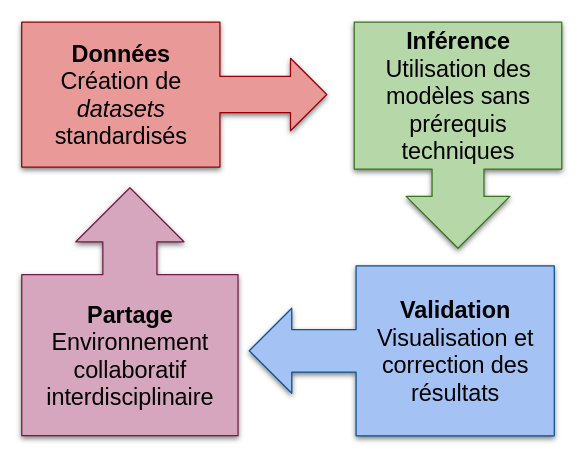
\includegraphics[scale=0.5]{img/aikonmethod.png}
    \caption{Le paradigme \textit{Human in the Loop} dans le projet Aikon}
    \label{fig:HITL}
\end{figure}

\subsection{Les réalisations techniques du projet}

Pour réussir ses missions, le méthodologie de l'équipe d'Aikon est de mettre en place un environnement perdurant sur long terme, étant capable de produire ses propres données d'entraînement avec l'aide de sa communauté de recherche et d'utilisateurs. 

Voici actuellement les fonctionnalités présentes sur les différentes instances de l'application d'Aikon\footnote{Informations tirées de la \href{https://docs.google.com/presentation/d/e/2PACX-1vTZ1cwAzy9YppXFgB3q9P-BXkFGck8F0FzdvrlTMDxhRdHxaPhinTWAIKyT_GATYEAgWEEE1mXrQvDt/pub?start=false&loop=false&delayms=3000\#slide=id.g306b6d3dc05_0_273}{présentation Aikon}} : 

\begin{description}
    \item \textbf{Documenter des sources historiques :} 
    Aikon offre une interface et un modèle de données conçu pour l'étude du lien intellectuel entre les sources. 
    
    \item \textbf{Gérer les numérisations des chercheurs:}
    Ensuite, les chercheurs peuvent importer leurs propres bases de données (images JPEG, PDF, IIIF \dots). La plateforme s'appuie sur le standard de référence IIIF (\textit{International Image Interoperability Framework}) pour gérer les images et les annotations, garantissant une forte interopérabilité avec les systèmes des bibliothèques et des archives. En s'appuyant sur les manifestes pour la gestion des images et des annotations, la plateforme s'insère de manière fluide dans n'importe quelle chaîne de traitement patrimoniale respectant ce standard comme par exemple \textit{Aikoncli}, un CLI développé durant le stage pour récupérer les annotations au format Yolo à partir d'un manifeste IIIF Aikon.  
    
    \item \textbf{Créer des corpus cohérents pour des traitements groupés :}
    Aikon offre une interface de gestion de la page à l'échelle du corpus de documents. 
    
    \item \textbf{Le traitement automatique des sources :} L'interface permet d'exécuter des tâches d'inférence sur les documents pour des analyses variées, comme l'extraction d'illustrations, de filigranes, la recherche de similarités visuelles entre plusieurs images, le regroupement (clustering) ou encore la vectorisation des diagrammes mathématiques.

    \item \textbf{La validation et la correction des résultats :} La plateforme est pensée pour l'interaction humaine. Les chercheurs peuvent annoter les documents et corriger les prédictions des modèles. Cela permet non seulement d'affiner leurs recherches, mais aussi de produire des données d'entraînement de qualité (vérité de terrain) qui pourront être réutilisées par les informaticiens pour améliorer les algorithmes.
\end{description}

Le projet est en cours de développement et d'amélioration actif avec notamment la détection des lignes et des régions d'écritures, du traitement des écritures (OCR/HTR), de la détection multiclasse\dots

\section{Les projets de recherche en vision artificielle historique}

Actuellement, la majorité des projets utilisant Aikon sont des consortiums de recherche en histoire des sciences. 

\subsection{Le projet Aikon et ses collaborateurs}


\begin{description}

\item[IMAGINE :] Imagine est un groupe de recherche hébergé à l'École Nationale des Ponts et Chaussées (ENPC, rattachée à l'Institut Polytechnique de Paris). Situé près de Paris, il fait partie de l'équipe A3SI au sein du laboratoire d'informatique Gaspard-Monge (LIGM). Les domaines de recherche d'Imagine sont la vision artificielle et l'apprentissage automatique\footnote{Site institutionnel d'\href{https://imagine-lab.enpc.fr/}{Imagine}}.

\begin{description}
    \item \textbf{ERC DISCOVER :} Porté par Mathieu Aubry au sein du laboratoire LIGM, Discover\footnote{Site institutionnel de \href{https://erc-discover.github.io/}{Discover}} est un projet de recherche fondamental financé par le Conseil Européen de la Recherche (bourse ERC Consolidator Grant). Le but est de développer la recherche en vision artificielle sur les \textit{structures visuelles} dans les domaines de la vision artificielle appliquées aux documents historiques et dans le domaine de l'imagerie terrestre. 
    
    Le projet Aikon est financé par Discover sous l'impulsion de Mathieu Aubry et Ségolène Albouy. L'objectif est de prouver que l'état de l'art de la vision artificielle peut être directement manipulé par des historiennes et des historiens sans prérequis en programmation informatique. L'une des grandes spécialités de l'équipe réside dans l'analyse de la similarité visuelle et la correspondance de motifs complexes. Dans l'application Aikon, cette expertise se traduit par des fonctionnalités de clustering et de recherche d'images par le contenu. Les informaticien\pmm nes d'IMAGINE travaillent également à de meilleurs algorithmes d'OCR et d'HTR à intégrer dans Aikon. 
\end{description}

\item[EIDA :]

\textit{Editing and Analysing hIstorical astronomical Diagrams with Artificial intelligence} est un projet coordoné par l'historien Matthieu Husson, lié à l'Observatoire de Paris et financé par l'Agence nationale de la recherche. C'est un programme d'étude d'histoire de l'astronomie à l'aide de technologies de vision artificielle en lien avec les autres activités de Matthieu Husson d'analyse des sources anciennes (notamment à travers la conception du système d'information DISHAS et la direction du projet européen ERC ALFA)

EIDA s'attaque au langage visuel et géométrique de la science. L'objectif est de détecter, d'extraire, de classifier et de comparer automatiquement les diagrammes astronomiques. L'enjeu historique est de comprendre comment le savoir scientifique (modèles cosmologiques, calculs d'éclipses, mouvements planétaires) a circulé, été copié et modifié à travers l'Europe et le bassin méditerranéen.

Le projet se concentre sur les manuscrits médiévaux et les premiers incunables (traités d'astronomie, tables astronomiques, commentaires de la Sphère de Sacrobosco). Ces documents sont particulièrement complexes car le texte s'enroule souvent autour des diagrammes, et les figures géométriques varient énormément selon la main du copiste.

L'une des spécificités du projet est l'étude des tables astronomiques. L'étude des données tabulaires est l'un des sujets qui a été le plus difficile au sein de la création du corpus GenHisDoc dont l'un des objectifs était de réussir à détecter les tables dans les documents historiques. 

\item[Le projet VHS :] \textit{Vision and Historical analysis of Scientific illustration circulation} est coordoné par l'historien des mathématique Alexandre Guilbaud et supporté par Sorbonne Université et l'Agence nationale de Recherche. C'est un projet au croisement de l'histoire de l'art, de l'histoire des sciences et des humanités numériques. Il s'agit d'un programme interdisciplinaire associant plusieurs institutions, notamment Sorbonne Université (via l'Institut des sciences du calcul et des données --- ISCD, et le laboratoire LIP6), le CNRS (Orient \& Méditerranée) et l'équipe IMAGINE de l'École des Ponts ParisTech.

Le but scientifique de VHS est d'appliquer les méthodes d'apprentissage profond (Deep Learning) pour analyser la circulation et la réutilisation des images dans l'histoire scientifique ou culturelle. Il s'agit de repérer des motifs récurrents, de tracer l'évolution d'une iconographie au fil des siècles, et de constituer des stemmata grâce à l'étude a similarité visuelle entre les illustrations. L'ambition centrale du projet VHS est de renouveler l'approche historique de la circulation des savoirs scientifiques en se focalisant non plus sur le texte, mais sur l'image et la pensée visuelle.  

Les corpus sont souvent plus hétérogènes que ceux d'EIDA. Ils englobent des imprimés richement illustrés, des estampes, des planches anatomiques ou botaniques, et des schémas techniques. L'enjeu pour le modèle de vision n'est pas seulement de détecter \og où \fg~est l'image (détection d'objet), mais de comprendre \og de quoi \fg~elle est proche visuellement dans le reste du corpus.


\end{description}

\subsection{Les autres projets de vision artificielle historique :}

Parmi les projets de recherche appliquant la vision artificielle à l'histoire et aux humanités numériques, certains sont dotés de plateformes en ligne qui proposent à l’utilisateur d’explorer leurs corpus visuels et de découvrir leurs travaux. Dans la conception de l’application du projet AIkon et de la capacité des modèles à entrainer, il est essentiel de proposer des fonctionnalités d’analyse et d'exploration visuelle qui viennent compléter les outils existants. Dans cette mesure, l’examen des dispositifs de recherche par l'image et de détection actuels, tout comme l'identification de leurs limites, s'avère éclairant pour cibler les besoins des utilisateurs dans le cadre d’un projet collaboratif, tout en prenant en compte la diversité des approches face aux sources iconographiques.


\begin{description}
    
        \item[Le Consortium Pictoria :] Le \textit{Programme d'Identification, Classification, Traitement d'Images, Observation et Reconnaissance des formes par l'Intelligence Artificielle}\footnote{Site institutionnel de  \href{https://pictoria.hypotheses.org/}{Pictoria}} est un consortium-HN supporté par la Maison des Sciences Humaines et Sociales Mondes et coordonné par Julien Schuh. Cette initiative fédère la recherche interdisciplinaire autour de la reconnaissance automatique de formes appliquée aux sciences humaines et sociales. Son action vise à faciliter l'accès, l'interconnexion et l'enrichissement des corpus visuels (histoire de l'art, archéologie, histoire de l'architecture, sociologie, etc.) en développant des protocoles partagés, des formations, des tutoriels ainsi que des prototypes applicatifs.

        Porté par une dynamique nationale et internationale, le projet réunit des laboratoires de recherche ainsi que des institutions patrimoniales de premier plan, parmi lesquelles la BnF, l’INHA, l’INA, l’École nationale des chartes ou encore La contemporaine ...

        Pictoria met à disposition des notebooks jupyter de tutoriels pour les chercheurs ainsi que des listes d'outils sur SSH Open Market Place et contribue à faire conna\^itre le projet Aikon. 
        
        \item[Gallica :] 
        
        La BnF propose ou a proposé plusieurs projets liés à la vision artificielle historique notamment par le travail de Jean-Philippe Moreux. 
        
        --- La BnF propose par sur son site BnF Api\footnote{Lien vers le \href{https://api.bnf.fr/fr/node/181\#scroll-nav\_\_1}{site institutionnel de l'api BnF}} des collections de jeu de données d'images annotés pour la classification.
        
        --- GallicaPix, un démonstrateur qui n'est plus en ligne aujourd'hui, de recherche visuelle de détection et de segmentation des images (cartes, gravures, photographies) 
        
        Nous avions étudié le fait de réutiliser des jeux de données Gallica, la complexité de réutilisation des formats d'annotations dans un temps très court nous à amener à envisager d'autres jeux de données. 
        
        \item[Arkindex / Teklia :] Développée par une entreprise française cette plateforme couple HTR, classification de page, détection et segmentation. Arkindex est notamment utilisé par le projet SocFace réunissant l'Institut national d'études démographiques (INED), les Archives nationales et Teklia. 
        
        Le dataset Horae de l'IRHT publié sur Zenodo a notamment été produit en utilisant Arkindex et des modèles entraînés sur Horae peuvent y être testé.  Contrairement à l'application Aikon actuelle, Arkindex peut travailler avec du texte imprimé et manuscrit et donc les données qui en sortent sont bien plus complexes qu'un simple dataset de détection. Nous avons donc étudier l'ontologie d'annotation d'Horae directement sur Arkindex avant de télécharger et modifier le dataset pour nos propres besoins.
        
        De la même manière que AIkon, Arkindex permet de déployer plusieurs modèles différents sur la même plateforme pour plusieurs types de tâches et d'utiliser cette méthode d'\textit{Human in the loop} pour pré-annoter et corriger des corpus. 
        
        \item[Newspaper Navigator / Library of Congress, USA :] Issue du projet \textit{Chronicling America}\footnote{Site institutionnel du \href{https://labs.loc.gov/work/experiments/newspaper-navigator/}{projet Newspaper Navigator}} et mené par Benjamin Lee. Ce projet s'appuie sur la détection d'objets pour extraire et indexer des millions de photographies, cartes, dessins et publicités dans les archives de la presse américaine.
        
        Nous sommes allés assez loin dans la réutilisation des annotations de Newspaper Navigator, jusqu'au point que de la correction et de l'incorporation du dataset. Newspaper Navigator était notamment intéressant pour la quantité de photographies et dessins contemporains à l'intérieur, le transfert d'une ontologie d'annotation à une autre était difficile. Nous avons donc retiré tout le corpus de presse avant la phase d'entraînement et d'évaluation des modèles de test.
        
        \item[Machines Reading Maps / Alan Turing Institute :] Un outil d'analyse visuelle\footnote{Site institutionnel du projet \href{https://www.turing.ac.uk/research/research-projects/machines-reading-maps}{Machines Reading Maps}.} permettant aux chercheurs de fouiller des cartes historiques à grande échelle pour y détecter automatiquement des bâtiments, des voies ferrées ou des particularités topographiques.
        
        La question de détecter les cartes au sein du dataset GenHisDoc a été une idée rapidement abandonnée car nous avons considéré qu'une carte au sein d'un texte serait plus simplement détectée comme une illustration et sans réel besoin d'annotation sur mesure. 
        
        \item [dhSegment / Digital Humanities Laboratory :] Développé originalement par Benoit Seguin et Sofia Ares Oliveira. dhSegment est une architecture de deep learning spécifiquement développée pour la segmentation des documents historiques complexes, allant de l'extraction de lignes à la détection de bordures et d'illustrations.
        
        Nous nous sommes rapidement orienté vers une approche de détection d'éléments plutôt que de segmentation. Cependant la dhSegment a été l'une des sources envisagée pour la création de masques de segmentation ou la conversion masque de segmentation vers boîtes englobantes. 

        \item[TORNE-H / École nationale des chartes \& Musée des arts décoratifs :] Coordoné par Mme Emmanuelle Bermès, le projet Torne-H développe des outils et des méthodes d'utilisation du machine learning dans le monde muséal et archivistique. L'application TiamaT (\textit{Toolkit for Integrated Annotation and Machine-learning Assisted Training}), développée par Marion Charpier et Fantin Le Ber s'attaque comme Aikon à la question de la préannotation des données pour l'entrainement de modèles avec le m\^eme paradigme d'amélioration itérative \textit{Human in the Loop}\footnote{Présentation de TiamaT sur \href{https://marketplace.sshopencloud.eu/tool-or-service/lYN2OC}{SSHopen Marketplace}}.
        
\end{description}

\part{Construire un corpus de numérisations pour le traitement par  vision artificielle}

\section*{Introduction}
\sectionmark{Introduction}

\begin{quote}
    \textit{Depuis au moins cinquante ans, les historiens adoptent continuellement des méthodes issues des sciences naturelles, des sciences mathématiques et des sciences des données, intégrant ainsi des facteurs non humains à leur champ d'interprétation
grâce à de nouveaux outils (facteurs climatiques, épidémiologiques, datation par des méthodes physiques, etc.). Cependant, le traitement des sources historiques par l'IA pose des défis particuliers aux historiens, même dans ce contexte.
}

Alexandre Guilbaud, Matthieu Husson, Stavros Lazaris, Ségolène Albouy, Somkeo Norindr, Paul
Kervegan, Fouad Aouinti, Robin Champenois, Rémy Delanaux, Mathieu Aubry, \og AIKON: A Collaborative Research Environment for the Visual Study of Historical Corpora \fg, publié sur HAL, HAL ID : \href{⟨hal-05249619⟩}{⟨hal-05249619⟩}
\end{quote}

\lettrine{S}{i l'intelligence artificielle } et sa petite soeur,  la vision artificielle, existent depuis longtemps, l'explosion des performances et des moyens attribués à la recherche en IA au tournant des années 2020 rendent ses outils pertinent pour aider l'historien dans ses méthodologies de dépouillement des sources. Nous retrouvons cette tendance au coeur des Humanités Numériques de pouvoir transformer en données analysable au prisme des méthodes informatiques des documents et des sources qui ont historiquement et encore aujourd'hui un travail minutieux et artisanale. 

Cette partie a pour objectif de revenir sur le contexte institutionnel du projet Aikon, projet de mise à disposition d'outils de vision aux historiens par une équipe du laboratoire IMAGINE sous la direction de Mathieu Aubry. Ce projet a pour objectifs d'offrir un environnement de teste aux historiens pour travailler sur leurs sources avec des méthodes informatiques et spécifiquement de vision.

Le cahier des charges du stage était constituer de ces tâches.
\begin{description}
    \item[Intégrer un modèle de détection multiclasse :] Aikon était jusqu'à la construit sur des modèles ne détectant qu'un seul type de région : Illustrations ou diagrammes selon les modèles, une partie de notre mission était également de constituer les premiers essais de détection multiclasse pour Aikon. 
    \item[Évaluer la possibilité de produire un modèle généraliste.] Contrairement aux approches sur-mesure développées pour des corpus très circonscrits, l'enjeu était de concevoir un système de vision  capable de traiter une grande diversité de documents patrimoniaux. Il s'agissait de vérifier si un modèle unique pouvait maintenir de hautes performances prédictives malgré la forte hétérogénéité des époques, des supports matériels (manuscrits, incunables, imprimés modernes) et des mises en page et de trouver les limites d'une approche généraliste.
    \item[Évaluer la possibilité de réutiliser des jeux de données existants.] Cette tâche vise à démontrer la faisabilité technique et épistémologique d'une écologie de la donnée. Il s'agissait d'identifier, de nettoyer et d'harmoniser des corpus ouverts créés par d'autres projets, en résolvant les incompatibilités de formats (conversion de segmentations par pixels en boîtes englobantes) et en alignant leurs ontologies respectives sur la notre.
    \item[Réintégrer des données produites par la communauté d'Aikon.] L'objectif était de valoriser l'expertise documentaire des chercheurs utilisant Aikon. Le stage devait consolider une boucle d'amélioration continue (Human-in-the-loop) permettant d'extraire les annotations et les corrections validées manuellement sur l'interface d'Aikon, afin de les standardiser et de s'en servir comme vérité de terrain pour réentraîner les futurs modèles.
    
\end{description}	
\chapter[Préparer une campagne d’annotation]{Préparer une campagne d’annotation experte : la méthodologie de la fabrique des métadonnées}

\lettrine{L}{'une des} missions de ce stage a été d'entraîner un modèle généraliste. Par \og généraliste \fg, nous entendons un modèle capable d'extraire des éléments visuels indifféremment au sein de documents manuscrits ou imprimés. Ce défi implique de surmonter la forte hétérogénéité visuelle de ces supports, allant de la mise en page normée des débuts de l'imprimerie aux structures plus fluides et parfois altérées des manuscrits médiévaux. L'objectif est d'aboutir à une ontologie suffisamment unifiée et opérationnelle pour s'affranchir du bruit visuel comme des spécificités propres à une époque donnée.

\section[L'ontologie en machine learning]{Qu'est-ce qu'une ontologie en machine learning ?}

\subsection{L'importance de l'ontologie pour les méthodes d'apprentissage automatique}

En vision artificielle, une ontologie d'annotation désigne le cadre conceptuel et structuré qui définit la manière dont les données brutes (ici, des images de documents historiques) doivent être catégorisées et étiquetées pour entraîner un modèle d'apprentissage automatique. Loin de se réduire à une simple liste de mots-clés appliqués sur des boîtes englobantes, il s'agit d'un objet complexe qui s'articule autour de trois dimensions fondamentales :

\begin{itemize}
	\item \textbf{Le vocabulaire (ou taxonomie) :} l'ensemble fini et contrôlé des classes retenues. Dans notre cadre, il réunit les classes \textit{Illustration}, \textit{Lettrine}, \textit{Tampon}, \textit{Ornementation} et \textit{Table}.
	
	\item \textbf{La sémantique :} l'ensemble des règles d'annotation qui définissent la tâche d'annotation, le périmètre d'application du vocabulaire et ses exceptions.
	
	\item \textbf{La structure :} l'organisation des relations entre les classes. Une ontologie peut être hiérarchique (comme le prévoient des standards tels que SegmOnto) ou plate (sans hiérarchie).
\end{itemize}

Le but de la création d'une ontologie est de traduire la complexité et la réalité d'un document historique en un langage fini, compréhensible et traitable tant par des annotateurs humains que par un algorithme. Lors de notre stage, l'enjeu autour de la définition de cette ontologie était double : d'une part, elle influençait directement la manière dont notre modèle allait être réintégré et exploité par les équipes d'AIKON sur l'application ; d'autre part, l'ontologie sous-jacente à \textit{GenHisDoc} constituait l'élément conditionnant la réutilisation de certains jeux de données au détriment d'autres, en fonction de leur schéma d'origine et de la forme technique de leurs annotations. De plus, l'emploi d'une ontologie trop complexe, qui nécessiterait une infrastructure technique lourde, réduirait la facilité de réutilisation des données produites.

\subsection{Les ontologies appliquées aux documents historiques}

Comme nous l'avons souligné précédemment, la plateforme AIKON exploite encore des modèles de détection monoclasses. Une part importante de notre travail a donc consisté à tester la mise en place d'un modèle à la fois généraliste, capable de traiter une grande variété de types de documents, et multiclasse. Dès lors, nous n'avons pas hérité d'une ontologie rigidement fixée plus tôt dans le projet.

\subsubsection{Les ontologies PAGE XML et ALTO XML}

En tant que schémas XML, \gls{page} et \gls{alto} embarquent une ontologie structurelle de la page et constituent aujourd'hui les standards d'export privilégiés par les institutions patrimoniales. Ils sont notamment employés dans le cadre des jeux de données de référence comme ceux du laboratoire \textit{PRImA}, utilisés lors des compétitions internationales de reconnaissance de documents telles que l'\gls{icpr} ou \gls{icdar}.

Dans le détail, \gls{page}\footnote{S. Pletschacher, A. Antonacopoulos, \og The PAGE (Page Analysis and Ground-Truth Elements) Format Framework \fg, \textit{20th International Conference on Pattern Recognition (ICPR2010)}, IEEE-CS Press, pp. 257-260, 2010, DOI : \href{https://doi.org/10.1109/ICPR.2010.72}{10.1109/ICPR.2010.72}.} (\textit{Page Analysis and Ground-Truth Elements}) est développé par le \textit{PRImA research lab} de l'université de Salford (Manchester) et repose sur une architecture hiérarchique. Son ontologie distingue d'abord de grandes régions de blocs (\textit{TextRegion}, \textit{ImageRegion}, \textit{MathsRegion}, \textit{SeparatorRegion}), qui peuvent elles-mêmes être subdivisées en lignes de texte, en mots, puis en glyphes individuels. \gls{page} associe à ses classes des coordonnées géométriques complexes pour des tâches de segmentation fine, ainsi que des métadonnées internes (langue, orientation, typographie).

De son côté, \gls{alto} est un standard maintenu à l'origine grâce au financement européen du projet METAe\footnote{B. Stehno, A. Egger, G. Retti, \og METAe --- Automated Encoding of Digitized Texts \fg, \textit{Literary and Linguistic Computing}, vol. 18, n° 1, pp. 77–88, 2003, DOI : \href{https://doi.org/10.1093/llc/18.1.77}{10.1093/llc/18.1.77}.}. Souvent associé au format de métadonnées de conservation \gls{mets}, il constitue le standard privilégié par de grandes institutions patrimoniales internationales telles que la \gls{bnf} (Gallica) ou la \textit{Library of Congress} qui héberge le schéma officiel depuis 2009. Il se concentre sur la description physique et logique de la page, structurant les blocs de texte, les illustrations et les espaces blancs grâce à des coordonnées exprimées sous forme de boîtes englobantes.

Cependant, si la richesse sémantique et structurelle de ces deux standards garantit une description exhaustive des documents historiques, elle présente une limite majeure dans le cadre technique de notre travail. Ces ontologies sont profondément imbriquées et hiérarchiques. Or, pour entraîner des architectures de détection d'objets rapides et efficaces comme les modèles \gls{yolo} intégrés à AIKON, les données d'entrée doivent idéalement reposer sur une ontologie \og plate \fg. Si certains projets d'envergure disposent des ressources nécessaires pour maintenir des structures aussi complexes, nous avons fait le choix de nous en écarter afin de privilégier un modèle d'annotation direct et aisément convertible.


\subsubsection{SegmOnto}

Au début de notre réflexion, nous nous sommes appuyés sur SegmOnto\footnote{S. Gabay, A. Pinche, K. Christensen, J.-B. Camps, \og SegmOnto: A Controlled Vocabulary to Describe and Process Digital Facsimiles \fg, \textit{Journal of Data Mining and Digital Humanities}, 2024, DOI : \href{https://doi.org/10.46298/jdmdh.12689}{10.46298/jdmdh.12689}.}, l'ontologie de référence pour la description des documents historiques. Si nous en avons conservé la philosophie globale, ancrée dans la description morphologique de la page, nous avons dû nous en écarter pour répondre à une double contrainte, à la fois technique et scientifique.

Sur le plan technique, l'architecture des modèles \gls{yolo} nous imposait de renoncer à toute arborescence complexe au profit d'une ontologie strictement « plate ». Par ailleurs, pour garantir la robustesse de l'apprentissage et éviter un éparpillement statistique des détections, nous avons fait le choix de réduire le schéma à un maximum de cinq classes essentielles.

Sur le plan scientifique, les objectifs du projet AIKON exigeaient un degré de granularité qui entrait en contradiction avec certaines agrégations de SegmOnto. C'est notamment le cas de la classe \textit{GraphicZone}, qui fusionne toutes les expressions picturales. Pour répondre aux besoins de dépouillement historique, nous avons dû réintroduire une distinction fonctionnelle en scindant cette catégorie en deux classes distinctes (\textit{Illustration} et \textit{Ornementation}), en nous inspirant de l'ontologie du jeu de données S-VED.

\begin{table}[h]
    \centering
    \ra{1.2}
    \caption{L'ontologie SegmOnto}
    \label{tab:segmonto}
    \begin{tabular}{l l}
        \toprule           
        \textbf{Classes SegmOnto} & \textbf{Définition} \\
        \midrule
        CustomZone & ... \\
        DamageZone & Dégâts sur le document \\
        DigitisationArtefactZone & Dégâts sur l'image numérisée \\
        DropCapitalZone & Lettrine \\
        GraphicZone & Dessins, Illustration, Ornementation \\
        MainZone & Texte principal au niveau de la page \\
        MarginTextZone & Textes marginaux \\
        MusicZone & Partitions \\
        NumberingZone & Pagination \\
        QuireMarksZone & Réclame \\
        RunningTitleZone & Titres courants \\
        SealZone & Sceaux \\
        StampZone & Estampilles \\
        TableZone & Tables de données \\
        TitlePageZone & Page de titre \\
        \bottomrule
    \end{tabular}
\end{table}

\section[Construire une ontologie d'annotation]{Construire une ontologie d'annotation : de la théorie à la pratique}

Une ontologie aussi synthétique que la nôtre (limitée à cinq classes) déplace la complexité du modèle de représentation des données vers la phase d'annotation manuelle. Il est donc devenu indispensable d'établir des consignes d'annotation strictes afin de départager des éléments graphiquement proches mais fonctionnellement distincts au sein des documents historiques.

\subsection{Définir les frontières sémantiques : le défi des cas limites}

La principale difficulté a résidé dans la distinction entre les éléments relevant de la classe \textit{Illustration} et ceux situés à la frontière entre \textit{Illustration} et \textit{Ornementation}. Dans les manuscrits médiévaux comme dans les premiers imprimés, la frontière entre le décoratif et le figuratif est souvent poreuse. Nous avons fait le choix de nous appuyer sur le rapport au texte : une \textit{Illustration} possède une fonction sémantique ou didactique directe (elle illustre explicitement le propos), tandis que l'\textit{Ornementation} (tels que les bandeaux, culs-de-lampe ou frises marginales) remplit une fonction purement esthétique ou de séparation structurelle.

De la même manière, la classe \textit{Initial} a exigé des règles de délimitation claires. Une lettrine historiée (contenant une scène figurative) devait-elle être annotée comme une illustration ou comme une lettrine ? Pour maintenir la cohérence de l'apprentissage du modèle, nous avons décidé de prioriser la fonction typographique : tout caractère alphabétique agrandi marquant le début d'une section est étiqueté \textit{Initial}, indépendamment de sa richesse iconographique. La prise en compte de cette classe a également nécessité l'étude de plusieurs cas hybrides, notamment des lettres isolées ou d'autres signes typographiques comme le pied-de-mouche (¶), susceptibles d'être confondus avec le motif cible.

La définition de la classe \textit{Table} a elle aussi été source de problèmes. Contrairement aux documents contemporains où les données tabulaires sont généralement structurées par des grilles ou des lignes séparatrices explicites, les documents historiques s'appuient fréquemment sur des structures implicites (alignements par des espaces, listes structurées). Il a fallu déterminer à partir de quel degré de structuration spatiale un bloc de texte devient une \textit{Table}. Nous avons pris le parti de caractériser cette classe par la présence évidente d'une relation bidimensionnelle (lignes et colonnes) porteuse de sens, même en l'absence de lignes de séparation tracées. Pour aider le modèle à repérer cette régularité spatiale, la consigne a été donnée d'englober l'intégralité de la structure logique du tableau, incluant ses en-têtes de colonnes lorsqu'ils sont présents. Enfin, nous avons fait le choix d'exclure de cette classe les structures d'organisation globale du document, telles que les tables des matières ou les index.

\begin{table}[h]
    \centering
    \ra{1.2}
    \caption{L'ontologie de GenHisDoc}
    \label{tab:segmonto}
    \begin{tabular}{l l l}
        \toprule           
        \textbf{Label Yolo} & \textbf{Classes GenHisDoc} & \textbf{Définition} \\
        \midrule
        0 & Illustration & Visuel qui se réfère au texte \\
        1 & Initial & Lettrine \\
        2 & Ornament &  Visuel qui ne se réfère pas au texte \\
        3 & Stamp & Estampille de bibliothèque \\ 
        4 & Table & Données tabulaires \\
        \bottomrule
    \end{tabular}
\end{table}

\subsection{Mettre en place l'ontologie : écrire un guide d'annotation}

Comme le montre l'organigramme~\ref{fig:GenHisDoc}, la rédaction du guide d'annotation a été réalisée \textit{a posteriori} du travail d'annotation et de correction initial. GenHisDoc n'étant conçu que comme un test préalable à une campagne d'annotation de plus grande envergure, la construction de l'ontologie a suivi un processus empirique et itératif : nous avons d'abord annoté un premier volume de données sur divers types de documents, puis arrêté des choix clairs quant à la structure de l'ontologie, avant de procéder à une phase de rétro-correction afin d'harmoniser les données antérieures avant l'entraînement des modèles.

Le but d'un guide d'annotation est de fournir au modèle des données d'apprentissage parfaitement cohérentes grâce à un fort accord inter-annotateurs, tant sur le plan géométrique (précision des délimitations) que sur le respect des règles et exceptions sémantiques propres à chaque classe au sein du document. Dans le cadre d'AIKON, ce guide constitue également un document méthodologique essentiel permettant de conserver une trace explicite des principes retenus, des retours d'expérience et des divers cas limites rencontrés lors de la constitution du jeu de données.

Le guide d'annotation s'articule autour de deux volets principaux. Le premier présente le contexte du projet, définit la tâche d'annotation attribuée et pose les règles générales applicables à l'ensemble des opérations de délimitation.


\subsubsection{Les règles générales}

Les règles générales de cadrage établissent les exigences en matière de rigueur géométrique (c'est-à-dire la méthode précise de tracé de la boîte englobante). Elles imposent notamment un ajustement au plus près des contours de l'objet (\og \textit{hug the border} \fg), la séparation stricte d'éléments visuellement disjoints, ainsi qu'un principe empirique fondamental : l'interdiction d'annoter par déduction ce qui n'est pas directement visible à l'œil humain (\og \textit{annotate what is visible, not what you infer} \fg).

Ces règles générales visent à maximiser l'accord inter-annotateurs et à réduire le bruit lors de l'entraînement des modèles, en évitant d'inclure inutilement de l'arrière-plan ou du texte environnant au sein de la zone délimitée.

\subsubsection{Les règles ontologiques}

D'autre part, la section consacrée aux définitions de classes (\textit{Class definition}) décline, pour chaque étiquette (\textit{Illustration}, \textit{Ornementation}, \textit{Lettrine}, \textit{Tampon}, \textit{Table}), une structure explicite en trois points :

\begin{enumerate}
	\item \textbf{Une description fonctionnelle} rappelant le rôle sémantique et visuel de l'élément au sein de la page ;
	\item \textbf{Des règles d'annotation précises} fixant le périmètre exact de la boîte englobante ;
	\item \textbf{Une analyse des cas limites (\textit{edge cases})} apportant une réponse systématique aux typologies complexes identifiées lors de la phase de test (telles que les lettrines historiées, les encadrements ornés ou les éléments fragmentés).
\end{enumerate}

Outre la rigueur des définitions textuelles, l'usage systématique de figures et la juxtaposition d'exemples concrets (cas validés versus erreurs à éviter) lèvent immédiatement les ambiguïtés. Le format de diffusion de ces consignes s'avère tout aussi déterminant que leur contenu. Pour maintenir un engagement fort et limiter les dérives d'annotation, un guide moderne ne saurait se réduire à un simple document PDF statique : il gagne à être un dispositif dynamique et interactif. Les meilleures directives doivent \og captiver \fg{} l'annotateur dès son intégration grâce à des modules de test ou des quiz d'évaluation, puis s'insérer directement au cœur de l'interface d'annotation afin d'offrir, au simple clic sur une classe, l'affichage instantané de ses cas limites sans jamais quitter l'espace de travail.






\chapter[Construire un corpus historique]{Construire un Corpus historique pour la vision artificielle}

\lettrine{L}{ors de} notre stage, l'objectif à atteindre était de contribuer à la préparation d'une campagne collaborative de constitution d'un jeu de données annoté de documents historiques. L'objectif est de créer un corpus de référence pour l'entraînement de modèles d'extraction automatique de classes visuelles (illustration, photographies, zones de texte, enluminures, etc.). Le stage consistait à définir le cadre méthodologique et technique du dispositif à l'aide de la préparation d'un jeu de données de test.

\section{La nature documentaire du Corpus}

GenHisDoc (\textit{Generalistic Historical Document Dataset}) et ses modèles associés est le jeu de données que nous avons créer lors de ce stage. Les trois questions au coeur de sa création sont : l'harmonisation de corpus hétérogènes pour une réutilisation, l'enrichissement du corpus par la pratique historienne en réutilisant les données produites par Aikon, l'impact que produit une ontologie documentaire sur la performance algorithmique.


\subsection{La réutilisation des jeux de données existants}

Le volume de donnée de qualité pour entraîné un modèle spécialisé performant mieux que ce qui existe déjà demande une autre technique que la création de données \textit{ex nihilo}. De plus, l'un des buts du stage était d'entraîner un modèle aussi efficace sur les livres imprimés que sur les manuscrits. Il existe déjà des corpus spécialisés ouverts et publié sur licence libre permettant une réutilisation et une modification des données. Pour ces raisons de droit, nous avons réutilisé aucune données venant de compétitions comme ICDAR car la plupart sont produit par PRImA Research, un groupe de recherche de l'université de Stalford Manchester dont la plupart des datasets sont sous-droit.

La plupart des jeux de données que nous avons sélectionné pour une réutilisation étaient sous une licence \textit{Creative Common}. Pensez comme un compromis flexible au \og tous droits réservés \fg, les licences\textit{ Creative Commons} offrent un cadre juridique standardisé pour autoriser la libre réutilisation des ressources numériques. En articulant différentes contraintes modulables, de la simple mention de paternité à la restriction des usages commerciaux, ce système simplifie l'ouverture des données patrimoniales et garantit aux chercheurs une sécurité juridique essentielle lors du partage et de la réexploitation des corpus. Dans le domaine de la vision, la plupart des datasets récents utilisent l'attribution 4.0 International (CC BY 4.0) permettant de partager et de réutiliser sur ces ressources à condition de créditer l'auteur original. Dans le cadre de GenHisDoc le crédit ce fait de trois manières : 

\begin{itemize}
    \item Premièrement, dans le README de la publication finale de GenHisDoc, tous les datasets réutilisés sont cités, ainsi que leurs auteurs connus, et les datapapers ayant été publiés pour ces jeux de données.

    \item Deuxièmement, bien que la version du finale du jeu de données mélange ensemble toutes les images et toutes les annotations en deux grands dossiers \textit{Images} et \textit{Annotations}, le script de \og réunification \og des données produit également un lien entre la source de publication de l'image et son nom dans le dataset final disponible dans un format csv. 

    \item Troisièmement, dans le cadre de la réutilisation des données d'Aikon nous nommons les utilisateurs ayant uploadé, inférencé ou corrigé les données que nous avons téléchargé. 

\end{itemize}

Cependant, le potentiel de ces ressources est fréquemment freiné par une hétérogénéité technique et une spécialisation conceptuelle. La première partie de notre travail était d'identifier, agréger et comparer le plus de jeux de données éligible entre eux\footnote{Konstantina Nikolaidou, Mathias Seuret, Hamam Mokayed, Marcus Liwicki, \og A survey of historical document image datasets \fg, dans \textit{International Journal on Document Analysis and Recognition (IJDAR)}, pp.305-338, n°25, vol 4, 2022}. Cette démarche de réutilisation s'est heurtée à deux défis majeurs. Le premier est d'ordre technique avec la diversité des formats d'annotation (segmentation sémantique par pixels, différents types de coordonnés sur l'image pour la boîte englobante) empêche tout entraînement conjoint. Le second étant d'ordre intellectuel où chaque projet de recherche définit son ontologie et ses propres classes d'annotation en fonction de ses problématiques scientifiques, rendant certains jeux de données incompatible entre eux. 

\begin{description}
\item[S-VED :]

\subitem \textbf{Classes :} Illustration, Ornementation, Lettrine, Marque d'imprimeur

\subitem \textbf{Édition :} Issue du projet \textit{De Spherae} de la Max Planck Institute for the History of Science, le dataset S-VED propose un jeu de données constitués d'exemples tirés des 350 éditions du \textit{Tractatus de Spherae} de Johannes de Sacrobosco annotées et compilées ensembles\footnote{Büttner J, Martinetz J, El-Hajj H, Valleriani M, \og CorDeep and the Sacrobosco Dataset: Detection of Visual Elements in Historical Documents \fg, dans \textit{Journal of Imaging}, n°8, volume 10,  pp.285 , 2022,  DOI : \href{10.3390/jimaging8100285}{10.3390/jimaging8100285}}. S-VED  est un projet qui privilégie la simplicité et la facilité d'usage de ses annotations et de son format d'ontologie. S-VED existe en deux versions, une sous-droit et une purgée de ses documents problématiques. Nous avons donc utilisé la deuxième version. Parmi les principales corrections que nous avons du faire à S-VED, la première était la suppression de la classe des marques d'imprimeurs qui ne fait pas sens au sein d'une ontologie généraliste. 

%%%%%%%%%%%%%%%%%%%%%%%%

\item[IlluHisDoc :] 

\subitem \textbf{Classes :} Photographie, Illustration, Dessins, Diagramme scientifiques historiques

\subitem \textbf{Édition :} Issue du projet docExtractor de Tom Monier et Mathieu Aubry\footnote{Tom Monnier, Mathieu Aubry, « docExtractor : An off-the-shelf historical document element extrac-tion »,dans2020 17th International Conference on Frontiers in Handwriting Recognition(ICFHR), pp. 91-96,2020, DOI : 10.1109/ICFHR2020.2020.00027}. D'un point de vue technique, le jeu de données proposait une segmentation sémantique au niveau du pixel, que nous avons transformer en boîtes englobantes au format YOLO\footnote{Jules Musquin avec 4 classes : \href{https://github.com/Anarchiviste/GenHisDoc\_Lab/blob/main/01\_code/reconciliation\_illuhisdoc.py}{scripte reconcialiation\_IlluHisDoc.py sur GenHisDoc\_Lab github}}. D'un point de vue éditorial, la classe très spécifique correspondant aux marques d'imprimeur (printer's marks) a été fusionnée avec notre classe générale \og Illustration \fg afin de maintenir l'approche généraliste de GenHisDoc.

%%%%%%%%%%%%%%%%%%%%%%%

\item[Horae LSv2 :] 

\subitem \textbf{Classes :} Lignes de texte, Lettrines, Ornementations, Zone de texte, Pages, Rubrication, Miniature. 

\subitem \textbf{Édition :} Horae est un jeu de données constitué principalement de livre d'heure. D'un point de vue technique, Horae est déjà pensé pour une compatibilité avec les modèles Yolo. D'un point de vue éditorial, nous avons supprimé toutes les classes liées au texte, regrouper toutes les classes liées aux lettrines, liées toutes les classes liées aux ornementations et liées toutes les classes liées aux illustrations. 

%%%%%%%%%%%%%%%%%%%%%%

\item[El Picpic Stamps :] 

\subitem \textbf{Classes :} Tampons, Signatures
\subitem \textbf{Édition :} C'est à la base un jeu de données publiées sur la plateforme Roboflow sous licence CC by 4.0 par l'utilisateur \textit{El PicPic}. Le jeu de données avait comme but de détecter les tampons et les signatures, nous avons donc supprimés toutes les annotations de signatures. D'un point de vue technique nous avons transformer des boîtes englobantes en coordonnés généraux au format Yolo.

\end{description}

Nous avons aussi travaillé sur l'intégration de documents et de jeux de données qui n'ont pas terminé dans le dataset final. Dans la volonté de produire un jeu de données généraliste capable de fonctionner autant sur un manuscrit médiévale que sur des sources imprimés, nous avons voulu trouver un moyen d'intégrer des sources de presses dans notre ontologie très simple. 

\subsection{Récupérer des données d'Aikon}


Outre l'exploitation de jeux de données publics indépendants, une part déterminante de la constitution de GenHisDoc repose sur la récupération directe de métadonnées produites au sein même de la plateforme AIkon. L'infrastructure d'annotation automatique et de partage des documents dans l'application se fait via le protocole IIIF. Au sein d'Aikon, quand un document récupéré entièrement sur l'application est nommé un \og témoin \fg  (\textit{witnesses}). 

L'utilisation du standard IIIF nous a permis de développer un outil en ligne de commande (CLI) nommé \textit{aikoncli} pour récupérer toutes les pages qui constituent un témoins ainsi que toutes les annotations qui y sont attachées et directement au format YOLO en fournissant le manifeste IIIF de l'instance d'AIkon\footnote{Jules Musquin, \href{https://github.com/Anarchiviste/aikoncli}{\textit{aikoncli} sur GitHub}}.

Les témoins récupérés 
\begin{description}
\item[VHS :] Ce projet interdisciplinaire étudie la circulation de l'illustration scientifique du Moyen Âge à l'ère moderne. Nous avons extrait les données issues de neuf témoins révisés par les chercheurs du projet, couvrant à la fois des imprimés (telle la \textit{Cyclopaedia} d'Ephraïm Chambers) et des manuscrits d'astronomie et de sciences conservés dans de grandes institutions européennes\footnote{Notamment les manuscrits BnF Latin 7416 et Latin 13955 ; ÖNB Cod. 44 et 187 ; Universiteitsbibliotheek Lat. Q. 9 et Voss. Lat. Q. 40 ; Biblioteca Ambrosiana T. 47 ; Sächsische Landesbibliothek Dc 183.}.

\item[EIDA :] Centré sur l'analyse critique des diagrammes astronomiques du VIII\textsuperscript{e} au XVIII\textsuperscript{e} siècle, le projet EIDA apporte une diversité culturelle et typologique indispensable à GenHisDoc. L'extraction a permis d'intégrer des corpus issus de traditions manuscrites non occidentales (sanskrite, turque ottomane, arabo-persane) comme les témoins BnF Sanscrit 964 et Supplément turc 242, ou le manuscrit Sprenger 1838 de la Staatsbibliothek de Berlin.
\end{description}

Une fois un témoin choisi comme étant intéressant à ajouter dans le jeu de données, nous avons fait le choix de ne pas trier les pages internes du document. Le but est de de préserver dans le jeu de données un ratio d'images représentant des pages vides, des pages de titre, des images sans annotations, des images des dos des livres, des images des pages d'information de la BnF insérés dans les pdf téléchargés depuis Gallica. Le but étant de réduire la détection d'élément indésirables en augmentant un peu le bruit dans les données. 

L'intégration de ces corpus d'AIkon représentent un apport précieux pour GenHisDoc, notamment pour la représentativité des schémas et des diagrammes scientifiques. Néanmoins, les modèles historiques d'AIkon fonctionnant sur une détection purement monoclasse (repérant un composant visuel sans qualification typologique), ces données ont donc été traduit par la classe \textit{Illustration} dans l'ontologie de GenHisDoc. 

\section{La nature technique du corpus}

Une fois les sources sélectionnées et l'ontologie décidée, la constitution de GenHisDoc s'est heurtée à la matérialité technique de la donnée brute. Si l'agrégation de corpus issus de projets de recherche indépendants garantit une grande richesse visuelle et historique, elle implique inévitablement une profonde hétérogénéité des choix de formats d'encodage.

Les annotations collectés se présentaient sous des standards divers. Selon les outils utilisés par les chercheurs à l'origine de ces jeux de données, la vérité terrain pouvait prendre la forme de masques de segmentation par pixels (comme pour IlluHisDoc), de coordonnées absolues intégrées dans des fichiers XML, ou encore d'architectures JSON complexes comme pour Aikon. Or, pour fusionner puis corriger et enfin entrainé un modèle nous avons besoin de tout transformer en un seul standard choisi. 

Nous l'avons déjà dit mais Aikon utilise des modèles d'une certains famille. L'enjeu de cette phase de développement a donc consisté à concevoir un pipeline de traitement informatique. Il a fallu d'une part développer des scripts capables d'ingérer ces formats disparates pour les traduire vers le format cible unique exigé par l'architecture YOLO.

\subsection{Faire fonctionner des données entre elles}

La conversion de boîtes englobantes d'un format à l'autre est une question de géométrie, cependant d'autres formats comme les éléments de segmentation au pixel demandent des cha\^ines de traitement beaucoup plus complexe. 

\subsubsection{Travailler avec le format YOLO}


Pour pouvoir entraîner un modèle de la famille des yolo, les prérequis de l'organisation des données sont relativement simple. Les annotations d'image au format yolo font partie d'une des métadonnées les plus simple à mettre en place. Dans un premier temps, le format YOLO impose une structuration simple des fichiers : à chaque document visuel (par exemple \texttt{page\_01.jpg}) doit correspondre un fichier texte d'annotation portant strictement le même nom (\texttt{page\_01.txt}). 

Au sein de ce fichier texte, l'ontologie est traduite de manière spatiale. Chaque ligne correspond à un objet annoté (une boîte englobante) et obéit à une syntaxe standardisée de cinq valeurs numériques séparées par un espace : 
\texttt{<class\_id> <x\_center> <y\_center> <width> <height>}.

\begin{itemize}
    \item \textbf{\texttt{class\_id}} : l'identifiant numérique entier de la classe définie dans l'ontologie (par exemple, 0 pour \textit{Illustration}, 1 pour \textit{Lettrine}, tel que détaillé dans le Tableau \ref{tab:segmonto}).
    \item \textbf{\texttt{x\_center}} et \textbf{\texttt{y\_center}} : les coordonnées du point central de la boîte englobante sur les axes X et Y.
    \item \textbf{\texttt{width}} et \textbf{\texttt{height}} : la largeur et la hauteur totales de la boîte englobante calculé depuis les coordonnées du point central 
\end{itemize}

\begin{figure}[h]
    \centering
    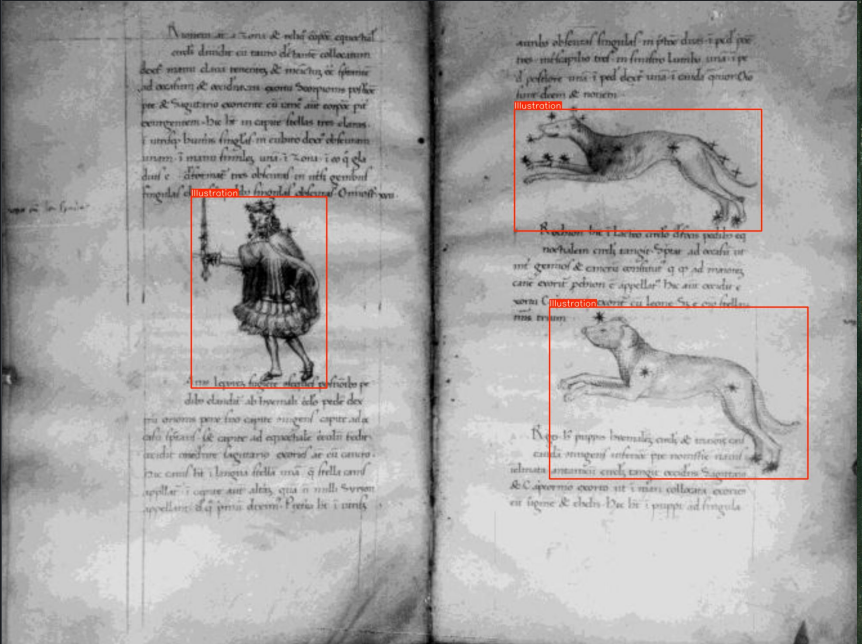
\includegraphics[scale=0.5]{img/aikon.png}
    \caption{Exemple de bounding boxes d'illustrations détectée sur Aikon au format Yolo}
    \label{fig:exemple-aikon}
    
\end{figure}

La particularité de ce format réside dans la normalisation des coordonnées. Les quatre valeurs géométriques ne sont pas exprimées en pixels absolus, mais en proportions relatives (des nombres flottants compris entre 0,0 et 1,0) calculées en fonction des dimensions totales de l'image. Les images d'un jeu de donnée au format yolo peut donc \^etre retravaillées sans avoir à modifier les annotations. 

Par exemple, une ligne d'annotation se présentera sous la forme : \texttt{3 0.18 0.89 0.29 0.18}. 


L'intérêt de ce format comparer à d'autres pour la constitution d'un corpus hétérogène comme GenHisDoc est qu'il permet de s'affranchir de la résolution original, qu'il s'agisse d'une image téléchargé à la résolution maximale d'une api IIIF ou un jeu de données beaucoup plus compressé et donc d'homogénéiser les données d'entrées avant la phase d'apprentissage. 

Certains corpus fournissent déjà une vérité terrain sous forme de boîtes englobantes (\textit{bounding boxes}), mais dans des formats incompatibles avec notre architecture. C'est le cas des formats historiques comme Pascal VOC ou de certains exports XML, qui utilisent des coordonnées absolues basées sur les pixels de l'image.

Généralement, ces formats classiques définissent une zone de deux manières :
\begin{itemize}
    \item Soit par les coordonnées du point supérieur gauche et du point inférieur droit : \texttt{\textbf{x\_min, y\_min, x\_max, y\_max}}
    
    \item Soit par les coordonnées du point supérieur gauche associées à la largeur et la hauteur absolues : \texttt{\textbf{x\_min, y\_min, w\_absolu, h\_absolu}}
\end{itemize}

Puisque le format YOLO exige des coordonnées relatives pointant depuis le centre de l'objet, une étape de conversion mathématique systématique est indispensable. Cette transformation nécessite de connaître les dimensions totales de l'image cible, à savoir sa largeur totale ($W$) et sa hauteur totale ($H$). 

Le passage des coordonnées absolues vers les valeurs normalisées exigées par YOLO s'opère grâce aux calcules suivants :

$$x_{YOLO} = \frac{x_{min} + x_{max}}{2 \times W}$$

$$y_{YOLO} = \frac{y_{min} + y_{max}}{2 \times H}$$

$$w_{YOLO} = \frac{x_{max} - x_{min}}{W}$$

$$h_{YOLO} = \frac{y_{max} - y_{min}}{H}$$

C'est ce calcul par ratio qui garantit au modèle une totale indépendance vis-à-vis de la résolution d'origine des numérisations.


\subsubsection{De la segmentation par pixels aux boîtes englobantes : le cas d'IlluHisDoc}

Plusieurs jeux de données comme IlluHisDoc et SynDoc (non utilisé dans notre travail) fournissaient à l'origine une vértié de terrain sous forme de masque de ségmentation où chaque pixel appartenant à une classe est coloré sur un fond noir. Il a fallu mettre en place un autre pipeline d'extraction géométrique. En utilisant la libraire \textit{Open Computer Vision} en Python, nous avons pu déduire les points extr\^emes des masques\footnote{Jules Musquin, scripte Réconciliation IlluHisDoc sur \href{https://github.com/Anarchiviste/GenHisDoc_Lab/blob/main/01_code/reconciliation_illuhisdoc.py}{Github}} (pixel le plus haut, le plus bas, le plus à gauche et le plus à droite pour chaque forme). À partir de ces limites absolues, nous avons pu retracer les bo\^ites englobantes avec des coordonés abolues et enfin appliqué la méthodologie décrite juste avant pour récupérer des coordonées normalisées au format YOLO. 

\begin{figure}[h]
        \centering
        \begin{subfigure}{0.48\textwidth}
            \centering
            
\includegraphics[scale=0.118]{img/btv1b10532593m_f14_seg.png}
        \end{subfigure}
        \hfill
        \begin{subfigure}{0.48\textwidth}
            \centering
            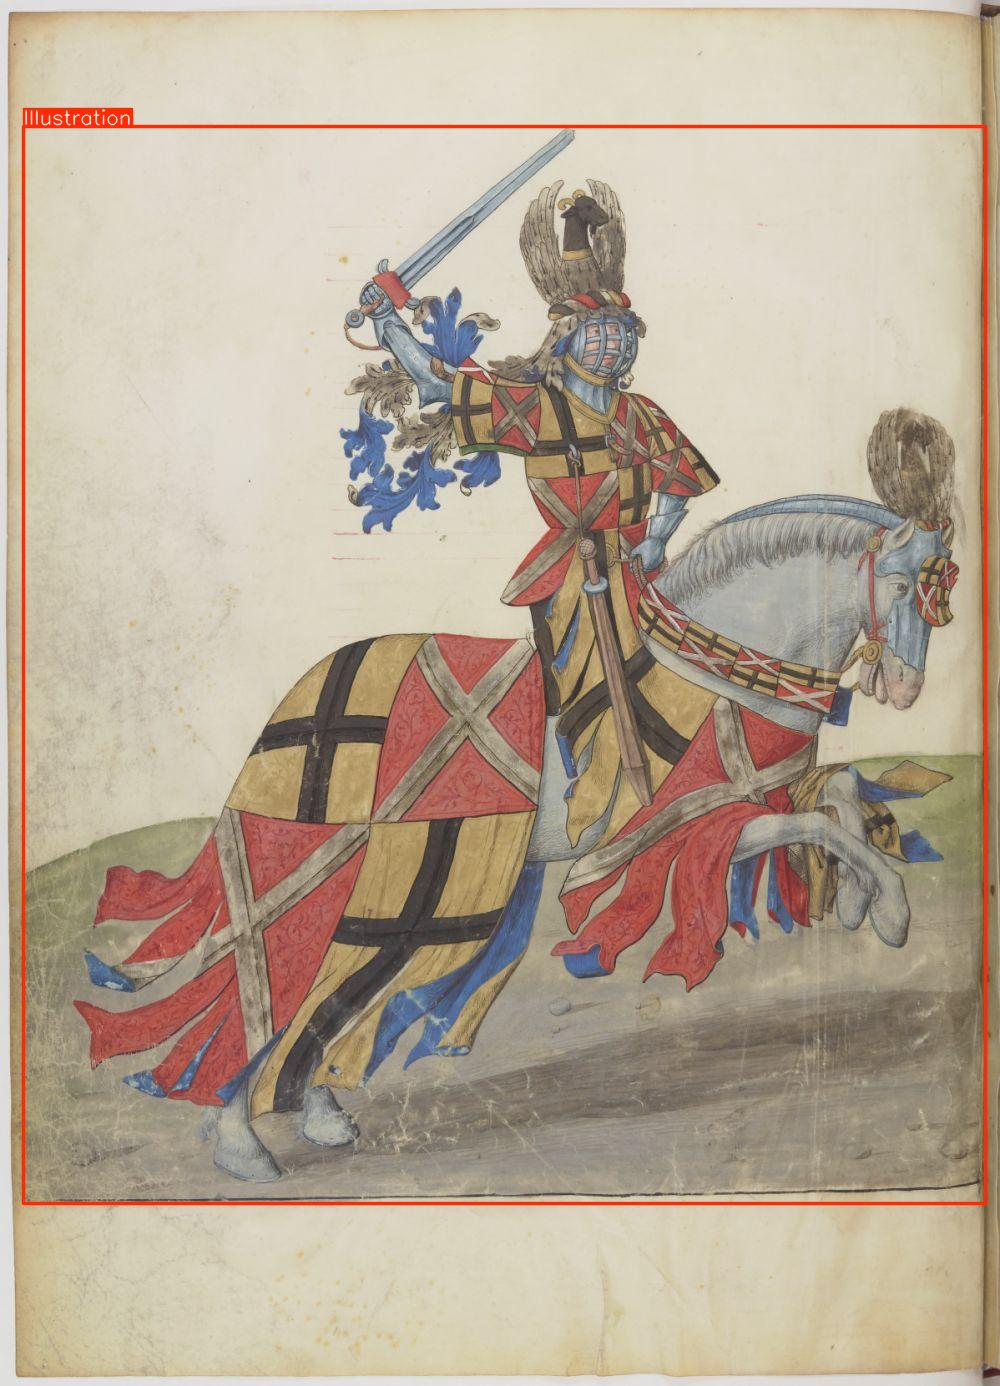
\includegraphics[scale=0.118]{img/illuhisdoc.jpg}
        \end{subfigure}
        \caption{Exemple d'une page et de son annotation en segmentation par pixel tiré du datatset IlluHisDoc.}
        \label{fig:segexemple}
\end{figure}

La complexité d'un conversion d'un dataset segmenté vient principalement de l'organisation interne des annotations. Par exemple \textit{IlluHisDoc } possède quatre classes d'annotations, mais l'organisation interne du dataset avec un dossier par classe d'annotation fait que la conversion vers des boites englobantes est relativement aisé comparé à un autre jeu de données comme \textit{SynDoc} ou chaque page peut avoir plusieurs instances segmentées de plusieurs classes différentes. La conversion d'un jeu de donnnées segmenté vers un jeu de données en boite englobante demande une réflexion sur la manière dont est construite l'annotation de segmentation au cas par cas. 

\subsection{Corriger des données}

Une fois toutes les annotations normalisées dans une ontologie et un format lisible commun, nous nous sommes concentré sur la tache de correction et d'enrichissement des données de GenHisDoc. C'est le moment où nous avons également d\^u intégrer un outil clef en main pour gérer les collections des documents à réannoter (des paquets de 1000 images et annotations), avoir un environnement graphique de travail (trancer les bo\^ites englobantes, les corriger, utiliser des fonctions de zoom, enregistrer les modifications), et également pouvoir exporter les annotations corrigées. Pour cela nous avons choisi d'utiliser la version gratuite de l'application \textit{Label Studio}.  

\subsubsection{L'environnement technique de correction : Label Studio}

\textit{Label Studio} est une application d'annotation de données développée par l'entreprise \textit{HumanSignal} et mis à disposition gratuitement en open-source dans une version limitée. L'application étant multimodale, elle possède son propre format d'annotation interne : le \textit{JSON Task}. 

\begin{figure}[h]
    \centering
    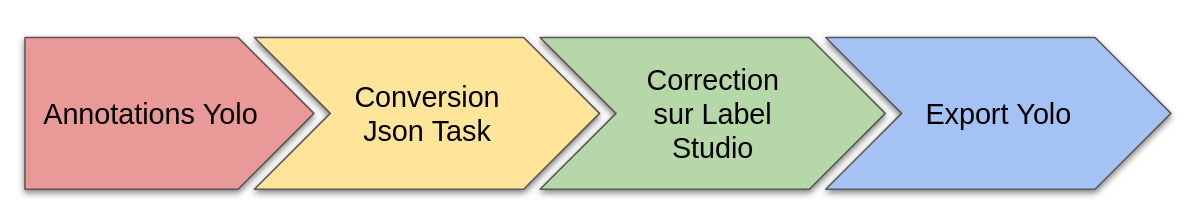
\includegraphics[scale=0.5]{img/LabelsStudio.png}
    \caption{Pipeline des tâches et conversion de format pour l'utilisation de Label Studio}
    \label{fig:LabelStudio}
\end{figure}

Label Studio prend \og techniquement \fg~en charge la conversion automatique du format YOLO vers le JSON Task ; cependant, la documentation mise à disposition est difficile d'utilisation et ignore certaines étapes intermédiaires pour pouvoir importer un projet\footnote{Label Studio Guide, \og Tutorial: Importing Local YOLO Pre-Annotated Images to Label Studio \fg, URL : \href{https://labelstud.io/blog/tutorial-importing-local-yolo-pre-annotated-images-to-label-studio/}{lien vers le blog}}. Nous avons donc réécrit et complété le tutoriel pour simplifier le travail de l'équipe qui voudrait réintégrer et corriger GenHisDoc à leurs travaux\footnote{Jules Musquin, \og Label Studio Reannotation \fg, dans \textit{GenHisDoc\_Lab} sur \href{https://github.com/Anarchiviste/GenHisDoc_Lab/blob/main/labelstudio_reannotation.md}{GitHub}}.

L'un des avantages de Label Studio tient par sa capacité à proposer un environnement applicatif modulaire pour les t\^aches d'annotations qui utilise un pseudo-langage pour sa mise en place. Cela permet de donner un bloc de code à copier-coller de la documentation aux paramètres de la tache d'annotation pour importer toute l'interface et l'ontologie à utiliser. 

\subsubsection{Corriger des annotations}

\begin{figure}[htbp]
\centering
\begin{tikzpicture}
\begin{axis}[
    ybar,
    enlargelimits=0.15,
    ylabel={Nombre d'annotations},
    symbolic x coords={Illustration, Initial, Ornament, Stamp, Table},
    xtick={Illustration, Initial, Ornament, Stamp, Table},
    nodes near coords, % Affiche les valeurs au-dessus des barres
    nodes near coords align={vertical},
    x tick label style={rotate=0, anchor=north, font=\small\bfseries},
    y tick label style={font=\small},
    ymin=0, ymax=6500,
    bar width=22pt,
    height=7cm,
    width=11cm,
    grid=major,
    grid style={dashed, gray!30},
    title={\textbf{GenHisDoc classes distribution} \\ {\small Total files: 8758 $|$ Total labels: 15976}},
    title style={align=center}
]

\addplot[fill=blue, draw=blue!70!black, bar shift=0pt] coordinates {(Illustration, 5621)};
\addplot[fill=orange, draw=orange!70!black, bar shift=0pt] coordinates {(Initial, 4650)};
\addplot[fill=green!60!black, draw=green!40!black, bar shift=0pt] coordinates {(Ornament, 3581)};
\addplot[fill=red, draw=red!70!black, bar shift=0pt] coordinates {(Stamp, 1107)};
\addplot[fill=violet, draw=violet!70!black, bar shift=0pt] coordinates {(Table, 1017)};

\end{axis}
\end{tikzpicture}
\caption{Distribution des annotations par classe dans le dataset GenHisDoc.}
\label{fig:GenHisDocDistribution}
\end{figure}

La tache de correction des annotations présente plusieurs cas de figure plus ou moins long à prendre en compte lors de la présentation de la tache aux annotateur\pmm ices.

\begin{description}
    \item[La correction géométrique :] Un modèle de détection dans Aikon a correctement identifié la présence d'une illustration. Cependant, la boîte englobante est mal tracée et demande à être réajustée. 

    \item[La correction ontologique :] Dans S-VED, les \textit{Illustration} et les \textit{Printer's Mark} étaient annotées de manière séparées. Il faut donc que le correcteur réassigne le bon label à des boîtes englobantes déjà correctement tracées. 

    \item[L'ajout d'annotations manquantes (faux négatifs) :] Les modèles automatiques ou les corpus d'origine oublient fréquemment certains objets visuels (par exemple des lettrines de petite taille ou des éléments marginaux). L'annotateur doit alors tracer manuellement les boîtes englobantes absentes de la vérité terrain initiale.

    Certains jeux de données possèdent également des images avec des éléments qui nous intéressent (pour nous essentiellement les tables) sans les annoter. L'annotateur doit donc enrichir une annotation en rajoutant les éléments qui ne faisaient pas parti de l'ontologie du jeu de données d'origine. 

    \item[La suppression des prédictions erronées (faux positifs) :] Les algorithmes détectent parfois du bruit, des taches d'encre ou des artefacts de numérisation qu'ils interprètent à tort comme des zones d'intérêt. Ces boîtes invalides doivent être retirées du jeu de données.

    \item[Le découpage ou la fusion de zones complexes :] Dans certains cas d'enluminures ou d'ornements imbriqués, l'outil initial a regroupé plusieurs éléments distincts au sein d'une unique grande boîte, ou au contraire a morcelé une illustration continue. Le correcteur doit scinder ou fusionner ces zones pour respecter les granularités fixées par l'ontologie GenHisDoc. C'est de loin la t\^ache de correction la plus longue et éprouvante. 
\end{description}
\chapter[Entraîner et évaluer]{Entraîner et évaluer un modèle}

\lettrine{A}{fin de valider} la rigueur de notre jeu de données et la pertinence de notre schéma d'annotation, l'aboutissement de ce travail réside dans la conversion de la vérité terrain en une capacité d'inférence sur des corpus inédits. C'est en effet à travers l'épreuve de l'entraînement que la modélisation conceptuelle se traduit en un outil opérationnel pour l'analyse documentaire.

Ce chapitre retrace l'ensemble du protocole expérimental, de l'entraînement à l'évaluation du modèle. Nous détaillerons d'abord la configuration des hyperparamètres, ces derniers leviers sur lesquels nous pouvons agir pour optimiser l'efficacité ou les performances du modèle. Nous analyserons ensuite les résultats obtenus à l'aune des métriques de détection, en confrontant les indicateurs statistiques aux exigences concrètes du dépouillement historique. Enfin, nous étudierons les principales erreurs de prédiction afin de dégager des pistes d'amélioration ciblées, envisageant l'évaluation non pas comme un terme définitif, mais comme le moteur d'une démarche itérative.

\section{Les hyperparamètres}

Les hyperparamètres sont les variables de configuration fixées par l'expérimentateur avant le lancement de l'entraînement. Contrairement aux paramètres (les poids et biais du réseau de neurones), qui sont appris et ajustés automatiquement par rétropropagation du gradient, les hyperparamètres pilotent la dynamique de l'apprentissage et définissent le cadre structurel dans lequel le modèle évolue.

La performance d'un algorithme de vision par ordinateur dépend de sa capacité à généraliser ses inférences sur des documents d'un type différent de ses documents d'entraînement. Cette capacité de généralisation désigne l'aptitude d'un modèle à maintenir de bonnes performances sur des images inédites, au-delà de son seul corpus d'apprentissage. À l'inverse, l'écueil principal de l'entraînement réside dans le surapprentissage (\textit{overfitting}) : le réseau mémorise alors les bruits et les spécificités propres aux données d'origine au lieu d'en extraire des caractéristiques visuelles réellement représentatives. Le contrôle de ces hyperparamètres conditionne la capacité du réseau à extraire des motifs abstraits, à gérer les variations d'échelle et à généraliser sur de nouvelles sources sans tomber dans le piège du surapprentissage.
Les hyperparamètres structurants en vision par ordinateur s'articulent autour de quatre grands axes :

\begin{description}
	\item[Dimensionnement de l'entrée et charge mémoire :]\hfill
	\begin{itemize}
		\item \textbf{Taille de l'image :} Définit la résolution spatiale des images fournies au réseau (par exemple $640 \times 640$ pixels). Une résolution élevée est essentielle pour détecter des objets de petite taille ou préserver les détails fins d'une mise en page, mais elle augmente de manière quadratique l'empreinte en mémoire VRAM et les temps de calcul.
		\item \textbf{Taille de lot (\textit{Batch Size}) :} Une taille de lot importante ($32$ ou $64$ images) permet au modèle de dégager une tendance générale très stable, puisqu'il tire ses enseignements d'un large échantillon d'un seul coup. À l'inverse, un lot réduit ($8$ ou $16$ images) oblige le modèle à s'ajuster plus fréquemment, sur la base de très peu d'exemples. Cet apprentissage, qui devient alors volontairement plus instable, peut être utilisé comme un garde-fou : il empêche la machine de s'enfermer dans de fausses déductions, par exemple, se convaincre qu'une tâche d'humidité récurrente est une illustration. Traiter les images par petits groupes force ainsi le modèle à rester adaptable face à la grande hétérogénéité matérielle des documents.
	\end{itemize}
	
	\item[Optimisation et dynamique d'apprentissage :]\hfill
	\begin{itemize}
		\item \textbf{Le taux d'apprentissage initial (\textit{Learning Rate} - $lr$) :} Il détermine l'ampleur des corrections que le modèle s'applique à lui-même lorsqu'il identifie une erreur. Un taux trop fort pousse le modèle à réagir de manière excessive (techniquement, on parle de \og divergence de la fonction de perte \/\textit{loss function}\/ \fg) ; dans les faits, le modèle n'arrive plus à stabiliser ses poids ni à progresser continuellement en raison de la trop grande volatilité de ses prédictions. À l'inverse, un taux trop faible rend le modèle excessivement timide dans ses déductions, ce qui conduit à une stagnation prématurée de son apprentissage.
		\item \textbf{La planification du taux d'apprentissage (\textit{LR Scheduler}) :} Elle adapte la cadence du modèle tout au long de son entraînement. Le réseau commence par apprendre rapidement pour dégager la structure globale des documents, puis réduit progressivement l'ampleur de ses corrections. Une volatilité élevée au début lui permet de découvrir la structure des documents, tandis qu'une volatilité basse en fin d'entraînement permet de consolider les acquis.
		\item \textbf{La décroissance des poids (\textit{Weight Decay}) :} C'est une règle de régularisation qui empêche le modèle d'accorder une importance excessive à un détail visuel isolé. En appliquant une forme d'oubli progressif sur les pondérations du réseau, cette technique évite au modèle de sur-interpréter les particularités idiosyncratiques des données d'entraînement.
	\end{itemize}
	
	\item[L'augmentation artificielle des données :]\hfill
	En vision artificielle, la quantité et la diversité des données sont déterminantes. Les hyperparamètres d'augmentation génèrent des variations artificielles des images d'origine sans coût d'annotation supplémentaire. La plupart des bibliothèques d'entraînement appliquent automatiquement des transformations géométriques (rotations, translations, cisaillement, changements d'échelle) ainsi que des modifications colorimétriques (saturation, teintes). La bibliothèque YOLO d'Ultralytics intègre en outre des transformations plus complexes, telles que la juxtaposition de plusieurs images du jeu de données ou leur superposition à différents niveaux de transparence, permettant au modèle de développer une meilleure robustesse face à une forte densité d'éléments à détecter.
	
	\item[L'équilibrage des priorités de détection (\textit{Loss Balancing}) :]\hfill
	Lors d'une tâche d'inférence, le modèle doit réussir simultanément trois missions : repérer où se trouve un élément, déterminer sa nature et ajuster ses contours. Ce paramétrage permet de pondérer les priorités de la machine afin qu'elle ne néglige aucune de ces étapes : \hfill
	\begin{itemize}
		\item \textbf{Le repérage de la zone ($\text{Box Loss } L_{\text{box}}$) :} Il évalue la capacité du modèle à placer son cadrage au bon endroit sur la page.
		\item \textbf{L'identification de la catégorie ($\text{Class Loss } L_{\text{cls}}$) :} Il contrôle si le modèle attribue l'étiquette sémantique correcte à la zone encadrée.
		\item \textbf{La précision des bordures ($\text{DFL } L_{\text{dfl}}$) :} Il s'assure de la finesse du découpage des contours. C'est la finition qui permet au cadre de coller aux limites visuelles de l'objet à détecter, même dans des cas difficiles (flou d'impression, dégradation du papier ou chevauchement de structures).
	\end{itemize}
\end{description}

L'optimisation des hyperparamètres consiste à rechercher la meilleure combinaison de réglages pour maximiser les capacités du modèle. Dans le cadre d'un projet de vision artificielle appliquée à l'analyse documentaire, l'enjeu est d'éviter le surapprentissage en maintenant une bonne capacité de généralisation, rationaliser le temps de calcul (souvent limité sur les infrastructures de recherche), et surtout adapter correctement l'algorithme au corpus. 

\section{Évaluer les résultats de l'inférence}

\subsection{Définir la méthodologie d'évaluation}

\subsubsection{L'importance du découpage du jeu de données (\textit{Data Splitting})}

La constitution d'un jeu de données repose sur la répartition des documents en trois sous-ensembles hermétiques : l'entraînement (\textit{train}), la validation (\textit{val}) et le test (\textit{test}). Le premier sert à l'ajustement direct des poids du réseau, tandis que le second permet d'évaluer la progression au fil des époques et de guider l'ajustement des hyperparamètres. Le jeu de test, quant à lui, doit être mis de côté et rester totalement inédit pour le modèle jusqu'à l'évaluation finale. Isolé de la phase de développement, il évite d'adapter implicitement la configuration du modèle aux spécificités de ce corpus d'évaluation. Cette séparation stricte constitue la seule garantie méthodologique d'une mesure objective de la capacité de généralisation de l'algorithme.

Idéalement, il faut répartir les données par manuscrit d'origine, et non par échantillonnage : si le jeu de données contient des pages issues de plusieurs documents, il faut distribuer des documents entiers entre les ensembles d'entraînement, de validation et de test, et jamais des pages individuelles d'un même document. Sinon, le modèle peut \og reconnaître \fg le style graphique, le papier ou les motifs récurrents d'un manuscrit vu en entraînement, ce qui gonfle artificiellement les scores de test. C'est cependant ce qui a été fait pour l'évaluation des modèles entraînés sur GenHisDoc, l'ayant réalisé après l'entraînement sans possibilité de corriger cette erreur faute de temps. Il faut également tenter d'éviter la présence de quasi-doublons entre le jeu de données d'entraînement et le jeu de données de test, certains sous-corpora utilisés dans GenHisDoc possédant de nombreux quasi-doublons, comme S-VED ou Horae. La définition du quasi-doublon s'avère par ailleurs très délicate à formaliser (deux images pouvant apparaître similaires à un humain alors que cela n'handicape pas l'entraînement du modèle, et inversement).

\subsubsection{La représentativité de la distribution réelle}

Idéalement, le jeu de test doit refléter les conditions d'usage réel du modèle, et non pas seulement la distribution du jeu d'entraînement :

\begin{itemize}
	\item \textbf{Diversité des sources :} prise en compte des différentes périodes historiques, des types de documents variés, ainsi que des dégradations et des défauts de numérisation.
	
	\item \textbf{Diversité des classes :} représentation suffisante de toutes les catégories d'intérêt — en veillant à la problématique de la distribution à queue longue —, un jeu de test dominé par la classe majoritaire risquant de masquer les faiblesses sur les cas minoritaires.
\end{itemize}

De surcroît, la constitution du jeu de test doit être stratifiée selon les classes, les types de documents et, de préférence, la difficulté (la densité d'objets par page). Avec un total de plus de 8\,000 images, notre jeu de test compte environ 900 images et plus de 1\,600 vérités terrain (GT), ce qui est suffisant pour garantir que l'ensemble des classes de GenHisDoc est correctement représenté.

\subsection{Résultats pour GenHisDoc}

Il s'agit de jauger le compromis fondamental entre l'exhaustivité de la recherche (le rappel) et la fiabilité des détections restituées (la précision). Pour apprécier ces performances en situation réelle, les résultats obtenus par notre modèle entraîné sur GenHisDoc sont confrontés à ceux du modèle historiquement déployé au sein de l'application AIKON, à l'aune des indicateurs statistiques détaillés dans le tableau~\ref{tab:GenHisDocYolo}.

\subsubsection{Comprendre les métriques générales}

Les résultats témoignent d'un niveau de performance élevé et homogène du modèle GenHisDoc, aussi bien sur la classe \textit{Illustration} que sur l'ensemble des classes du schéma d'annotation. Le score AP@50 atteint $87{,}87\,\%$ pour la seule classe \textit{Illustration} et se maintient à un niveau comparable ($84{,}04\,\%$) lorsque l'ensemble des classes est pris en compte, malgré un volume de vérités terrain nettement supérieur ($1\,659$ occurrences contre $558$) et, par conséquent, une tâche de discrimination plus exigeante. Cette stabilité suggère que le modèle ne doit pas sa performance à une spécialisation étroite sur un type d'objet visuel particulier, mais qu'il généralise correctement à la diversité des éléments à détecter dans les documents historiques. La précision et le rappel restent tous deux élevés et proches l'un de l'autre, tant pour la classe \textit{Illustration} ($0{,}8623$ et $0{,}8978$) que toutes classes confondues ($0{,}8473$ et $0{,}8728$), ce qui traduit un compromis équilibré entre l'exhaustivité de la détection et la fiabilité des résultats restitués, plutôt qu'une optimisation artificielle d'une métrique au détriment de l'autre. Les scores $F_1$ qui en résultent ($0{,}8797$ et $0{,}8599$ respectivement) confirment la robustesse de cet équilibre.

L'IoU moyen des détections, supérieur à $0{,}85$ dans les deux configurations et atteignant $0{,}9033$ sur la seule classe \textit{Illustration}, indique par ailleurs une excellente qualité de localisation des boîtes englobantes, et non une simple justesse de classification : les objets détectés le sont avec un niveau de précision spatiale élevé, ce qui s'avère particulièrement crucial pour des tâches avales (\textit{downstream tasks}) comme l'extraction ou le recadrage automatique d'illustrations. Enfin, si la comparaison avec le modèle AIKON historiquement en production enrichit l'analyse, la possibilité d'une évaluation strictement monoclasse (\textit{Illustration} contre \textit{Illustration}) constitue un point méthodologique notable, dans la mesure où elle permet d'isoler la contribution du nouveau modèle et du corpus GenHisDoc indépendamment de l'élargissement du périmètre ontologique.

\begin{table}[htbp]
	\centering
	\ra{1.25}
	\caption{Comparaison des résultats d'évaluation entre GenHisDoc et Aikon. GenHisDoc est un yolo 26 large entraîné sur le dataset GenHisDoc produit durant le stage. Aikon est un yolo 5 large entraîné d'abord sur les diagrammes puis finetuné pour détecter plus généralement toutes les illustrations. C'est le modèle qui équipe actuellement Aikon.}
	\begin{tabular}{lccc}
		\toprule
		& \multicolumn{2}{c}{\textbf{GenHisDoc}} & \textbf{Aikon} \\
		\cmidrule(r){2-3} \cmidrule(l){4-4}
		\textbf{Métrique / Indicateur} & \textbf{Illustration} & \textbf{Toutes classes} & \textbf{Illustration} \\
		\midrule
		\multicolumn{4}{l}{\textit{Données de test et Détection}} \\
		\hspace{1em} Fichiers traités & 876 & 876 & 876 \\
		\hspace{1em} Nombre total de GT & 558 & 1659 & 558 \\
		\hspace{1em} IoU Moyen (Détections) & 0,9033 & 0,8595 & 0,8762 \\
		\midrule
		\multicolumn{4}{l}{\textit{Performance globale}} \\
		\hspace{1em} AP@50 (mAP@50) & \textbf{ 0,8787 (87,87\%)} & 0,8404 (84,04\%) & 0,4815 (48,15\%) \\
		\midrule
		\multicolumn{4}{l}{\textit{Métriques au seuil fixe ($\ge$ 0,25)}} \\
		\hspace{1em} Vrais Positifs (TP) & 501 & 1448 & 355 \\
		\hspace{1em} Faux Positifs (FP) & 80 & 261 & 208 \\
		\hspace{1em} Faux Négatifs (FN) & 57 & 211 & 203 \\
		\hspace{1em} Précision & 0,8623 & 0,8473 & 0,6306 \\
		\hspace{1em} Rappel (Recall) & 0,8978 & 0,8728 & 0,6362 \\
		\hspace{1em} Score F1 & \textbf{0,8797} & 0,8599 & 0,6334 \\
		\bottomrule
	\end{tabular}
	\label{tab:GenHisDocYolo}
\end{table}
\subsubsection{Comprendre les métriques par classes}

\begin{figure}[h]
	\centering
	\begin{subfigure}{0.48\textwidth}
		\centering
		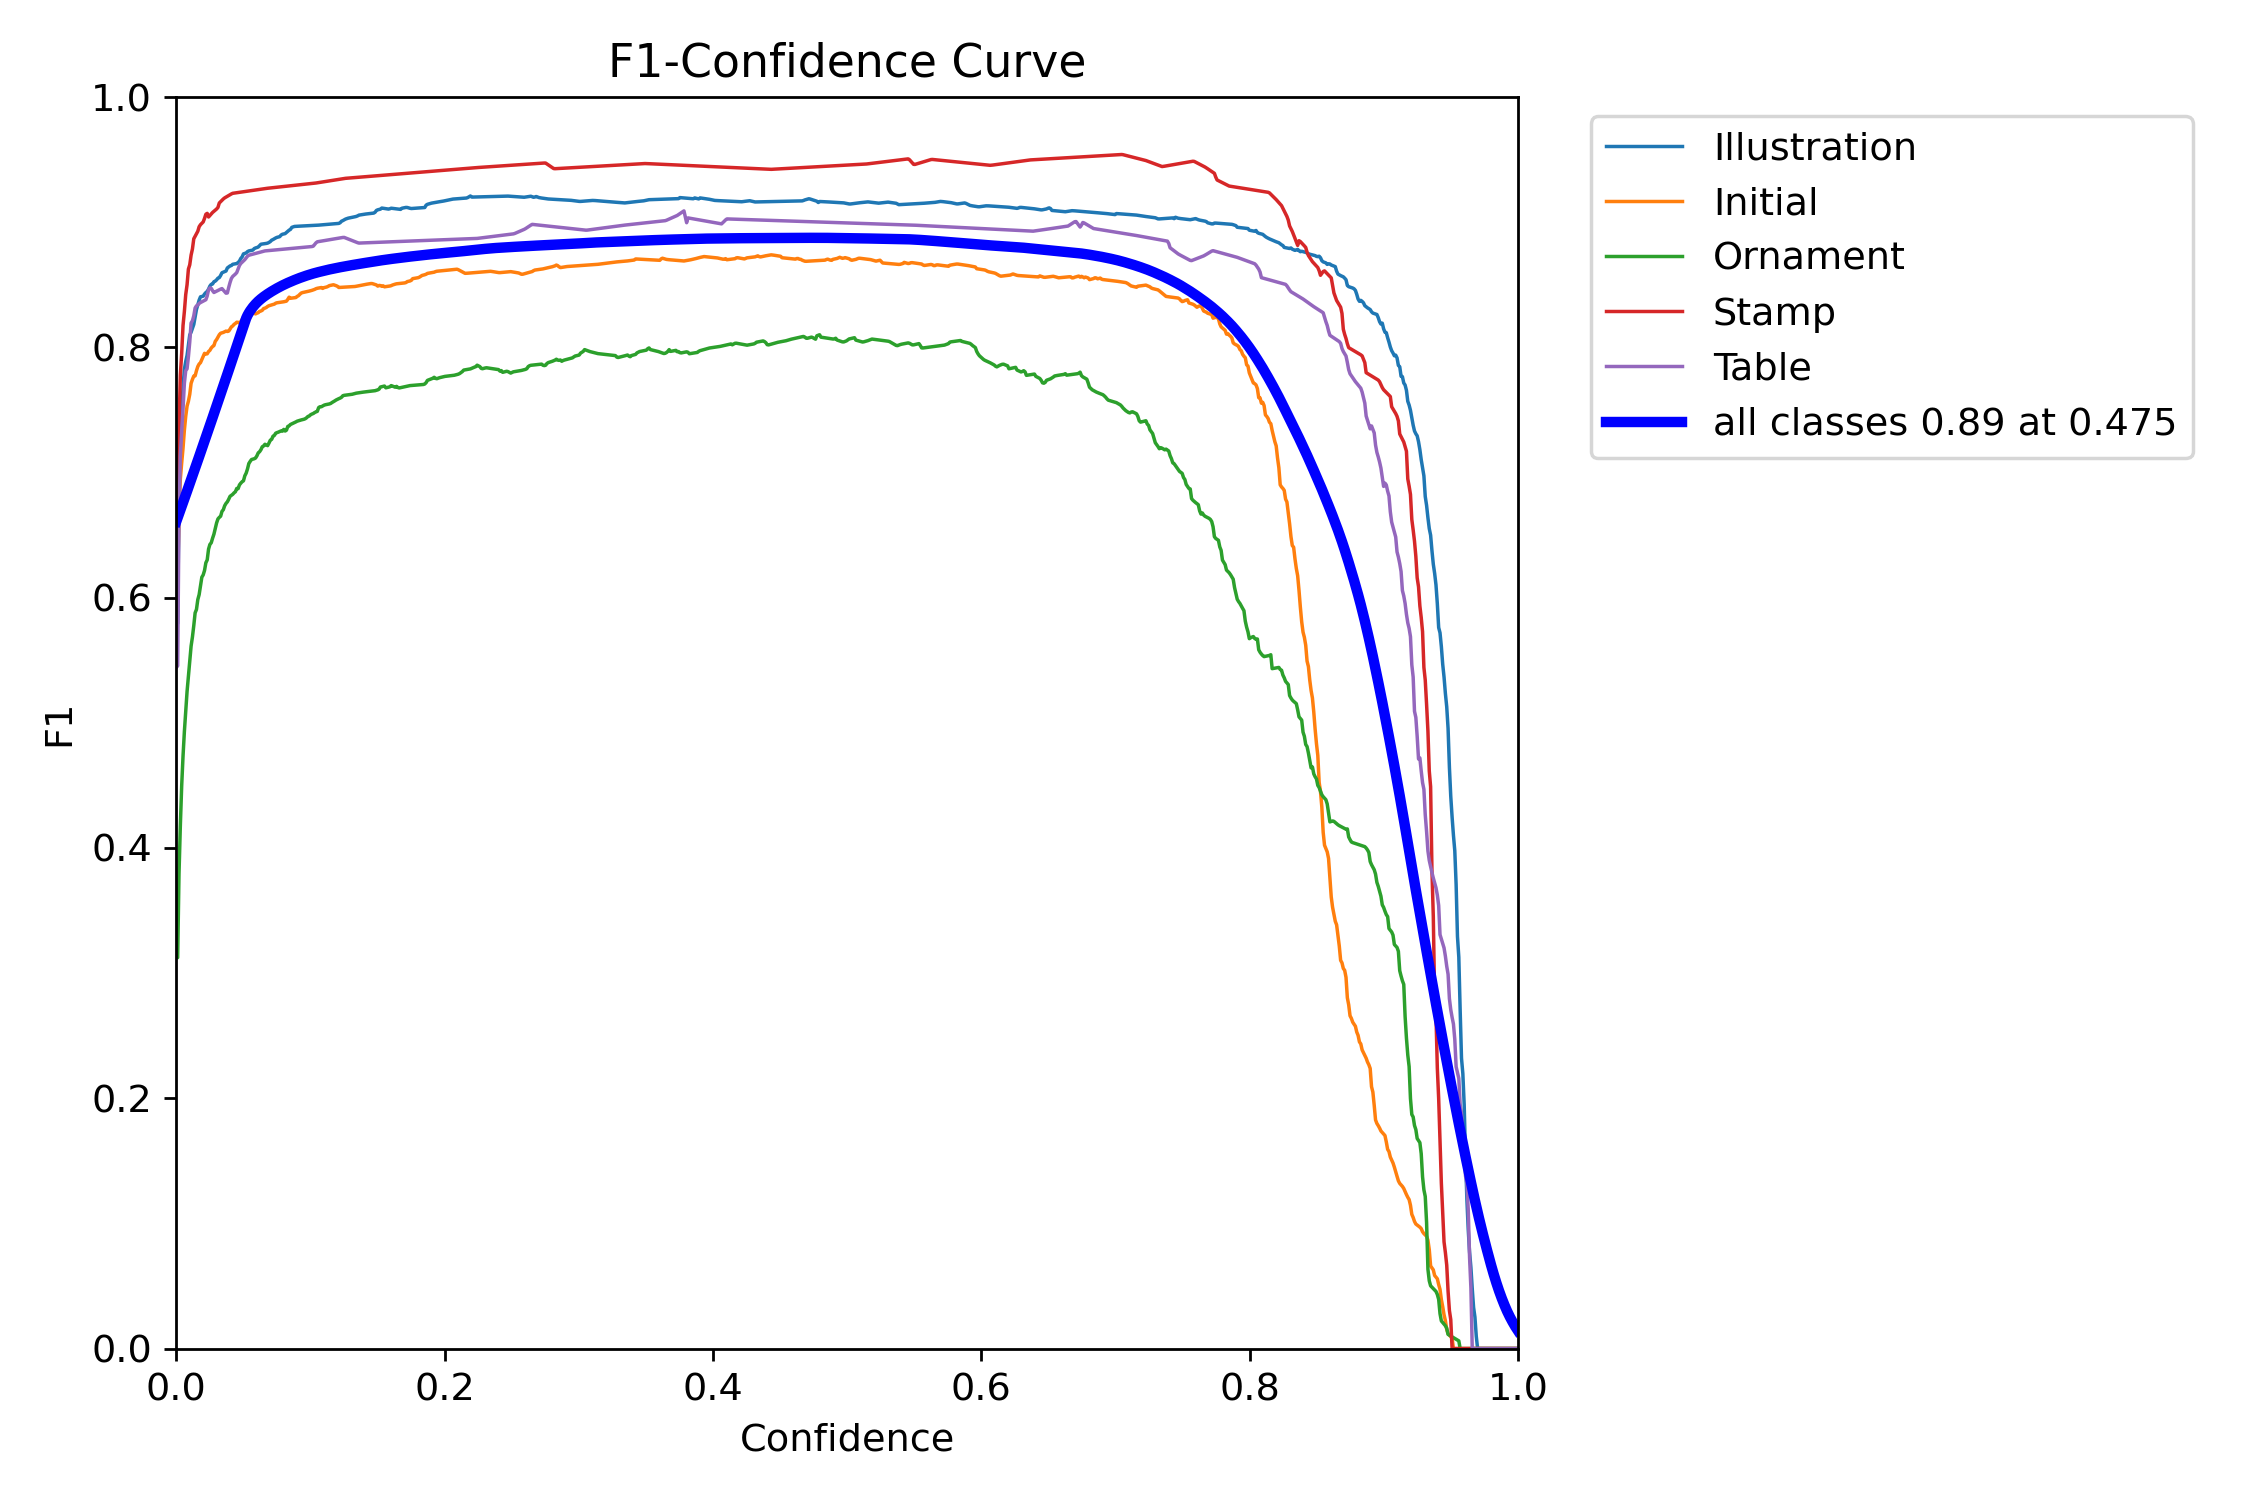
\includegraphics[width=\linewidth, height=8cm, keepaspectratio]{img/BoxF1_curve.png}
		\caption{Score $F_1$}
		\label{fig:f1score}
	\end{subfigure}
	\hfill
	\begin{subfigure}{0.48\textwidth}
		\centering
		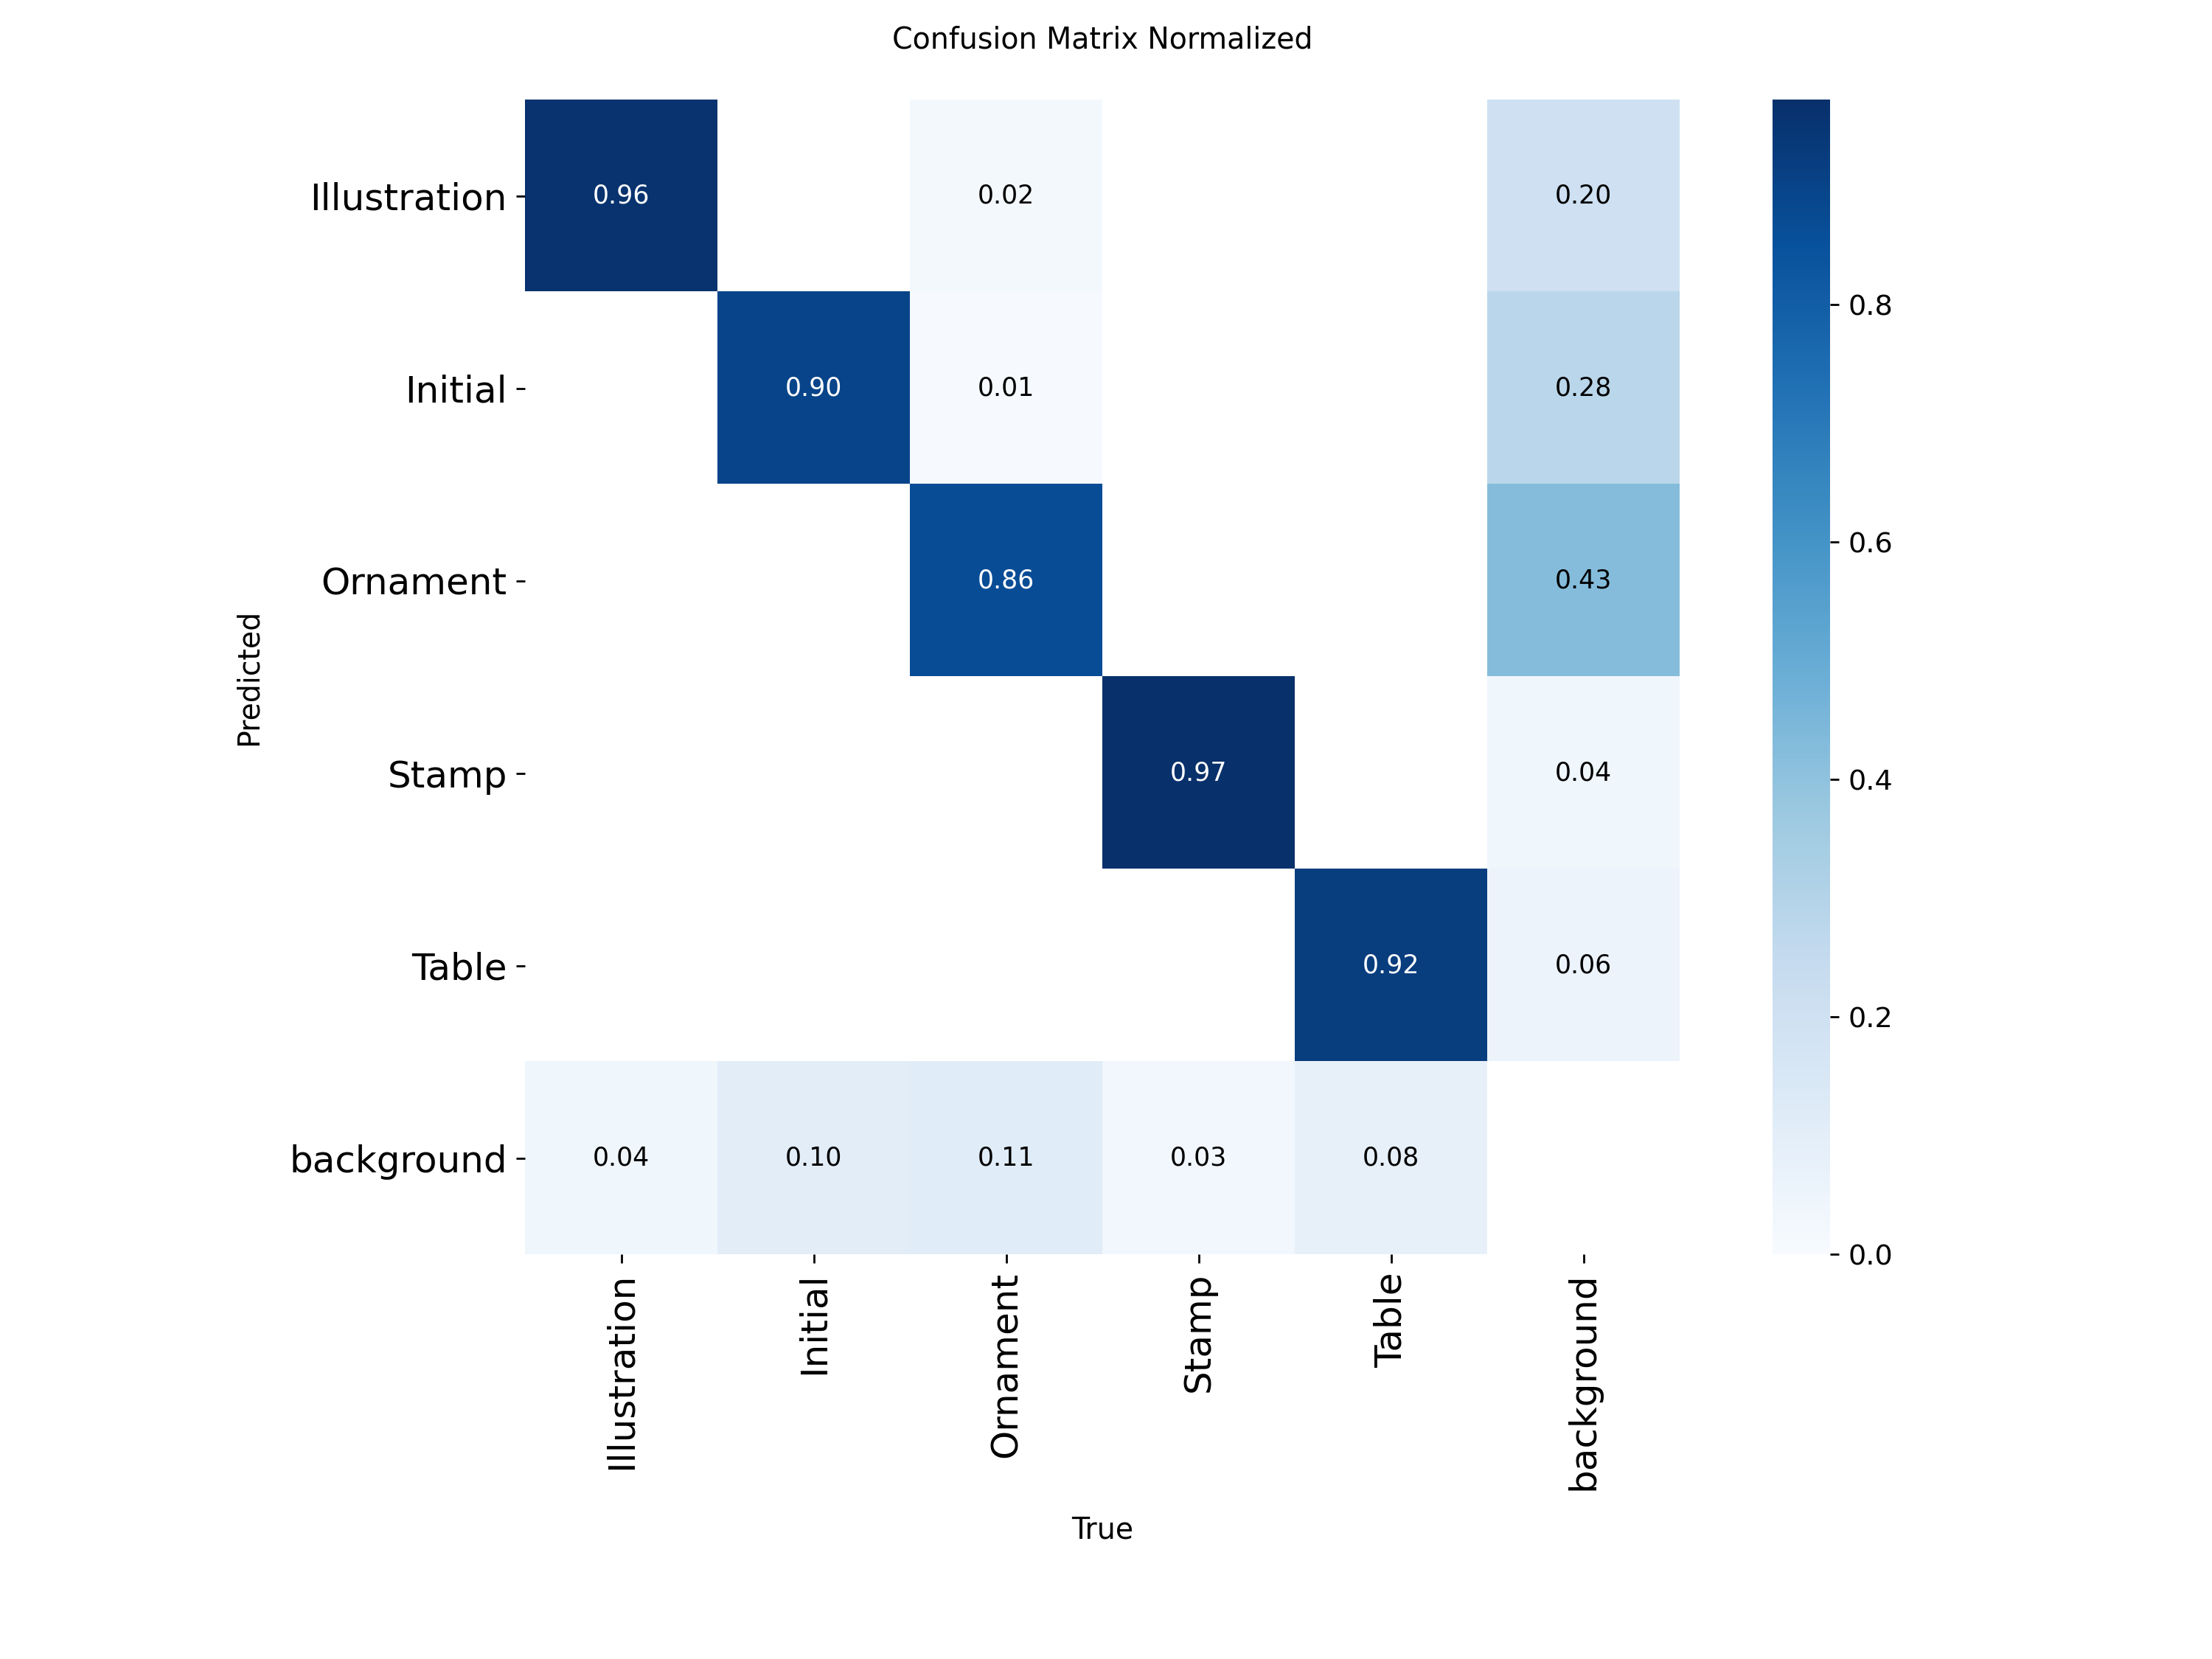
\includegraphics[width=\linewidth, height=8cm, keepaspectratio]{img/confusion_matrix_normalized.png}
		\caption{Matrice de confusion normalisée}
		\label{fig:confusionmatrix}
	\end{subfigure}
	\caption{Représentation des scores $F_1$ et de la matrice de confusion normalisée des classes du modèle entraîné sur GenHisDoc.}
	\label{fig:confusionF1}
\end{figure}

{\raggedright\textbf{Le score $F_1$ par classes :}}
\begin{itemize}
	\item \textbf{\textit{Stamp}} (en rouge) est la classe la plus performante, affichant un plateau proche de $0{,}95$ sur une plage de confiance très large (jusqu'à environ $0{,}7$). Ce résultat s'explique par la nature de l'objet, visuellement homogène et hautement discriminant (formes géométriques régulières et contrastes marqués).
	
	\item \textbf{\textit{Illustration}} (en bleu) et \textbf{\textit{Table}} (en violet) se comportent de manière satisfaisante, avec des scores oscillant entre $0{,}88$ et $0{,}92$, en adéquation avec l'agrégat global. L'efficacité de la détection des tableaux constitue l'une des surprises notables de ce travail : alors que cette classe pouvait initialement paraître difficile à circonscrire en raison de sa variabilité typographique, l'homogénéité des principes d'annotation a permis au modèle de la modéliser avec succès.
	
	\item \textbf{\textit{Initial}} (en orange) se situe en retrait, autour de $0{,}85\text{--}0{,}87$, avec un déclin de performance qui s'amorce plus précocement (vers $0{,}6$ de confiance) que pour les autres catégories. Le modèle manifeste ici une moindre certitude, imputable soit à une forte hétérogénéité visuelle (les lettrines historiques adoptant des styles extrêmement variés), soit à des imprécisions dans les consignes d'annotation, soit encore à la présence d'éléments parasites morphologiquement proches, tels que les pieds-de-mouche (\textit{pilcrows}, $\P$).
	
	\item \textbf{\textit{Ornament}} (en vert) constitue la classe la plus fragile, plafonnant à environ $0{,}80$ avec une décroissance marquée dès $0{,}5\text{--}0{,}6$ de confiance. Cette faiblesse témoigne de la difficulté inhérente à la détection de cette catégorie, caractérisée par une forte variabilité intra-classe (les ornements typographiques et encadrements historiques revêtant des formes d'une grande hétérogénéité).
\end{itemize}

{\raggedright\textbf{La matrice de confusion normalisée :}}

Chaque colonne correspond à une classe réelle (\textit{True}) et répartit le devenir de tous les objets réels de cette catégorie entre les différentes prédictions possibles. La ligne \og \textit{background} \fg, située en bas, indique la proportion d'objets réels manqués (faux négatifs, prédits comme une absence d'objet). La colonne \og \textit{background} \fg, située à droite, fonctionne différemment : elle répartit l'ensemble des fausses détections (prédictions sans objet réel correspondant, ou faux positifs) entre les classes prédites à tort.

\begin{table}[h]
	\centering
	\ra{1.25}
	\begin{tabular}{lcc}
		\toprule
		\textbf{Classe} & \textbf{Bien détecté} & \textbf{Manqué} ($\text{FN} \to \text{Background}$) \\
		\midrule
		\textit{Stamp} & $0{,}97$ & $0{,}03$ \\
		\textit{Illustration} & $0{,}96$ & $0{,}04$ \\
		\textit{Table} & $0{,}92$ & $0{,}08$ \\
		\textit{Initial} & $0{,}90$ & $0{,}10$ \\
		\textbf{\textit{Ornament}} & \textbf{0{,}86} & \textbf{0{,}11 (+ 0{,}03 mal classé)} \\
		\bottomrule
	\end{tabular}
	\caption{Extraction des taux de détection et des faux négatifs par classe issus de la matrice de confusion normalisée.}
	\label{tab:matrice}
\end{table}

La classe \textit{Ornament} s'avère bien la plus fragile, affichant le taux de rappel le plus faible et se révélant être la seule à présenter des confusions inter-classes non négligeables : $2\,\%$ des \textit{Ornament} réels sont prédits à tort comme des illustrations, et $1\,\%$ comme des lettrines. Cette porosité est cohérente d'un point de vue codicologique, les ornements typographiques et encadrements se rapprochant parfois visuellement de motifs décoratifs d'illustrations ou de lettrines historiées, ce qui complexifie leur distinction par le modèle.

Nous avions également ajouté un système de découpage des lettrines trop complexes, dissociant l'espace de la lettre, considéré comme une lettrine, et l'espace de son ornementation, considéré comme un ornement. Ce système, hérité du corpus Horae, permet de limiter le bruit pour les lettrines immenses qui occupent la moitié d'une page.

L'analyse de la matrice de confusion révèle en outre que la classe \textit{Ornament} concentre à elle seule $43\,\%$ de l'ensemble des fausses détections du modèle (contre $28\,\%$ pour \textit{Initial}, $20\,\%$ pour \textit{Illustration}, $6\,\%$ pour \textit{Table} et seulement $4\,\%$ pour \textit{Stamp}). Autrement dit, lorsque le modèle \og hallucine \fg{} un objet inexistant, il s'agit le plus souvent d'un ornement.

\section{Les pistes d'amélioration}

Les premiers résultats obtenus sur GenHisDoc, aussi encourageants soient-ils dans l'ensemble, mettent en évidence certaines limites qu'il convient d'interroger avant d'envisager une simple poursuite de l'entraînement. Nous devons reconsidérer en partie, au-delà du seul réglage technique du modèle, la pertinence des choix méthodologiques opérés en amont, qu'il s'agisse de la constitution du corpus, de la définition des classes, ou de l'adéquation de l'approche retenue avec les besoins spécifiques de l'analyse de documents historiques. C'est cette mise en tension entre les résultats observés et les choix initiaux qui doit guider la définition des axes d'amélioration à privilégier.

Nous détaillons dans cette section les différentes approches testées ainsi que leurs résultats respectifs.

\subsection{Modifier les hyperparamètres}

Le réglage des hyperparamètres constitue le levier d'amélioration le plus immédiat, dans la mesure où il n'implique de revenir ni sur les annotations ni sur la définition des classes : il s'agit d'optimiser la manière dont le modèle apprend. Cet axe est aussi celui pour lequel les courbes de perte et de convergence, déjà présentées, offrent le diagnostic le plus direct, en révélant d'éventuels signes de sous-apprentissage, de surapprentissage ou une durée d'entraînement mal calibrée.

Les modèles que nous avons entraînés sur GenHisDoc obéissaient tous aux mêmes hyperparamètres ($640 \times 640$ pixels en taille d'image, $100$ époques d'entraînement, paramètres par défaut pour le reste des hyperparamètres).

L'examen conjoint des pertes d'entraînement et de validation (figure~\ref{fig:losses}) constitue le point le plus instructif du point de vue du réglage des hyperparamètres. Si les deux courbes décroissent de concert jusqu'aux alentours de l'époque $60$, un écart croissant apparaît ensuite entre la perte de classification d'entraînement, qui continue de chuter fortement, et son homologue de validation, qui se stabilise puis stagne autour de $0{,}5$ à partir de l'époque $70$ : ce découplage constitue un indice classique de début de surapprentissage, contenu néanmoins par le fait que les métriques de validation (précision, rappel, $\text{mAP}_{50}$, $\text{mAP}_{50\text{--}95}$) n'accusent pas de dégradation correspondante et se maintiennent sur un plateau élevé entre les époques $70$ et $100$. Le plateau atteint dès l'époque $70$ pour la $\text{mAP}_{50}$ ($\approx 0{,}91$) et la poursuite d'une lente progression de la $\text{mAP}_{50\text{--}95}$ (de $0{,}69$ à $0{,}70$) jusqu'aux époques $72\text{--}83$ indiquent que la durée d'entraînement de $100$ époques était globalement bien calibrée, sans marge de progression significative résiduelle, et qu'un arrêt anticipé (\textit{early stopping}) autour des époques $70\text{--}80$ aurait vraisemblablement permis d'obtenir des performances quasi identiques à un coût de calcul moindre.

\begin{figure}[h]
	\centering
	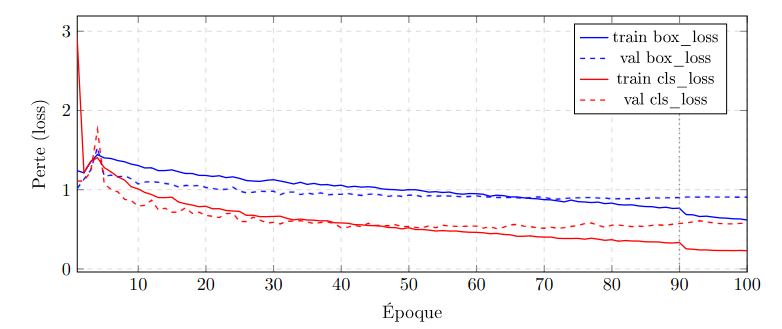
\includegraphics[width=0.8\textwidth]{img/loss.png}
	\caption{Comparaison des pertes d'entraînement et de validation (\textit{box loss} et \textit{classification loss}).}
	\label{fig:losses}
\end{figure}

\subsection{Mettre en place une meilleure méthodologie d'évaluation}

La pertinence des indicateurs statistiques présentés précédemment dépend directement de la rigueur avec laquelle le jeu de données d'évaluation est constitué.

Corriger les biais méthodologiques identifiés précédemment afin d'obtenir un jeu de test et de validation parfaitement sain constitue un enjeu majeur pour l'évolution du projet. Un découpage strict, opéré par manuscrits distincts et expurgé de tout quasi-doublon, permet d'abord d'obtenir des métriques beaucoup plus fidèles et réalistes quant aux performances de l'algorithme en conditions réelles de dépouillement. L'analyse de ces erreurs, désormais affranchie de toute fuite de données, fournit en aval des informations précieuses pour cibler les corrections à apporter (ajustement de l'ontologie, ajout de documents spécifiques pour combler un manque, modification des hyperparamètres). L'évaluation ne s'apparente plus alors à un simple constat, mais devient un véritable levier d'amélioration continue.

\subsection{Modifier et faire évoluer les annotations}

Modifier et enrichir les données au sein d'un corpus d'apprentissage constitue souvent le levier le plus déterminant pour faire progresser les performances d'un modèle de vision. C'est toutefois l'un des plus coûteux en temps et en ressources humaines, puisqu'il implique de revenir sur des phases d'annotation manuelle.

\begin{description}
	\item[La correction et la purification des annotations :] Un examen qualitatif des prédictions erronées peut révéler une insuffisance de la vérité terrain. Par exemple, dans le cas de GenHisDoc, reprendre les annotations de la classe \textit{Ornament} pour les préciser géométriquement et les corriger ontologiquement permettrait d'améliorer les performances du modèle.
	
	\item[Changer les directives d'annotation (\textit{guidelines}) :] Conserver les mêmes classes tout en précisant la manière dont les documents doivent être découpés. En uniformisant ces consignes de saisie, on réduit drastiquement la variabilité intra-classe. Le modèle bénéficie alors d'une plus grande cohérence géométrique dans ses exemples, ce qui améliore directement sa capacité à bien dimensionner ses cadres.
	
	\item[Améliorer la représentativité des classes :] Ce problème ne concerne pas directement GenHisDoc (où les volumes d'annotations suffisent à garantir un bon équilibre), mais remédier aux déséquilibres dans la distribution des classes peut avoir un effet très bénéfique sur l'entraînement d'un modèle de vision.
\end{description}

\subsection{Transformer l'ontologie}

Cette dernière solution est la plus coûteuse, car elle revient à jeter une grande partie du travail d'annotation produit, à remanier en profondeur la vérité terrain et à reprendre l'ensemble des directives d'annotation.

\begin{description}
	\item[La simplification par fusion (regroupement) :] C'est l'approche la moins destructrice pour le jeu de données. Si l'objectif final se limite à l'extraction de zones décorées, fusionner \textit{Ornament} et \textit{Illustration} en une méta-classe supprimerait mécaniquement la confusion inter-classes et ferait chuter le taux de faux positifs. Les annotations existantes sont conservées et l'on modifie seulement leur étiquette, mais au détriment de la granularité de l'analyse historique.
	
	\item[La complexification par scission (sous-spécialisation) :] À l'inverse, si l'on exige une plus grande finesse d'analyse, il convient de scinder les catégories confondues en remplaçant \textit{Ornament} par des classes visuellement plus homogènes. Le coût est ici maximal : cette approche oblige l'équipe de recherche à rouvrir des milliers de documents annotés pour reclasser, redessiner ou redéfinir les boîtes englobantes selon de nouveaux critères.
\end{description}

Dans le cadre de GenHisDoc, l'une des modifications d'ontologie pertinentes pour améliorer l'efficacité du modèle sur les ornementations consisterait peut-être à séparer les éléments manuscrits des éléments imprimés. Si l'on souhaite à terme réintégrer des corpus de presse ou des imprimés anciens au sein de GenHisDoc, une refonte encore plus profonde de l'ontologie utilisée devrait être envisagée.

%\input{2partie/}
	
\part{Conclusion \& Annexes}

\chapter{Conclusion Générale}

% Rappelle de la problématique 

Tout au long de ce travail, notre réflexion s'est structurée autour d'une interrogation centrale : dans quelle mesure les choix inhérents à la \og mise en données \fg{} des sources conditionnent-ils l'efficacité heuristique des modèles d'apprentissage profond ? Autrement dit, comment les décisions prises en amont par l'expérimentateur déterminent-elles la capacité de la machine à produire des connaissances, ou des fractions de connaissances, qui soient véritablement pertinentes pour l'historien ?

Pour répondre à cette question, il nous a fallu parcourir l'ensemble de la chaîne de production algorithmique, en refusant de considérer le réseau de neurones comme une \og boîte noire \fg{} déconnectée de la matérialité du travail érudit. Nous sommes d'abord partis d'une mise en perspective historique et technique, afin de comprendre comment s'est noué, autour de la numérisation des collections, cette collaboration entre sciences informatiques et sciences historiques. Nous avons ensuite plongé au cœur de la fabrique des annotations, démontrant que la constitution d'un corpus, la modélisation d'une ontologie (notamment via les principes \gls{agc}) et la rigueur d'une campagne d'annotation constituent des actes scientifiques à part entière. Enfin, l'entraînement et l'évaluation technique des modèles nous ont permis de confronter l'efficacité algorithmique brute à la validité historique des résultats, révélant ainsi les impacts directs de nos choix de modélisation et les conseils pour améliorer nos résultats. 

% Bilan de la réflexion

Dans une première partie, nous avons retracé l'évolution du traitement automatique des documents historiques, des premiers réseaux de neurones appliqués au secteur postal jusqu'aux modèles multimodaux actuels. Ensuite, nous avons démontré que l'application de la vision artificielle aux documents historiques relève moins de la performance algorithmique que d'un enjeu méthodologique centré sur la structuration des données. Au-delà des tâches techniques (classification, détection, segmentation) et des métriques d'évaluation informatiques (Précision, Rappel, Score F1), la scientificité de la démarche historique repose sur la construction rigoureuse de la « vérité de terrain » et de son ontologie d'annotation. Cette évolution technique transforme profondément la pratique de l'historien, le poussant à délaisser le travail isolé au profit d'une recherche collective dépendante d'infrastructures partagées. Dans ce contexte, l'adoption de standards ouverts et interopérables comme le protocole \gls{iiif}, au cœur d'outils fédérateurs comme AIKON, devient indispensable pour manipuler les sources à distance, garantir la reproductibilité des résultats et favoriser l'émergence d'une véritable science ouverte en histoire. Enfin, nous avons présenté AIKON et l'écosystème de la recherche et développement en vision appliquée aux documents historiques ainsi que l'apparition des nouvelles méthodes que les historiens peuvent appliquer. En rendant la vision par ordinateur accessible sans prérequis technique, la plateforme permet aux chercheurs de pratiquer une \og lecture distante \fg{} sur de vastes corpus iconographiques.

Dans notre deuxième partie, nous avons commencé par la création d'une ontologie pour entraîner un modèle de vision adapté à des documents historiques. Cette approche, partiellement inspirée de SegmOnto et du dataset S-VED, est pensée pour être compatible avec les contraintes techniques des modèles \gls{yolo} tout en englobant manuscrits et imprimés. Ensuite, nous avons présenté la construction du jeu de données GenHisDoc. Pour constituer ce corpus de référence, le travail s'est appuyé sur l'agrégation de jeux de données libres existants (S-VED, IlluHisDoc, Horae) et sur la récupération d'annotations directement extraites des projets de la plateforme AIKON via l'\gls{api} \gls{iiif}. Pour cela, nous avons passé par une phase d'harmonisation technique et d'harmonisation ontologique suivie d'une phase de correction et d'enrichissement en utilisant le logiciel Label Studio.  Enfin, nous avons disséqué le protocole d'entraînement et d'évaluation de notre travail. Nous avons évalué des points forts (la détection d'estampilles) et des éléments à retravailler (la détection d'ornementations) ainsi que toutes les métriques qui y sont liées. 

% Élargissement  

Nous attirons votre attention sur le fait que les choix des modèles à utiliser ont plus été influencé par une considération logistique (ce qui est déjà utilisé sur AIKON) qu'un réel intérêt technique. Les modèles d'une même génération vont plus ou moins tous être correctement utilisables pour travailler sur des documents historiques et ils auront globalement tous les mêmes comportements. Cependant, les récentes avancées dans le domaine des modèles vision-langage ouvrent la voie à des méthodes dont les capacités, les coûts et les inconvénients sont encore difficilement évaluables. 

La vision apporte beaucoup au travail scientifique : elle permet de simplifier l'heuristique historique en traitant des masses documentaires. Cependant, elle demande une connaissance fine à la fois des documents que l'on veut traiter et du fonctionnement interne de la vision artificielle et de ses métriques, car les biais présents dans les données peuvent venir autant de la sélection du corpus, d'erreurs dans les annotations ou d'un mauvais choix lors de l'évaluation. J'espère que ce travail démontre que les ingénieurs ne remplaceront pas les historiens, mais qu'au contraire c'est un travail de mise en commun des savoirs et de définition des besoins qui permet de structurer la démarche au départ et d'obtenir un résultat pertinent à l'arrivée.

\newpage{\pagestyle{empty}\cleardoublepage}


%%%%%%%%%%%%%%%%%%

\appendix %Des appendices: tables figures, etc

\chapter[Annexes : Code]{Rendus Techniques : réalisations informatiques}

\section{GenHisDoc et ses modèles}

 Le jeu de données final est disponible sur \href{https://huggingface.co/datasets/Anarchiviste/GenHisDoc_dataset}{Huggin Face} et contient les images (demande d'utiliser git lfs pull après avoir cloné), les annotations, les scripts de génération du split entre un jeu train, val et test, un notebook jupyter d'entrainement de modèle, le csv qui retrace l'origine de chaques images ainsi qu'un générateur html de présentation du jeu de données. 

 La version de travail est encore disponible sur \href{https://github.com/Anarchiviste/GenHisDoc_Lab}{GitHub} avec en son sein de la documentation interne à la méthodologie de réannotation. 

\begin{figure}[H]
	\centering
	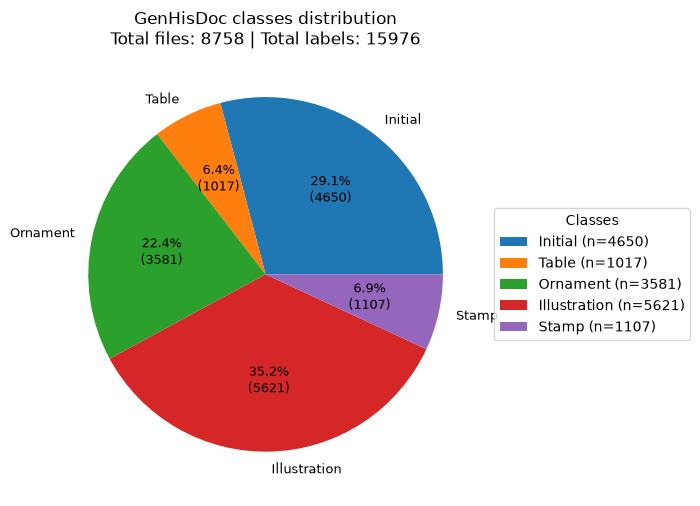
\includegraphics[scale=0.9]{img/distribution.png}
\end{figure}

\section{Description des modèles entraînés}

 Le dépôt \href{https://huggingface.co/Anarchiviste/GenHisDoc_model}{Huggin Face} contient deux modèles entraînés durant le stage (GenHisDoc YOLOV26 et YOLOV8) ainsi que les modèles YOLOV5 déployés sur AIKON. On y trouve un script pour faire tourner des inférences, un script pour générer des métriques suite à l'inférence et un script pour filtrer uniquement les illustrations (pour pouvoir comparer à AIKON qui est monoclasse)

\subsection{GenHisDoc YOLOv26L}

Algorithme : YOLOv26 Large 

Nombre d'époques : 100 

Taille du batch : 8 

Taille images: 640x640

\begin{figure}[H]
	\centering
	\begin{subfigure}{0.48\textwidth}
		\centering
		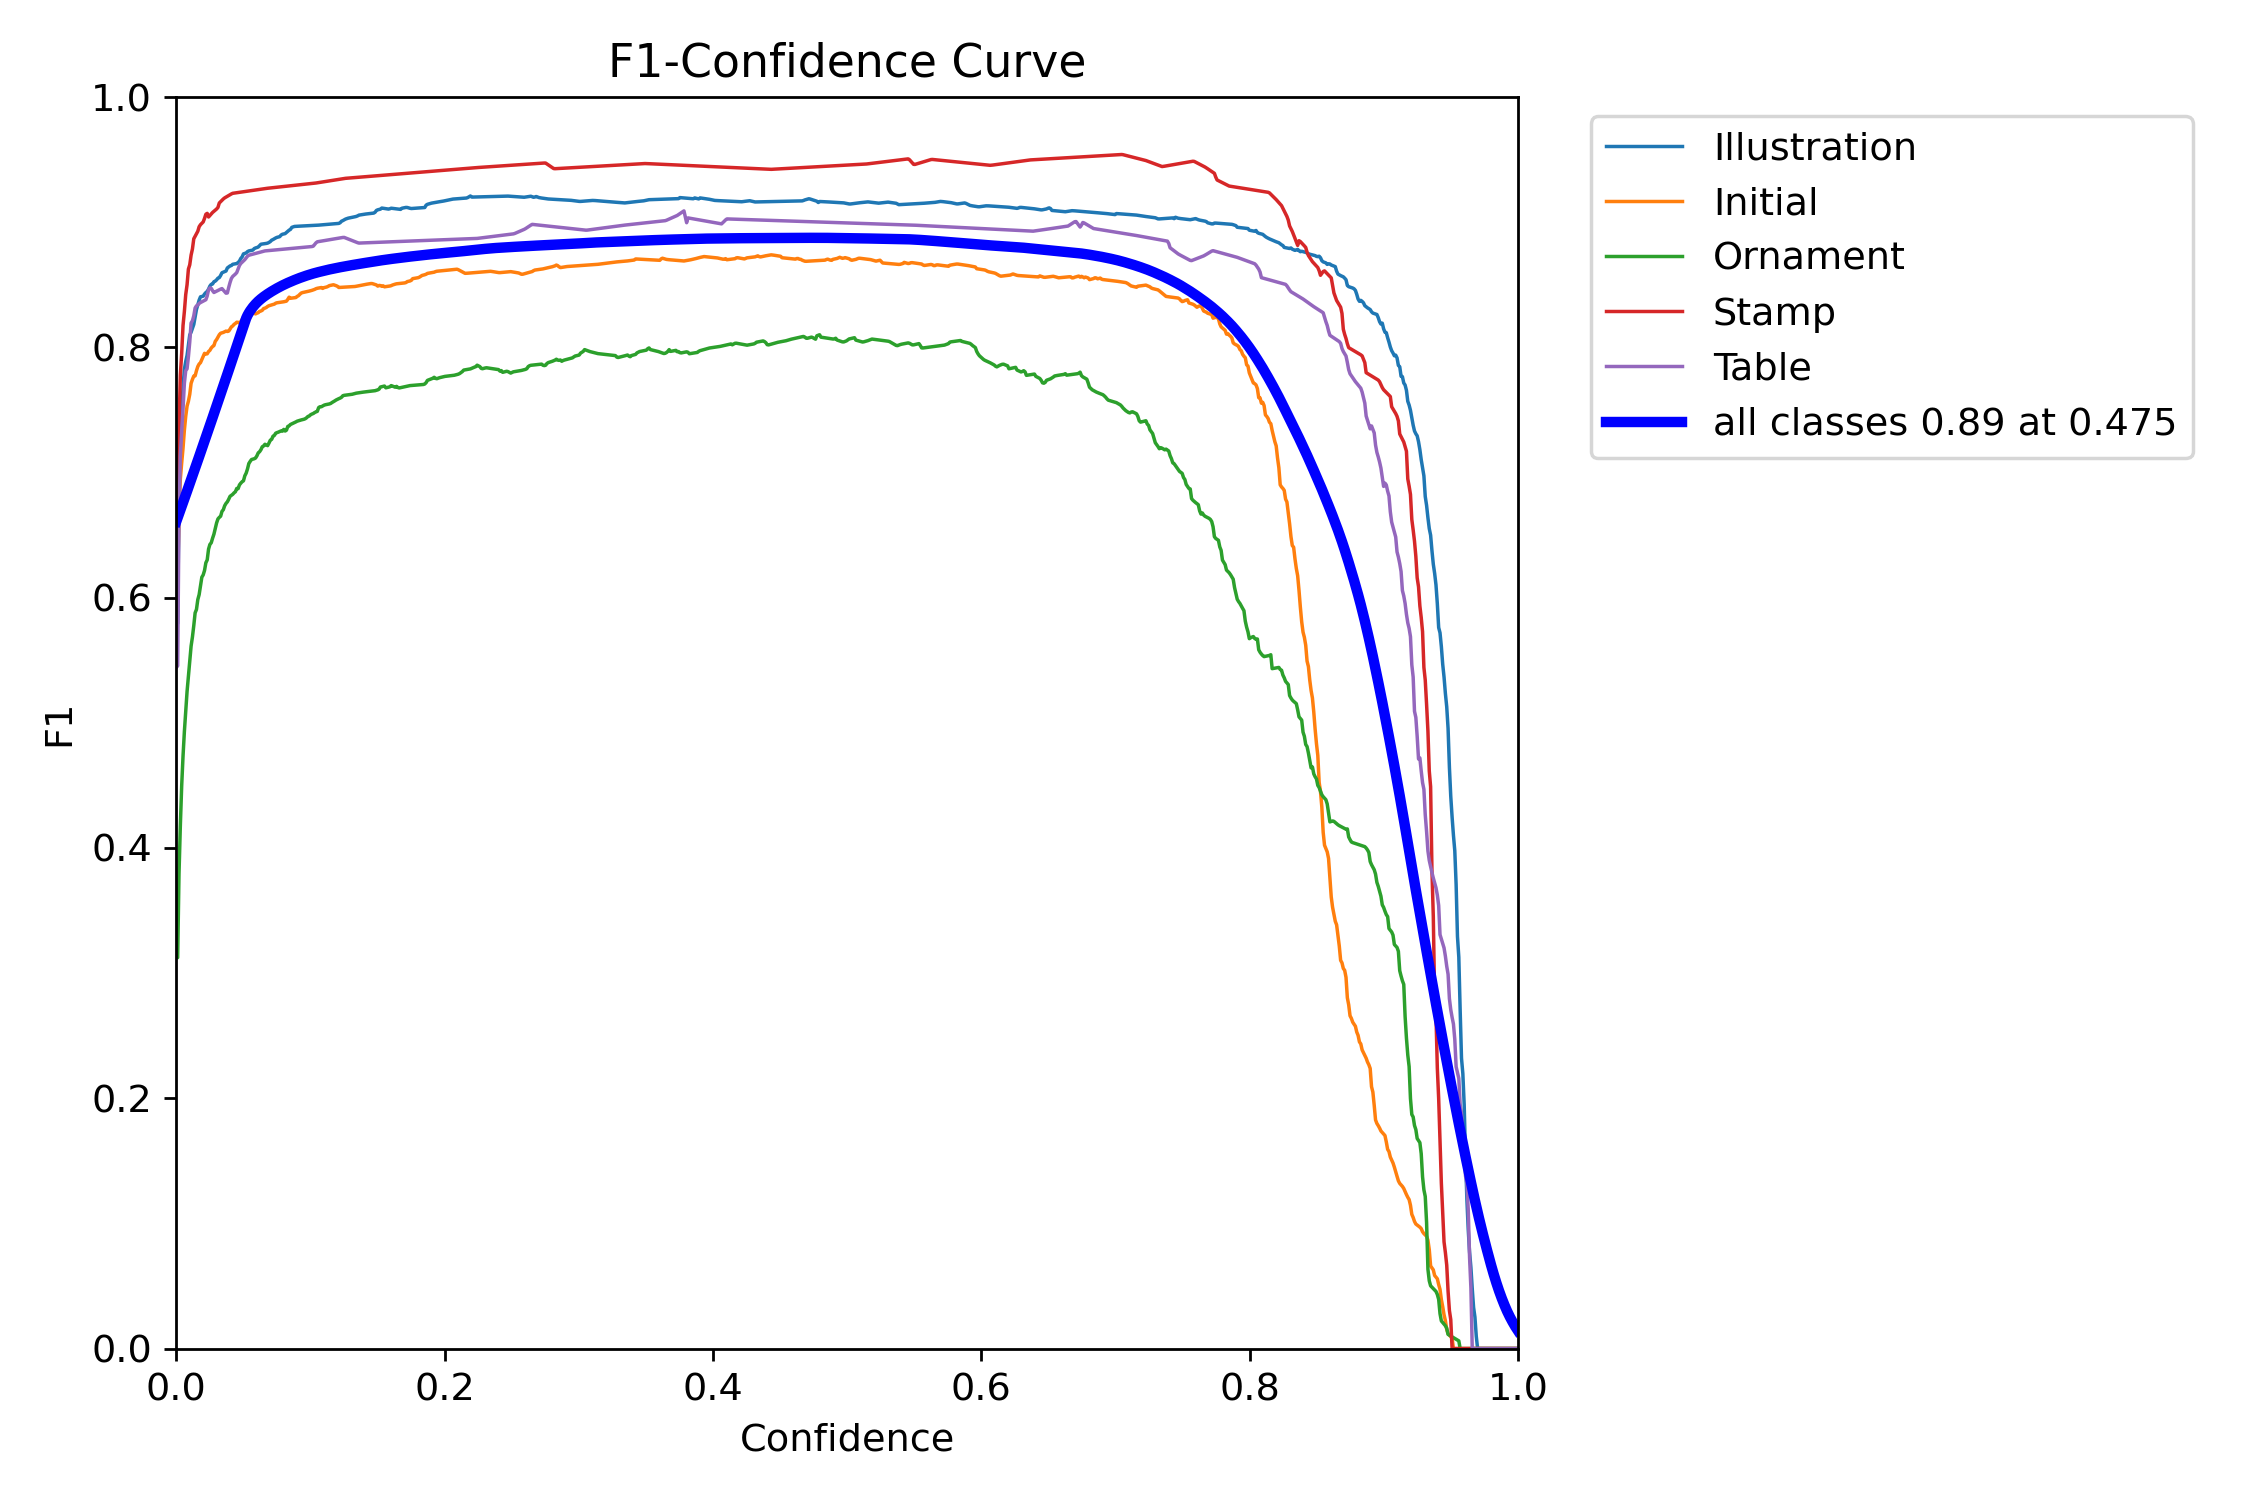
\includegraphics[width=\linewidth, height=8cm, keepaspectratio]{img/BoxF1_curve.png}
		\caption{Score F1}
	\end{subfigure}
	\hfill
	\begin{subfigure}{0.48\textwidth}
		\centering
		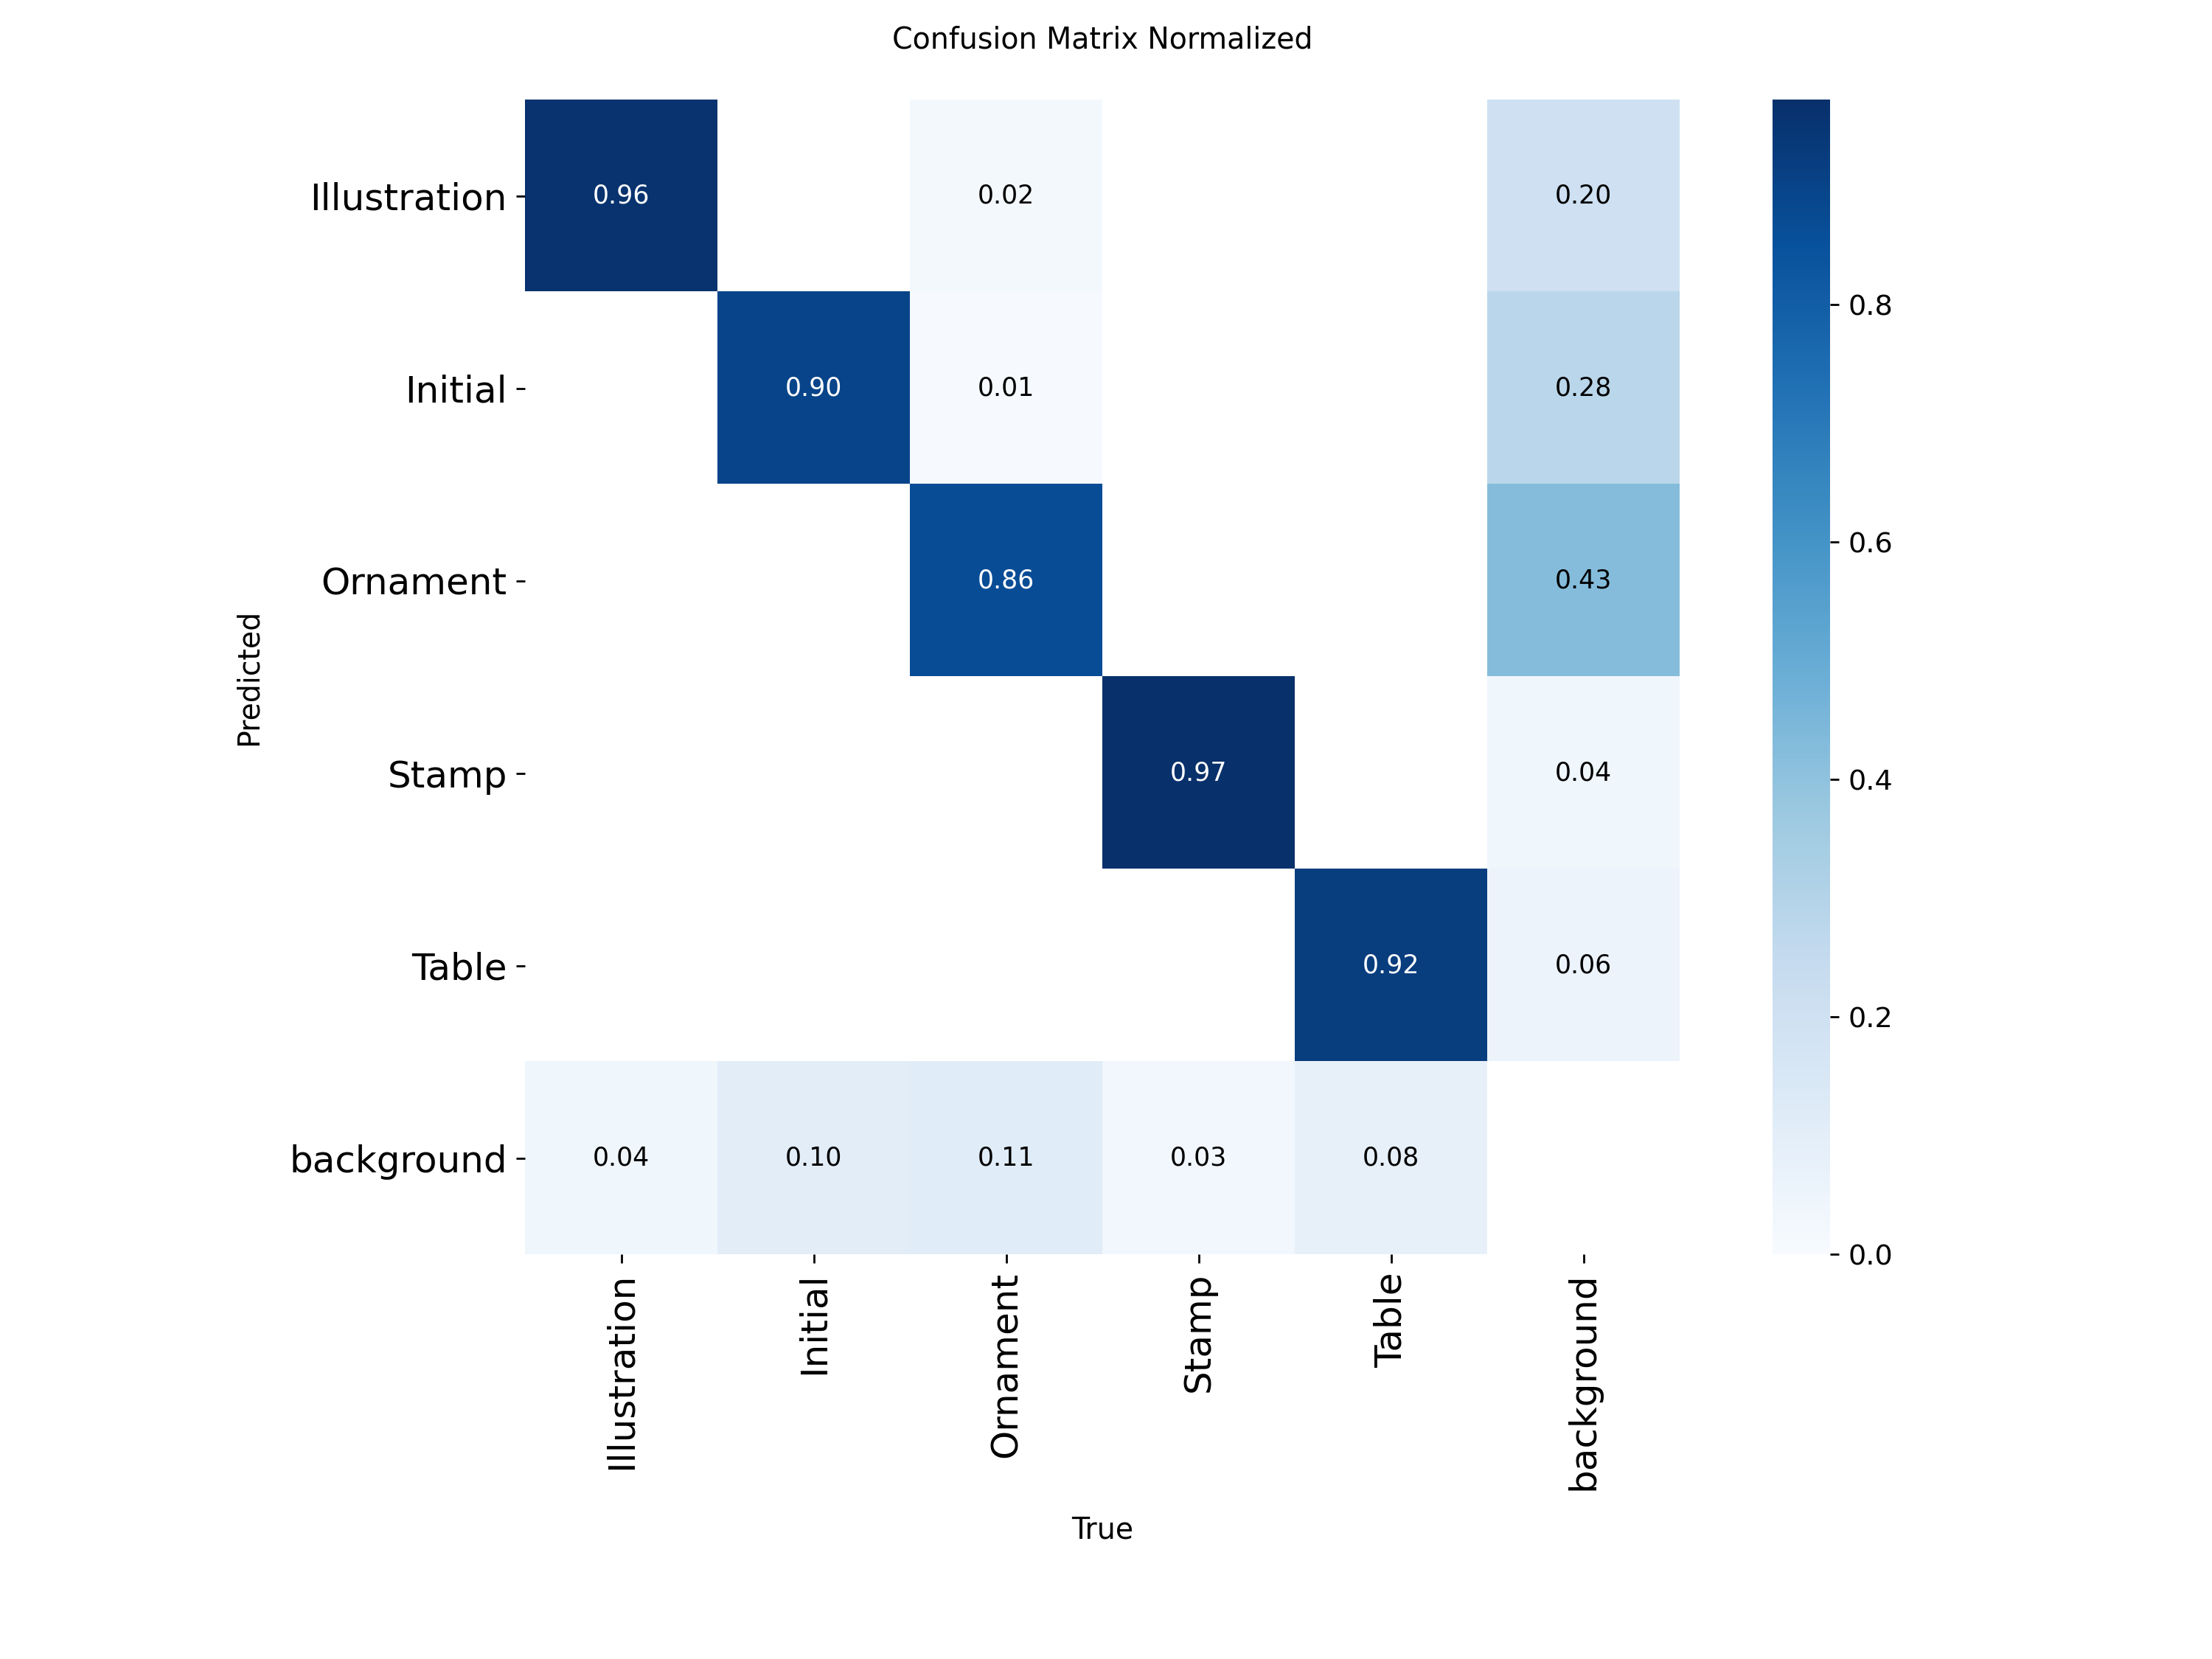
\includegraphics[width=\linewidth, height=8cm, keepaspectratio]{img/confusion_matrix_normalized.png}
		\caption{Matrice de confusion normalisée}
	\end{subfigure}
	\caption{Représentation des scores F1 et de la matrice de confusion normalisée des classes du YOLOV26 Large entrainé sur GenHisDoc.}
\end{figure}

\subsection{GenHisDoc YOLOV8L}

Algorithme : YOLOv8 Large 

Nombre d'époques : 100 

Taille du batch : 8 

Taille images: 640x640

\begin{figure}[H]
	\centering
	\begin{subfigure}{0.48\textwidth}
		\centering
		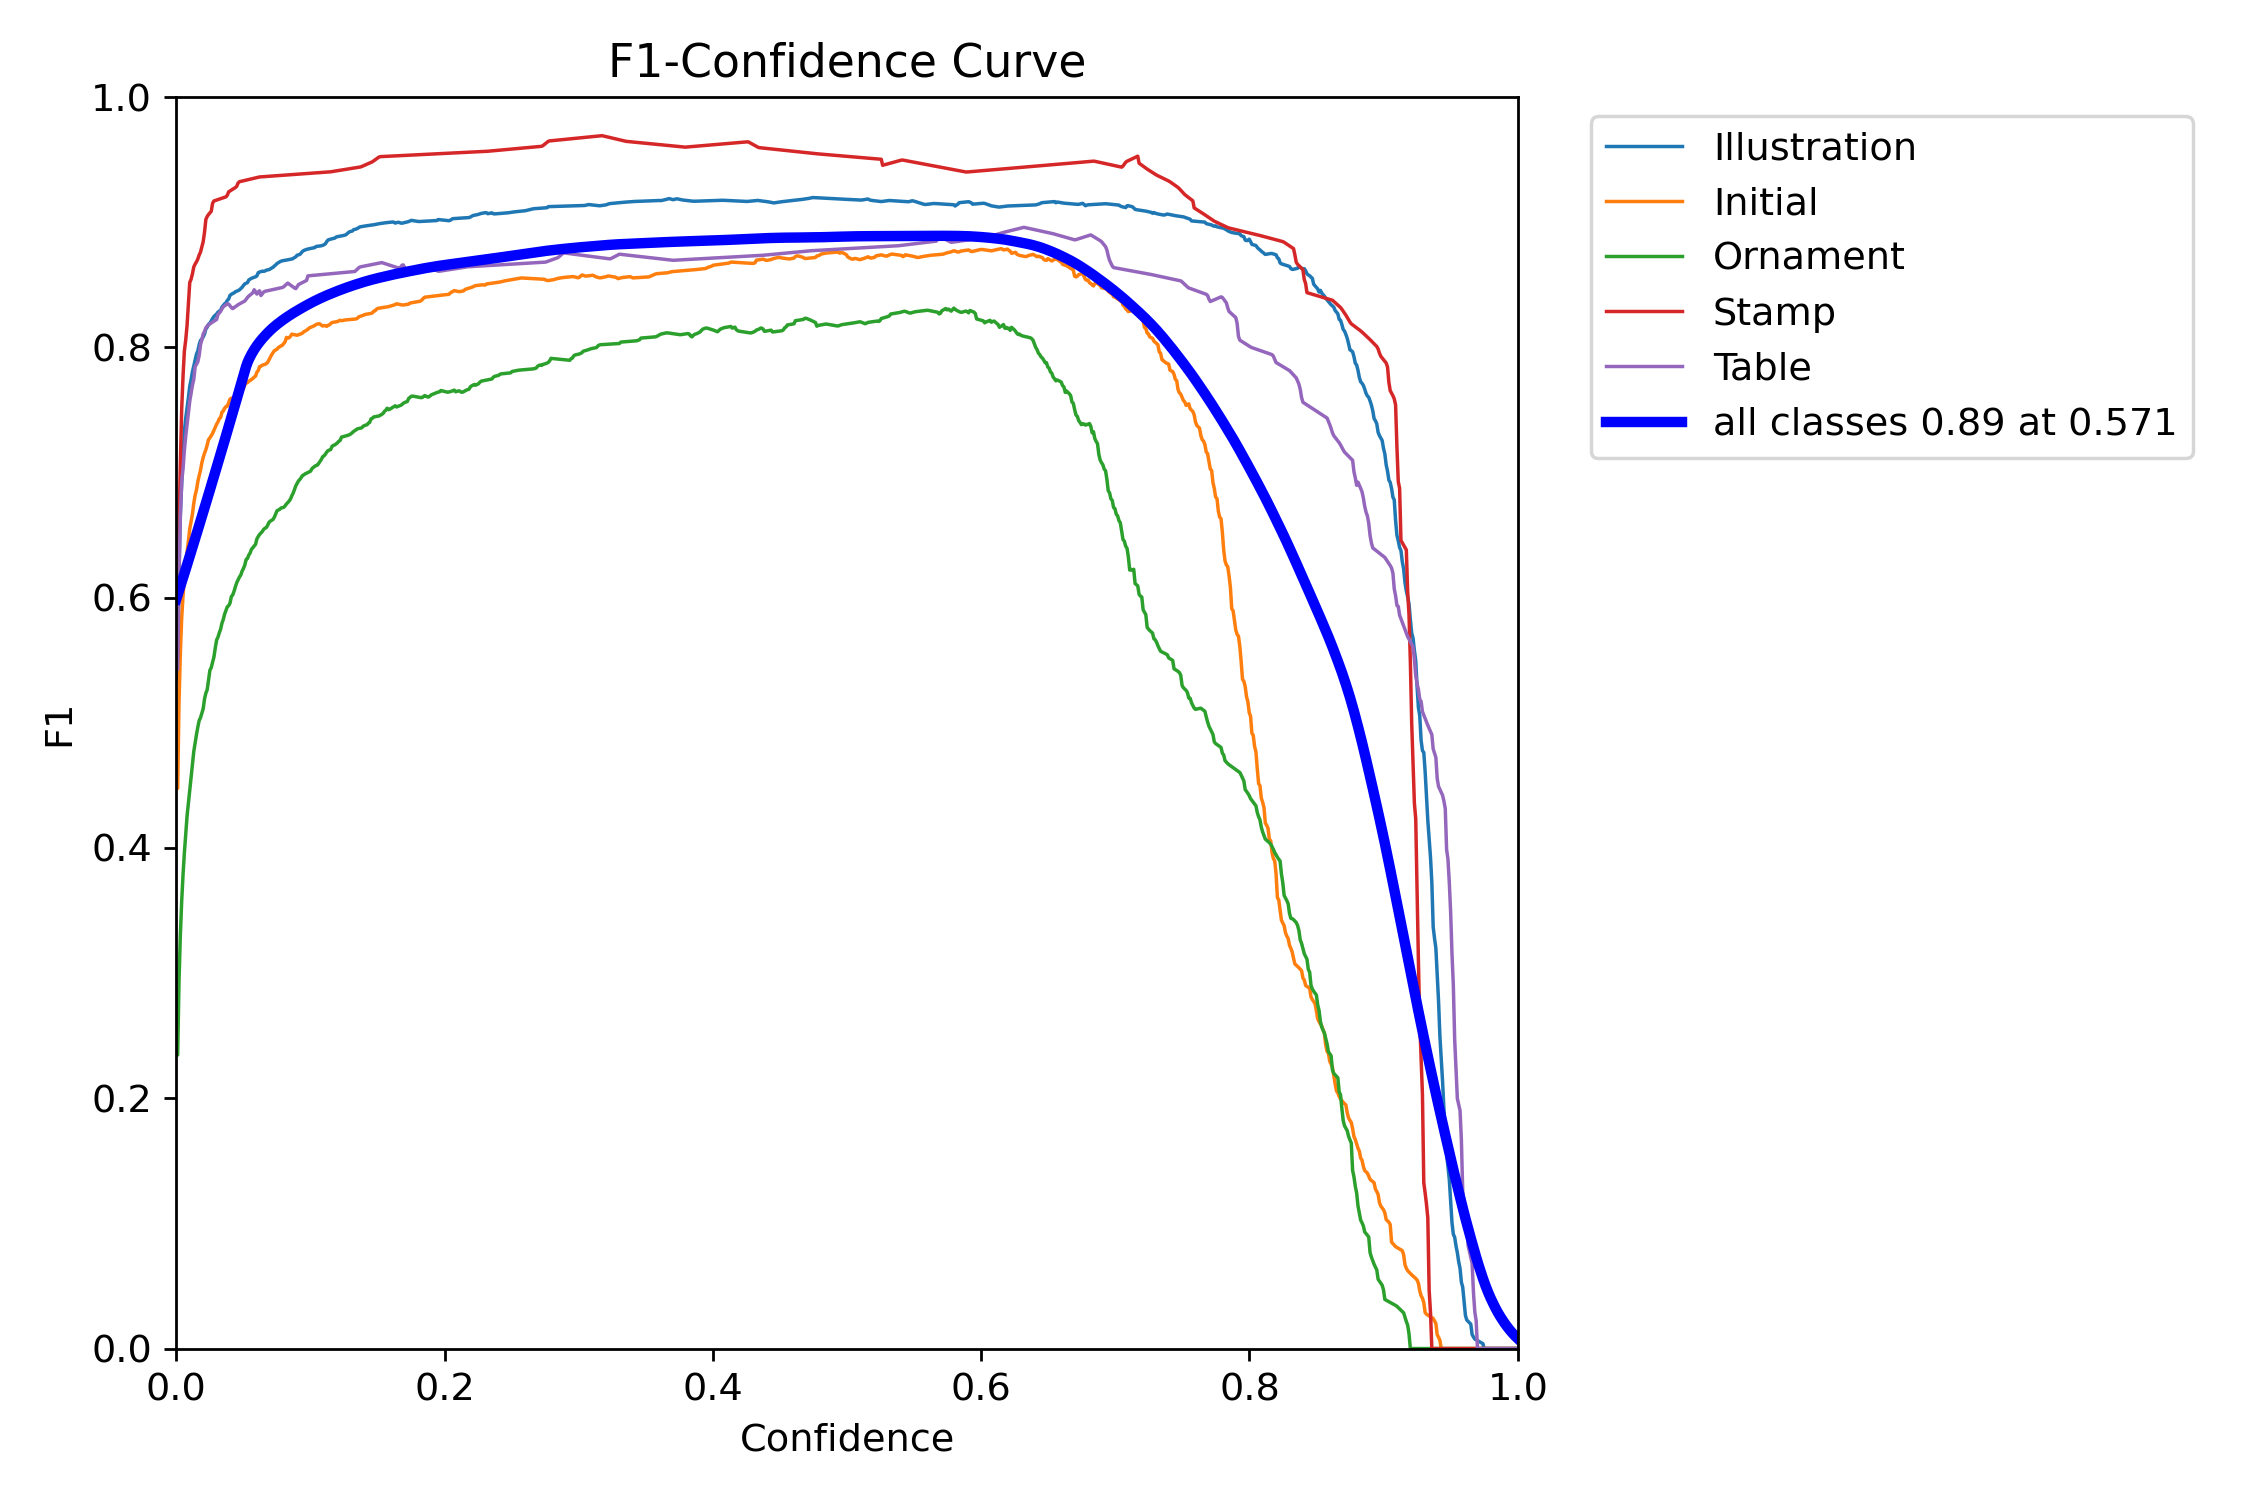
\includegraphics[width=\linewidth, height=8cm, keepaspectratio]{img/F1V8.png}
		\caption{Score F1}
	\end{subfigure}
	\hfill
	\begin{subfigure}{0.48\textwidth}
		\centering
		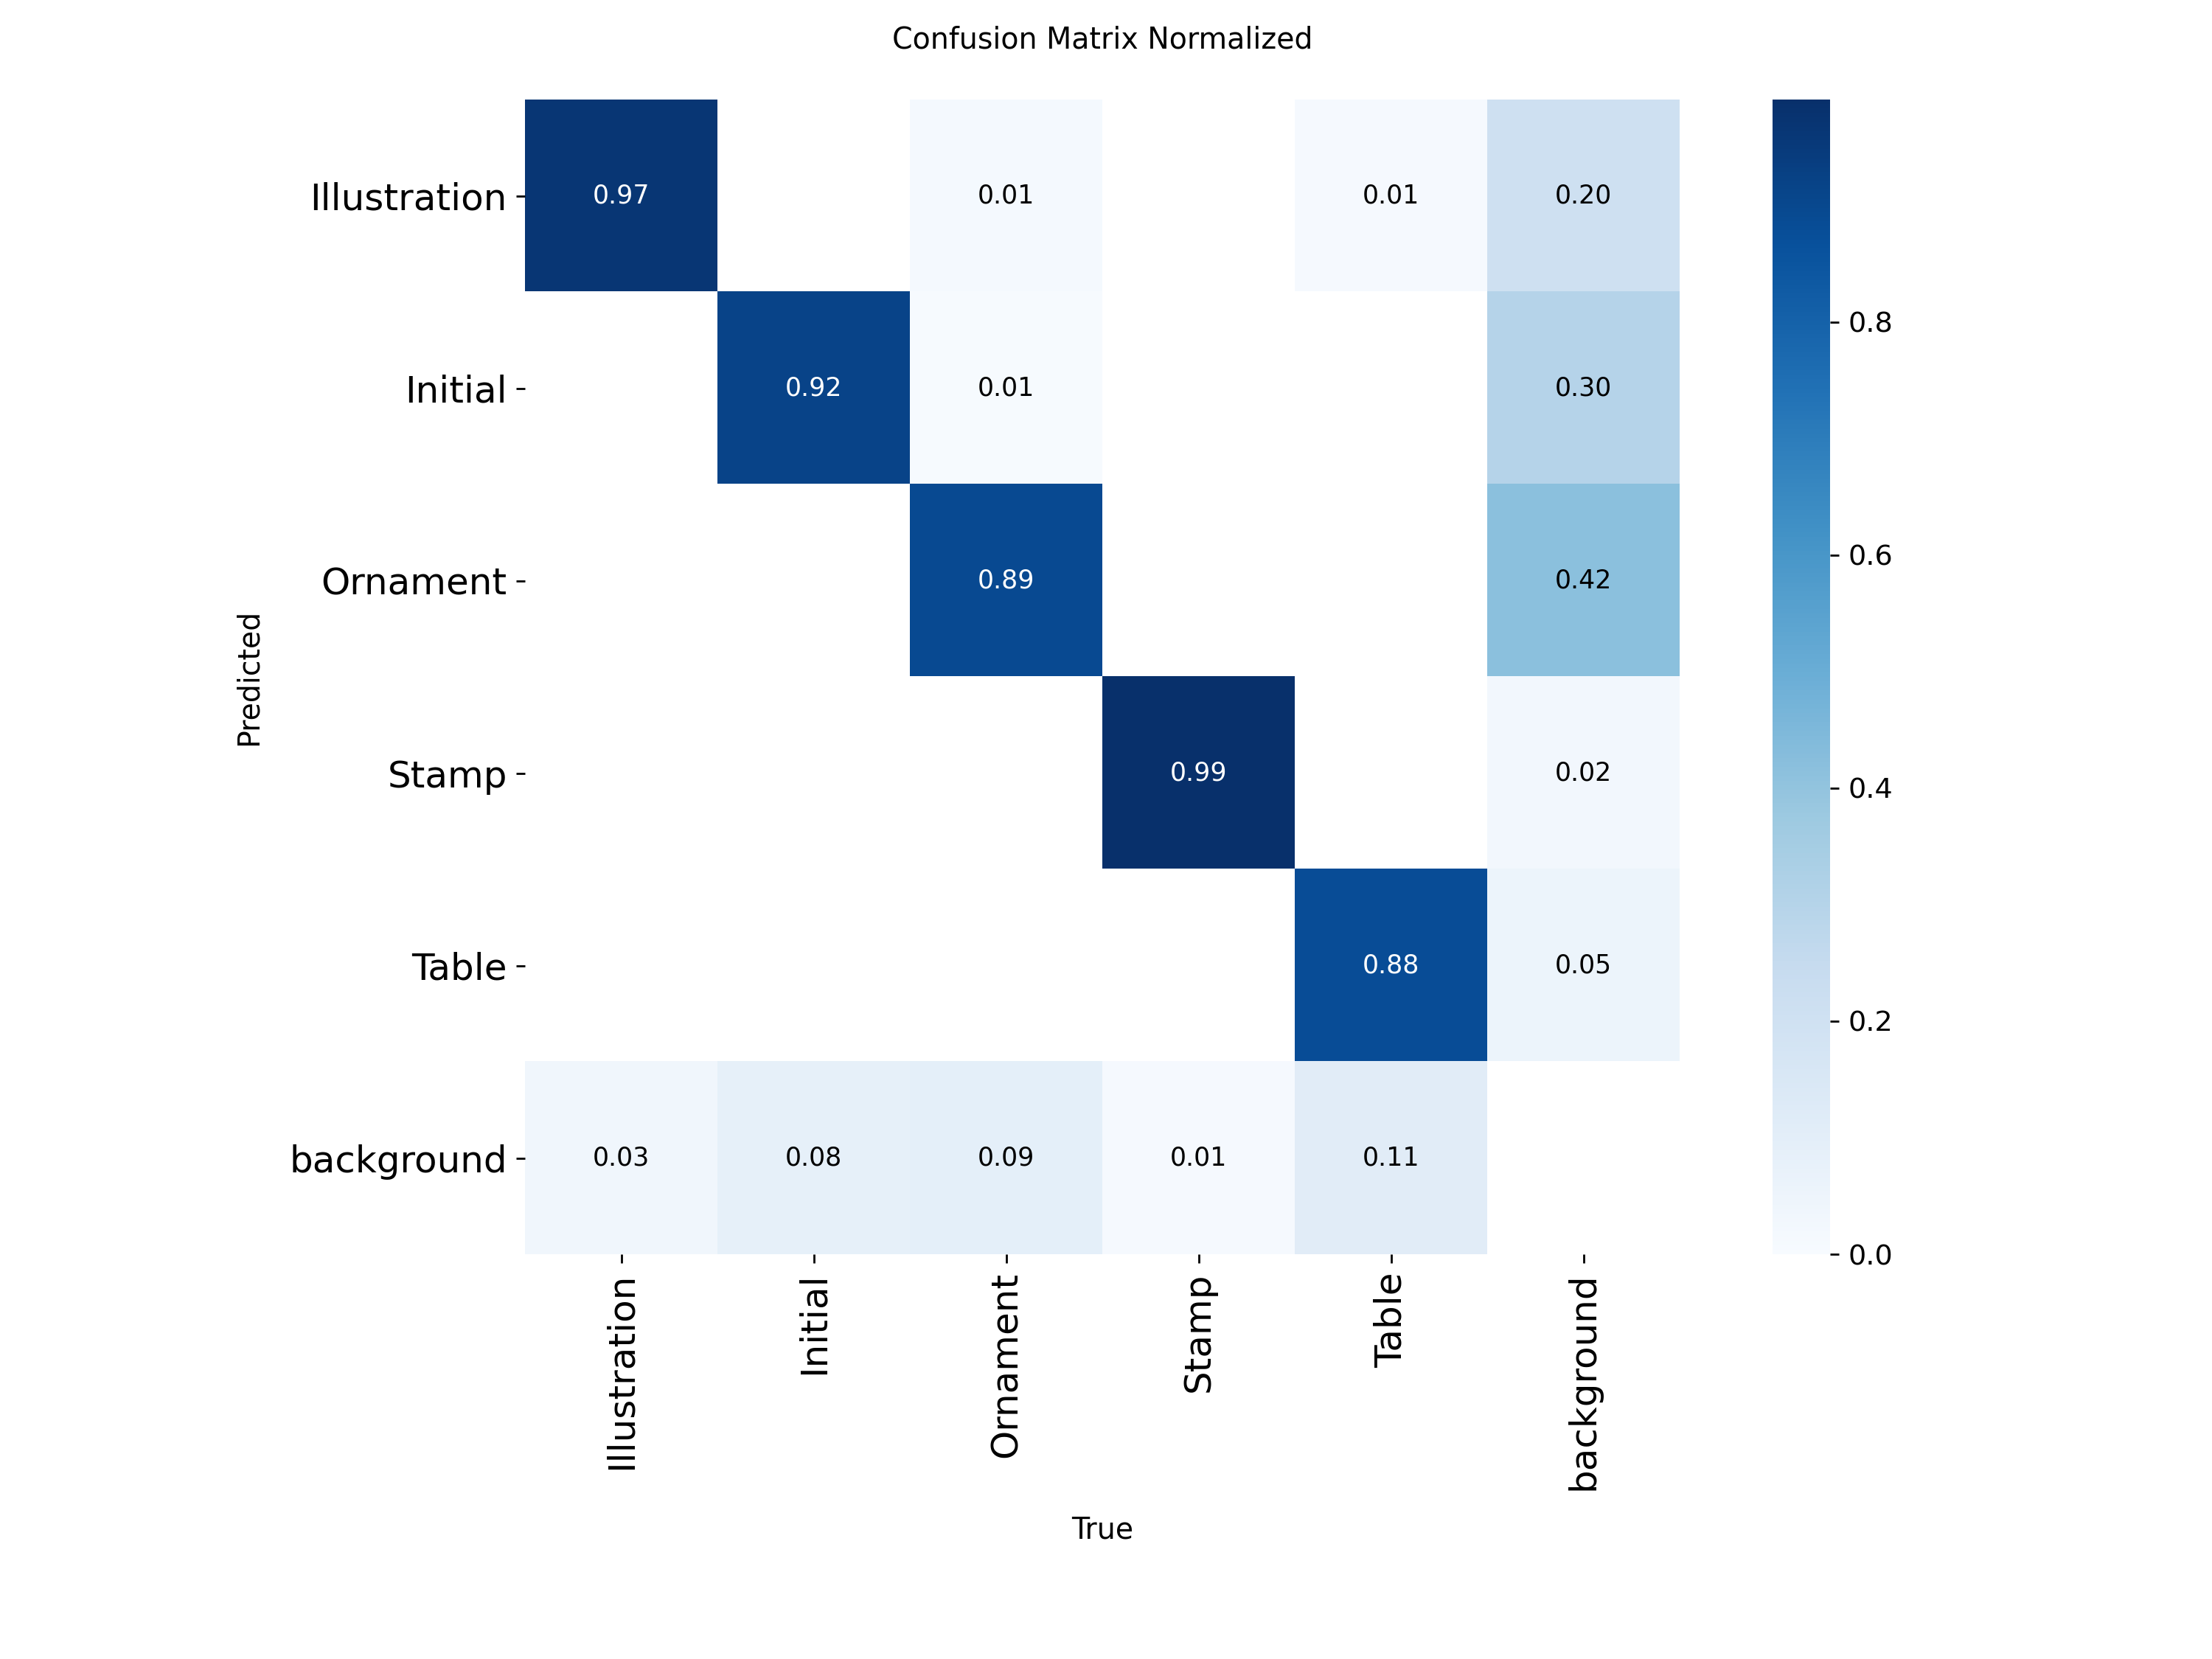
\includegraphics[width=\linewidth, height=8cm, keepaspectratio]{img/CONFUSIONV8.png}
		\caption{Matrice de confusion normalisée}
	\end{subfigure}
	\caption{Représentation des scores F1 et de la matrice de confusion normalisée des classes du YOLOV8 Large entrainé sur GenHisDoc.}
\end{figure}

\subsection[Benchmark Aikon]{Benchmark du YOLOV5 \og Illustation \fg{} d'AIKON sur GenHisDoc Test}

\begin{table}[H]
	\centering
	\ra{1.25}
	\caption{Comparaison des résultats d'évaluation entre GenHisDoc YOLOV26 Large et Aikon YOLOV5 Large}
	\begin{tabular}{lccc}
		\toprule
		& \multicolumn{2}{c}{\textbf{GenHisDoc}} & \textbf{Aikon} \\
		\cmidrule(r){2-3} \cmidrule(l){4-4}
		\textbf{Métrique / Indicateur} & \textbf{Illustration} & \textbf{Toutes classes} & \textbf{Illustration} \\
		\midrule
		\multicolumn{4}{l}{\textit{Données de test et Détection}} \\
		\hspace{1em} Fichiers traités & 876 & 876 & 876 \\
		\hspace{1em} Nombre total de GT & 558 & 1659 & 558 \\
		\hspace{1em} IoU Moyen (Détections) & 0,9033 & 0,8595 & 0,8762 \\
		\midrule
		\multicolumn{4}{l}{\textit{Performance globale}} \\
		\hspace{1em} AP@50 (mAP@50) & \textbf{0,8787 (87,87\%)} & 0,8404 (84,04\%) & 0,4815 (48,15\%) \\
		\midrule
		\multicolumn{4}{l}{\textit{Métriques au seuil fixe ($\ge$ 0,25)}} \\
		\hspace{1em} Vrais Positifs (TP) & 501 & 1448 & 355 \\
		\hspace{1em} Faux Positifs (FP) & 80 & 261 & 208 \\
		\hspace{1em} Faux Négatifs (FN) & 57 & 211 & 203 \\
		\hspace{1em} Précision & 0,8623 & 0,8473 & 0,6306 \\
		\hspace{1em} Rappel (Recall) & 0,8978 & 0,8728 & 0,6362 \\
		\hspace{1em} Score F1 & \textbf{0,8797} & 0,8599 & 0,6334 \\
		\bottomrule
	\end{tabular}
\end{table}

\section{Aikoncli}

Le dépot \href{https://github.com/Anarchiviste/aikoncli/tree/main}{GitHub} contient le code d'Aikon CLI. C'est un petit outil en ligne de commande conçu pour télécharger des images et des annotations de boîtes englobantes (bounding boxes) connectées à un serveur d'annotations IIIF Aikon. Le format de sortie suit le système d'annotation de style YOLO, s'organisant autour de deux répertoires distincts (images et labels) contenant des paires de fichiers associés (par exemple, 1.jpg et 1.txt).


 \chapter[Annexes : Formations]{Rendus Techniques : formation et documentation}
 
 Ce dépôt \href{https://github.com/Anarchiviste/GenHisDoc_Lab/edit/main/labelstudio_reannotation.md}{GitHub} contient un tutoriel que nous avons produits dans le cadre de la mise en place de l'environnement de réannotation Label Studio. Le stage s'étant déroulé entièrement en anglais, l'ensemble des travaux, des échanges et de la documentation technique a été produit dans cette langue. C'est pourquoi certains supports de rendu et documents présentés ici conservent leur terminologie originale anglaise.
 
 \label{chap:guideline}
 \chapter[Guidelines d'Annotations]{Rendus Techniques : guidelines d'annotations}

Loin d'être destiné à être utilisé tel quel par des annotateurs, ce guide d'annotation de GenHisDoc a pour principal objectif de consigner la méthodologie employée pour produire les annotations et les corrections du jeu de données. Le stage s'étant déroulé entièrement en anglais, l'ensemble des travaux, des échanges et de la documentation technique a été produit dans cette langue. C'est pourquoi certains supports de rendu et documents présentés ici conservent leur terminologie originale en anglais.

\hrulefill

\section{Introduction}

Welcome to this data labelling guide for historical corpora annotation. This document will provide you with all the information and context necessary for your work as an annotator. This document is available to you throughout your assignment and you should refer to it if you have any questions.

We want to produce annotations to train a model to detect different types of content in historical documents. To train the model, the annotations must be as consistent as possible.

\subsection{Context}

Our goal is to create an automated system for extracting visual elements using machine learning technology. For this, we have high-quality data, annotated and manually corrected by human hands.

We are currently working on a study of the dissemination of texts by studying images. In this project, we need only interested in the visual elements and we will completely disregard text.

The page of a historical document is composed of text, illustrations, ornaments and other elements added after the creation of the object, such as glosses, comments, stamps, drawings, traces of wear.

\subsection{Task Definition}

You are an annotator and your goal is to annotate the visual elements of the page. To do this, you will draw straight rectangles around the elements that have a label. The 5 labelling tags are the following : 

\begin{itemize}
    \item 0: "Illustration"
    \item 1: "Ornament"
    \item 2: "Initial"
    \item 3: "Stamp"
    \item 4: "Table"
\end{itemize}


\hrulefill
\section{General rules}


Here are some general rules of good practice for your work.

\subsection{Hug the border of the object as tightly as possible}

A precise annotation like the one shown in the image~\ref{fig:goodfit} captures the entire visual element and is as close as possible to the boundaries to reduce confusion for the machine learning model.

\begin{figure}
    \centering
    \begin{subfigure}{0.48\textwidth}
        \centering
        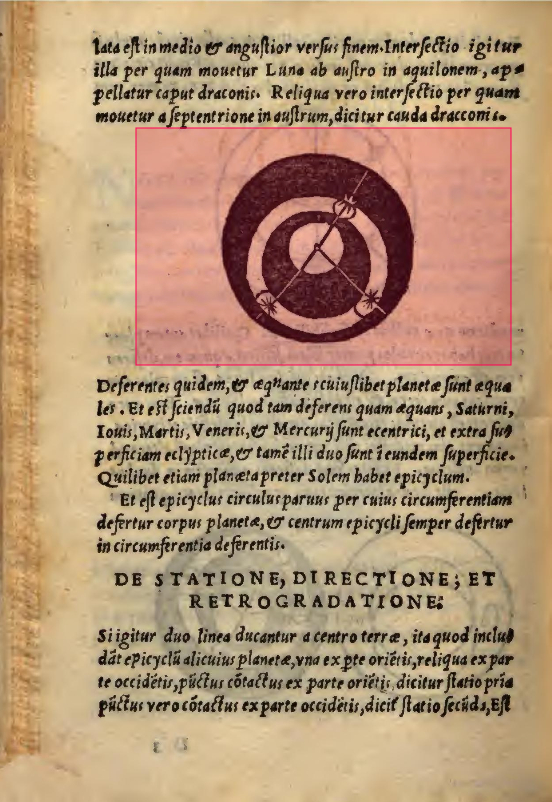
\includegraphics[width=\linewidth, height=7cm, keepaspectratio]{Guidelines/bad_fitting.png}
        \caption{ {\color{red}\faClose} Here, the annotation is too large.}
        \label{fig:badfit}
    \end{subfigure}
    \hfill
    \begin{subfigure}{0.48\textwidth}
        \centering
        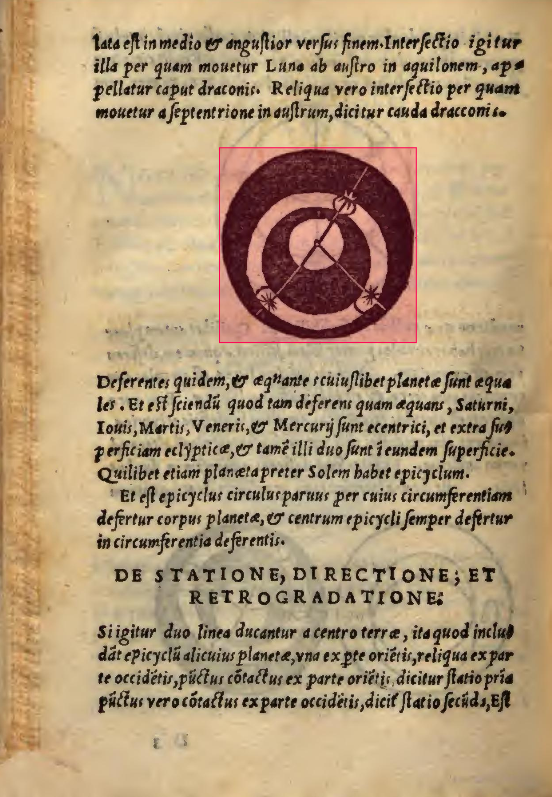
\includegraphics[width=\linewidth, height=7cm, keepaspectratio]{Guidelines/good_fitting.png}
        \caption{ {\color{green}\faCheck} Here is the correct way to annotate an element: the borders are closed to the end of the element without cutting them.}
        \label{fig:goodfit}
    \end{subfigure}
    \caption{Hug the border of the object as tightly as possible.}
\end{figure}

\subsection{Separate the elements that are not visually connected.}

Each distinct visual element must receive its own annotation (bounding box), even if several elements appear to form a coherent whole from the point of view of meaning or composition intended by the author of the document as seen in Figure~\ref{fig:unification} and Figure~\ref{fig:separation}.

Two elements can be "linked" in the author's intention (for example, a human figure and a dog figure accompanying it, or related but non-touching ornamentation) without being visually connected (that is, without sharing a common background, frame, or direct contact). In this case, the annotations are separate.

If several elements share the same background or frame (for example, several symbols or drawings printed on a single continuous graphic strip), they can be grouped into a single annotation, because they are physically or visually unified on the medium as seen in Figure~\ref{fig:example_illustration_frame} and \ref{fig:example_illustration_frame_rule} .

\begin{figure}
    \centering
    \begin{subfigure}{0.48\textwidth}
        \centering
        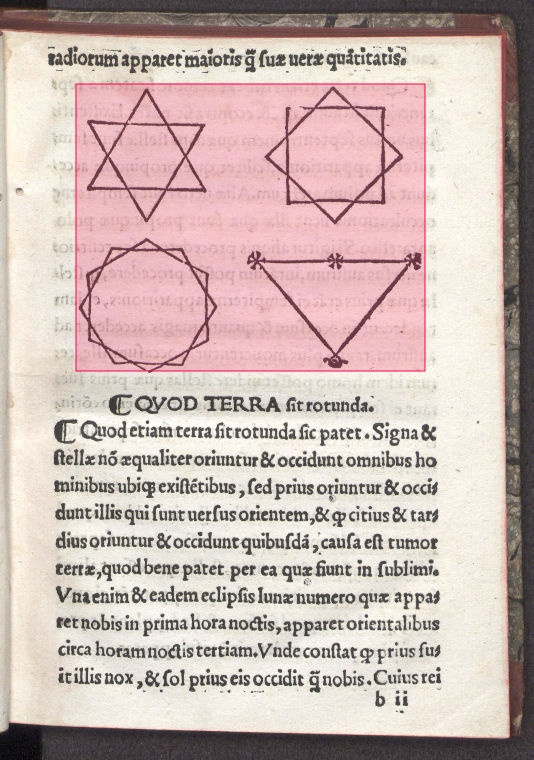
\includegraphics[width=\linewidth, height=7cm, keepaspectratio]{Guidelines/unification.png}
        \caption{{\color{red}\faClose} These elements, although clearly grouped together by the author, should not be annotated in this way.}
        \label{fig:unification}
    \end{subfigure}
    \hfill
    \begin{subfigure}{0.48\textwidth}
        \centering
        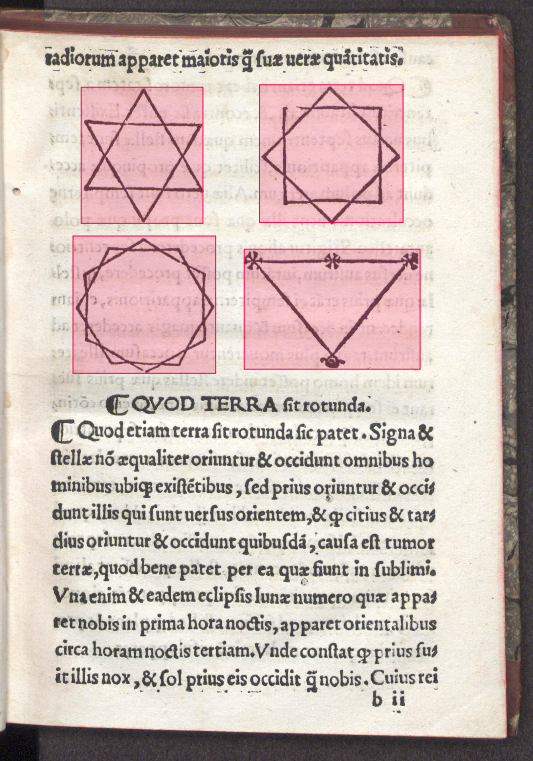
\includegraphics[width=\linewidth, height=7cm, keepaspectratio]{Guidelines/separation.png}
        \caption{{\color{green}\faCheck} Here's how we want to annotate several elements.}
        \label{fig:separation}
    \end{subfigure}
    \caption{Separate element that are not visualy linked}
\end{figure}

\subsection{Avoid item overlap} 

\textbf{This is not a strict rule}. In many documents, elements overlap and are interconnected, as illustrated in Figure \ref{fig:good_overlap}. The section on class definitions and examples will show you the cases where overlapping annotations are necessary and those where they can be avoided.

\begin{figure}
    \centering
    \begin{subfigure}{0.48\textwidth}
        \centering
        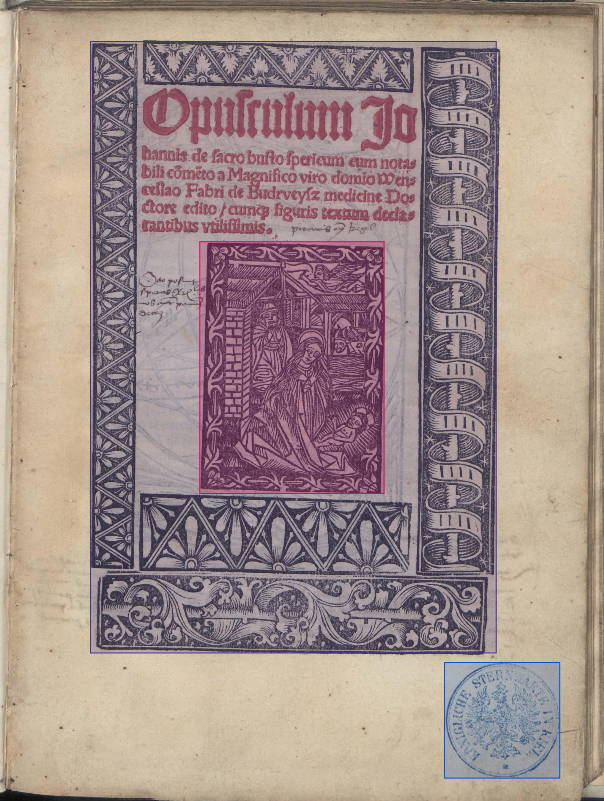
\includegraphics[width=\linewidth, height=7cm, keepaspectratio]{Guidelines/overlap.png}
        \caption{{\color{red}\faClose} The annotation of the ornament overlap against to much elements}
        \label{fig:bad_overlap}
    \end{subfigure}
    \hfill
    \begin{subfigure}{0.48\textwidth}
        \centering
        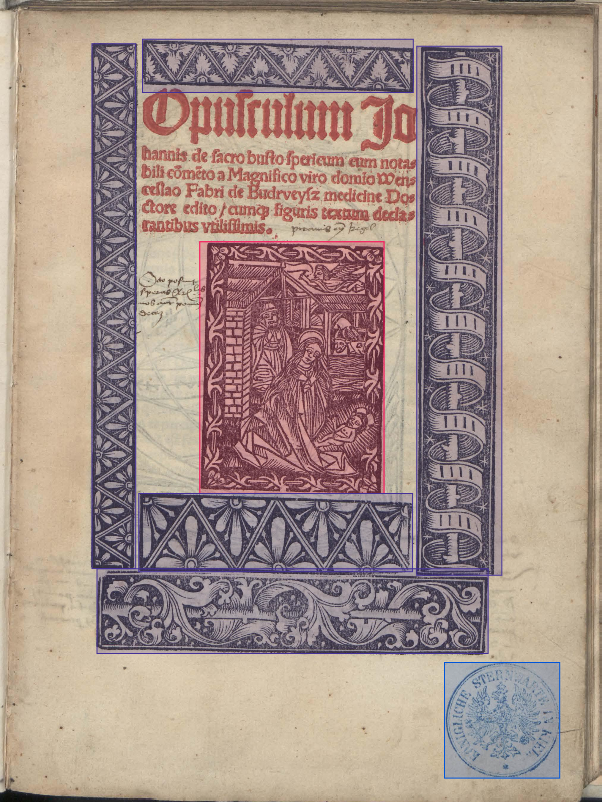
\includegraphics[width=\linewidth, height=7cm, keepaspectratio]{Guidelines/correct_overlap.png}
        \caption{{\color{green}\faCheck} We decided to cut out the decorative elements to avoid overlapping.}
        \label{fig:good_overlap}
    \end{subfigure}
    \caption{Avoid item overlap between classes}
\end{figure}

\subsection{Annotate only the main page}

Do not annotate anything that is not on the main page. As shown in example \ref{fig:main_page}, if the scan was done for two pages, annotate it as shown in \ref{fig:both_page}.

\begin{figure}
    \centering
    \begin{subfigure}{0.48\textwidth}
        \centering
        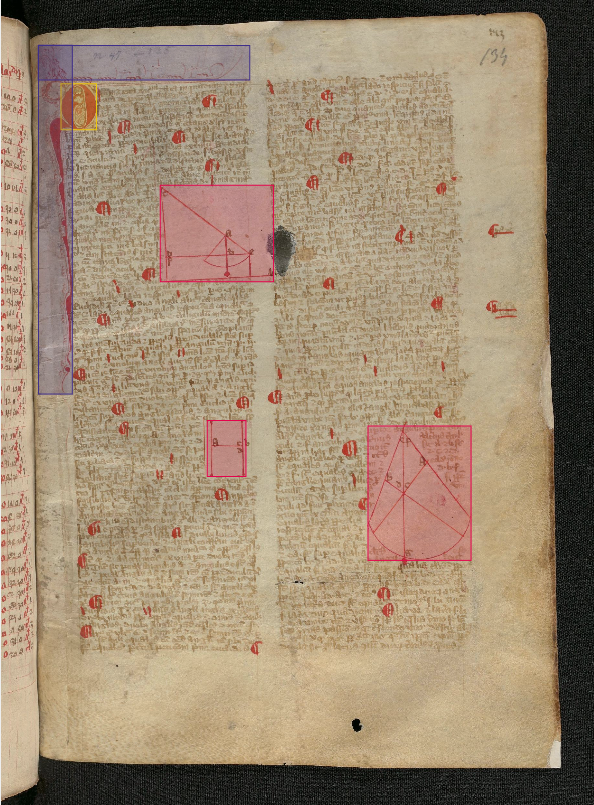
\includegraphics[width=\linewidth, height=7cm, keepaspectratio]{Guidelines/Screenshot_20260702_112821.png}
        \caption{Do not annotate the tables on the little bit of the other page.}
        \label{fig:main_page}
    \end{subfigure}
    \hfill
    \begin{subfigure}{0.48\textwidth}
        \centering
        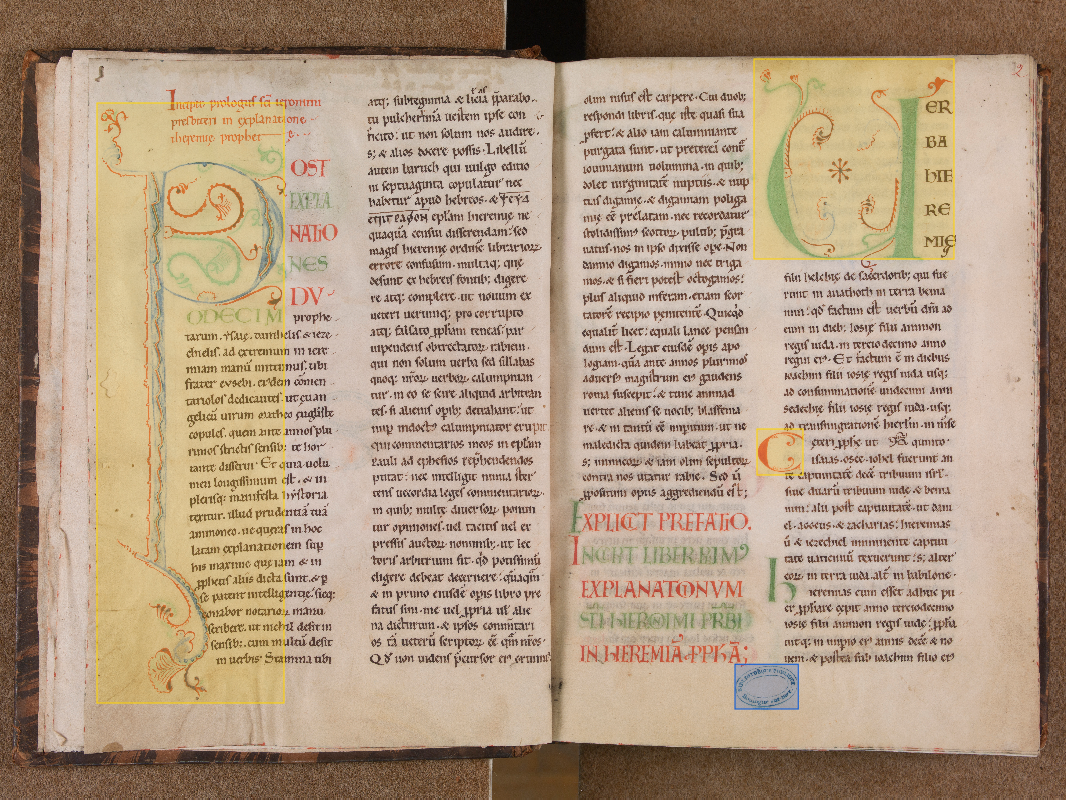
\includegraphics[width=\linewidth, height=7cm, keepaspectratio]{Guidelines/Screenshot_20260702_135302_2.png}
        \caption{If the scan is done for two pages, then you must annotate the elements of both pages.}
        \label{fig:both_page}
    \end{subfigure}
    \caption{Annotate only the main page}
\end{figure}

\subsection{Annotate what is visible, not what you infer}

Label only the content that is actually present and legible in the document, as shown in the image \ref{fig:completion}. Do not extend a bounding box or complete an area based on what you assume to be there (for example, a torn page, an erased stamp, text hidden by a fold).

\begin{figure}
    \centering
    \begin{subfigure}{0.48\textwidth}
        \centering
        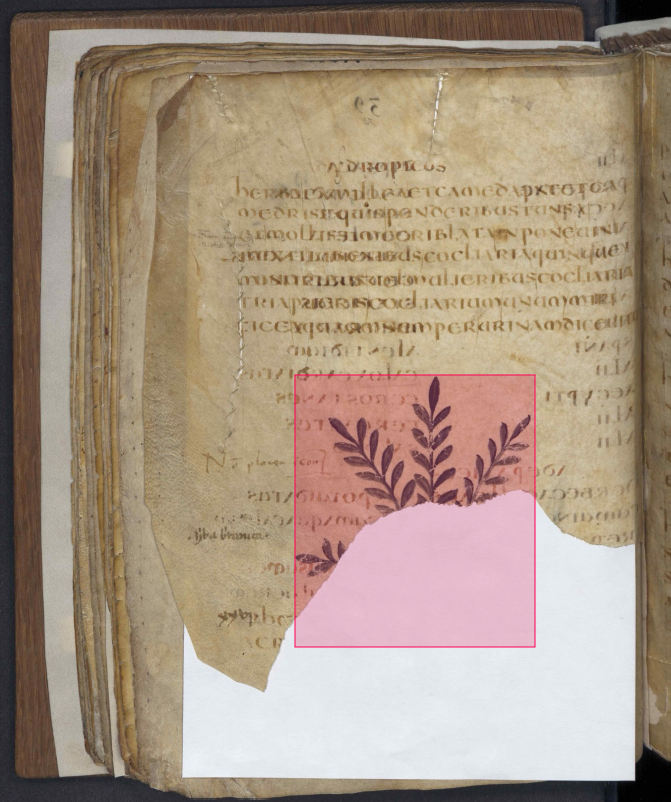
\includegraphics[width=\linewidth, height=7cm, keepaspectratio]{Guidelines/tomuch.png}
        \caption{{\color{red}\faClose} This annotation attempts to complete an element that is no longer visible.}
        \label{fig:completion}
    \end{subfigure}
    \hfill
    \begin{subfigure}{0.48\textwidth}
        \centering
        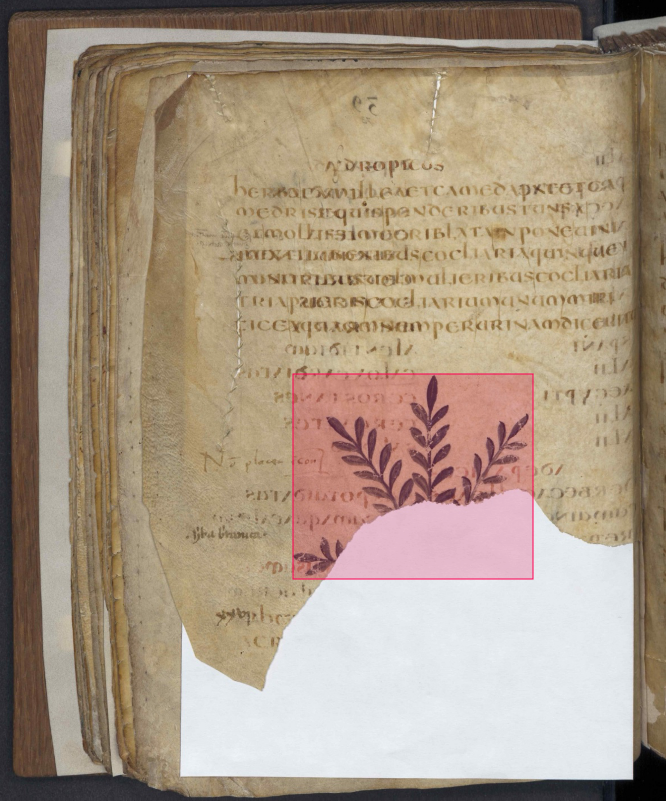
\includegraphics[width=\linewidth, height=7cm, keepaspectratio]{Guidelines/correct_amount.png}
        \caption{{\color{green}\faCheck} This annotation respects the limits of what is visible in the document.}
        \label{fig:fitting}
    \end{subfigure}
    \caption{Annotate what is visible, not what you infer}
\end{figure}

\subsection{Review your work before submitting.}

The annotation task can be arduous and tedious; it is advisable to check the quality of the annotations before moving on to the next image and to take regular breaks to stay alert and focused.

\hrulefill
\section{Class definition}

\begin{comment}

\begin{figure}
    \centering
    \begin{subfigure}{0.48\textwidth}
        \centering
        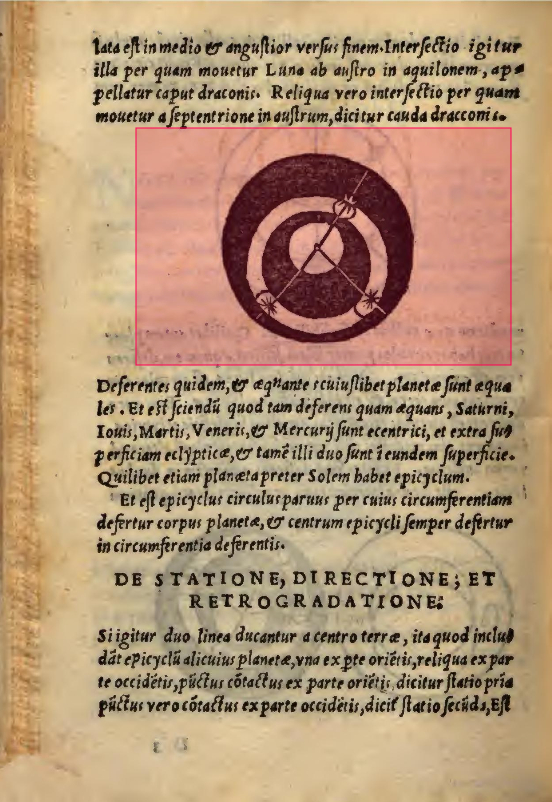
\includegraphics[width=\linewidth, height=7cm, keepaspectratio]{Guidelines/bad_fitting.png}
        \caption{ {\color{red}\faClose} The annotation is too large here.}
        \label{fig:badfit}
    \end{subfigure}
    \hfill
    \begin{subfigure}{0.48\textwidth}
        \centering
        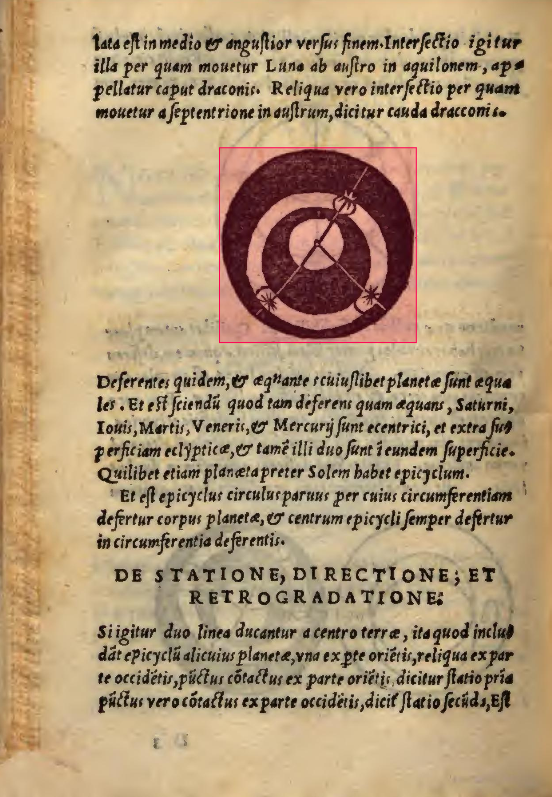
\includegraphics[width=\linewidth, height=7cm, keepaspectratio]{Guidelines/good_fitting.png}
        \caption{ {\color{green}\faCheck} This is the correct way of annotating an element, the borders are close to the end of the element without biting them.}
        \label{fig:goodfit}
    \end{subfigure}

\end{figure}

\end{comment}

You will be annotating the corpus of documents with 5 classes to describe elements inside historical documents:

\subsection{Illustration}

\subsubsection{Description}

The class "illustration" should be understood as a generic class encompassing all graphic elements. An illustration can be functional or artistic; its function is then to inform, illustrate, or entertain the reader.

Examples of illustrations within an image include paintings, photographs, drawings, mathematical graphs, charts, diagrams, symbols, and maps. What distinguishes an illustration from an ornament is its own semantics: it has a meaning that is interpreted in relation to the text, unlike an ornament which is purely decorative.

\begin{figure}
  \centering
  \begin{subfigure}{0.48\textwidth}
    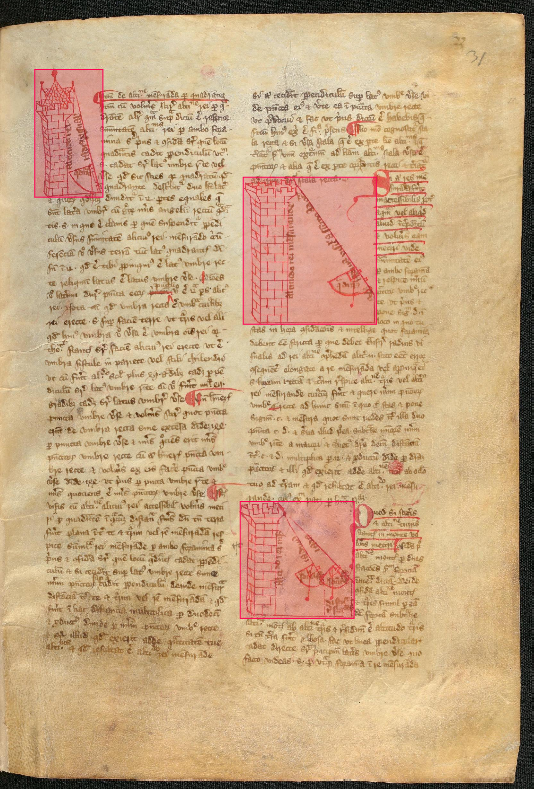
\includegraphics[width=\linewidth, height=7cm, keepaspectratio]{Guidelines/illustraiton_4.png}
    \caption{A geometry manuscript that illustrates angle calculations.}
  \end{subfigure}
  \hfill
  \begin{subfigure}{0.48\textwidth}
    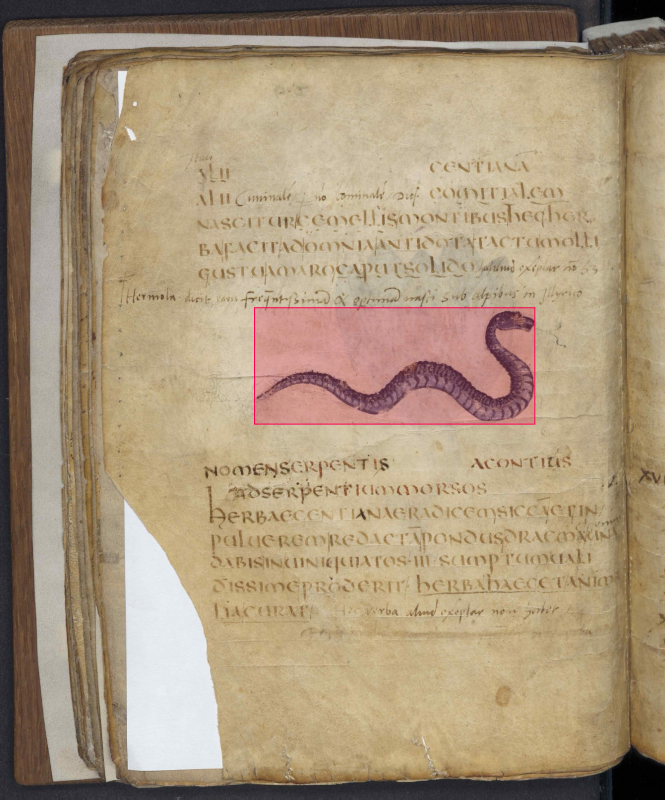
\includegraphics[width=\linewidth, height=7cm, keepaspectratio]{Guidelines/illustration_2.png}
    \caption{A handwritten bestiary with an illustration of a snake.}
  \end{subfigure}
  \hfill
  \begin{subfigure}{0.48\textwidth}
    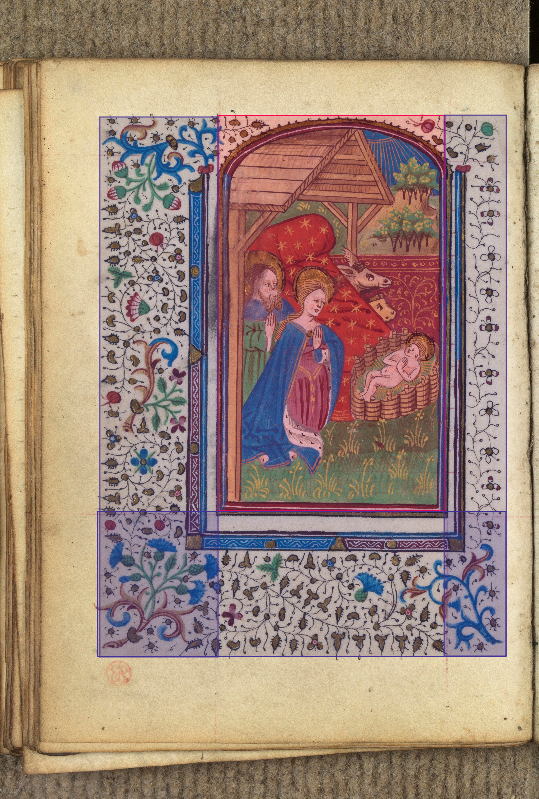
\includegraphics[width=\linewidth, height=7cm, keepaspectratio]{Guidelines/illustration_3.png}
    \caption{a handwritten book of hours with an illustration amidst floral ornamentation.}
    \label{fig:manuscript_bookofhours}
  \end{subfigure}
  \hfill
  \begin{subfigure}{0.48\textwidth}
    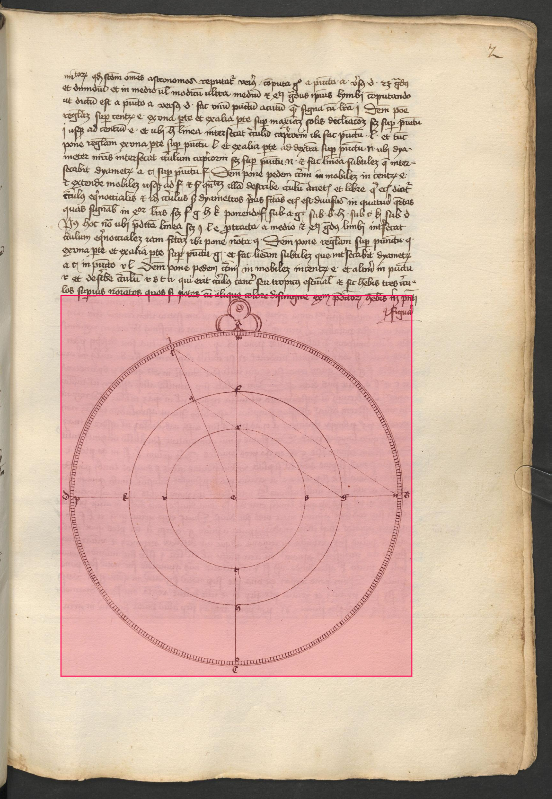
\includegraphics[width=\linewidth, height=7cm, keepaspectratio]{Guidelines/ilustration_5.png}
    \caption{An astronomy manuscript with a mathematical diagrams.}
  \end{subfigure}
  \caption{Illustrations examples}
\end{figure}

\subsubsection{Rules}

The annotations of Illustrations can affected by the layout of the page, they can be grouped and it is hard to understand which ones need to be annotated alone and which ones need to be annotated together.

\begin{itemize}
  \item \textbf{Is there a frame around multiples illustrations ?} : Illustrations in a frame belong together and need to be annotated acordingly. The bounding boxes need to be drawn around the limits of the frame. As shown in this image~\ref{fig:separation}, and shown here~\ref{fig:example_illustration_frame} a grouped illustration without a frame should be separated in multiple annotations. 

  \item \textbf{Is there a common background ?} : If Illustrations share a visual element between them, they need to be annotated together.

  \item \textbf{Do the Illustrations touch ?}: If Illustration touch each other, they need to be annotated together.
\end{itemize}

\begin{figure}
  \centering
  \begin{subfigure}{0.48\textwidth}
    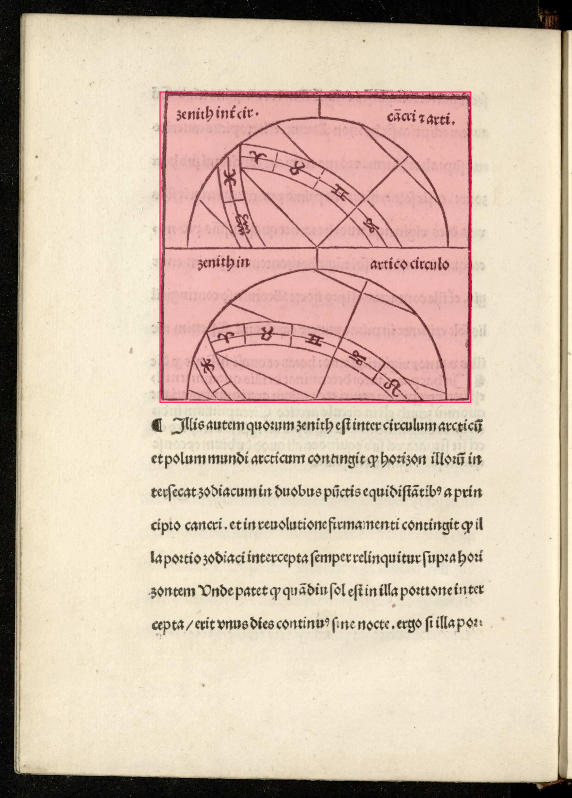
\includegraphics[width=\linewidth, height=7cm, keepaspectratio]{Guidelines/sepsepsep.png}
    \caption{Two illustrations annotated together because they touch and share the same frame.}
    \label{fig:example_illustration_frame}
  \end{subfigure}
  \hfill
  \begin{subfigure}{0.48\textwidth}
    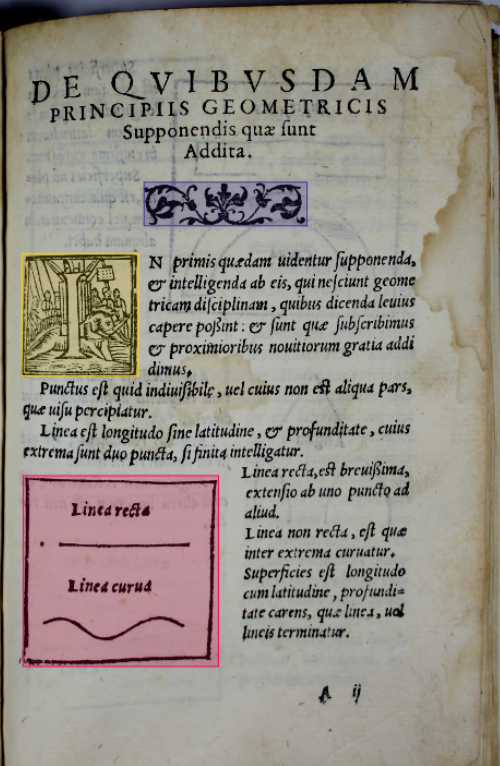
\includegraphics[width=\linewidth, height=7cm, keepaspectratio]{Guidelines/illustration_frame_rule.png}
    \caption{Two illustrations (red) that do not touch but are annotated together because they share a frame.}
    \label{fig:example_illustration_frame_rule}
  \end{subfigure}
  \caption{Edgcases for illustrations}
\end{figure}

\subsubsection{Edgecases}

\begin{itemize}
  \item \textbf{Printer's mark} : A printer's mark is a symbol that was used as a trademark by early printers starting in the 15th century. Printers' marks are often placed on the title page, just below the title and the author's name. The printer's mark should be annotated as an illustration ; see Figure ~\ref{fig:printermark}

  \item \textbf{Illustration and ornamentation} will often be combined into complex visual element. If a visual element is composed by an illustration and an ornamentation, the annotator shoud separate this elements as shown ; see Figures~\ref{fig:manuscript_bookofhours}, \ref{fig:illustration_ornamented_frame} and~\ref{fig:illustration_ornamentation_initial}. 
\end{itemize}


\begin{figure}
  \centering 
  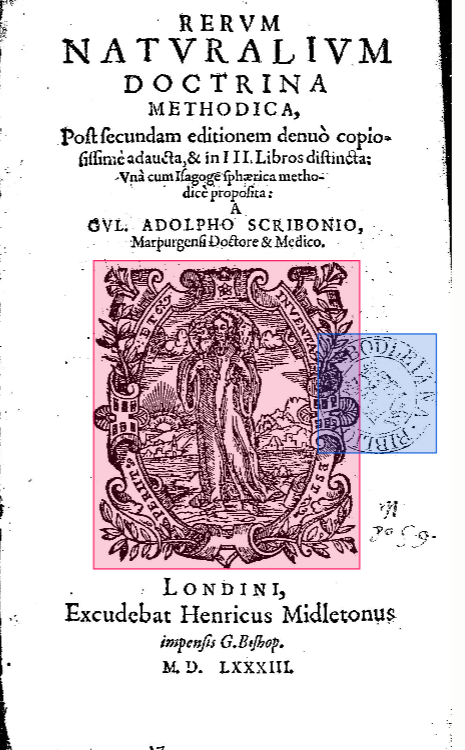
\includegraphics[width=\linewidth, height=7cm, keepaspectratio]{Guidelines/printer_mark.png}
  \caption{A printer's mark on a title page}
  \label{fig:printermark}

\end{figure}



\begin{figure}
  \centering
  \begin{subfigure}{0.48\textwidth}
    \centering
    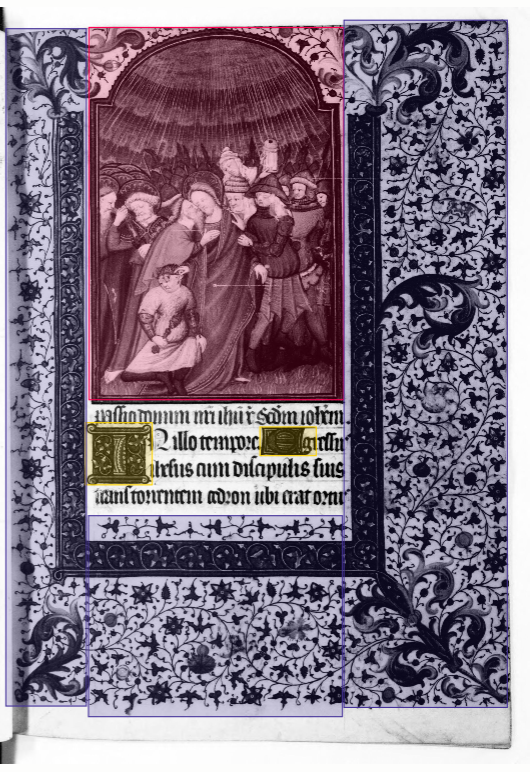
\includegraphics[width=\linewidth, height=7cm, keepaspectratio]{Guidelines/illustration_initial_ornamentation.png}
    \caption{A manuscript that show how to annotate illustration and ornamentation}
    \label{fig:illustration_ornamentation_initial}
  \end{subfigure}
  \hfill
  \begin{subfigure}{0.48\textwidth}
    \centering
    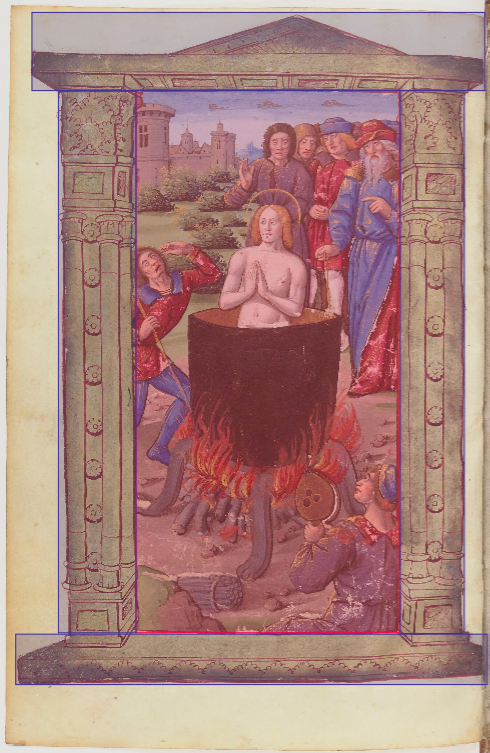
\includegraphics[width=\linewidth, height=7cm, keepaspectratio]{Guidelines/ornamentation_illustration.png}
    \caption{An illustration with an ornamented frame around.}
    \label{fig:illustration_ornamented_frame}
  \end{subfigure}
  \caption{Illustrations and ornaments relationships}
\end{figure}

\subsection{Ornament}\label{section:ornament}
\subsubsection{Description}

An ornament is a graphic element that decorates or embellishes a document without adding informational value.

An ornament is most often an abstract form of illustration, composed of classical patterns (plant ornaments, abstract headpieces, "cul-de-lampe") or repetitive motifs with no meaning other than their intrinsic value as ornaments.

\subsubsection{Rules \& edgecases}

Annotating ornaments is inherently complex, because they frequently interact with and wrap around other elements on the page. Therefore, most ornaments cannot be annotated with a single bounding box. Instead, when an ornament wraps around a visual element (an illustration, a table, a block of text, etc.), it must be \textbf{split into several separate boxes} that follow the contour of the underlying element, rather than being enclosed in one large box that also captures unrelated content.

The following rules apply:

\begin{itemize}
  \item \textbf{The typographic elements for page organization.} (e.g.\ (strokes, bold lines, a simple line or a separator with no complex interaction with the page content) should \textbf{not} be annotated at all.

  \item \textbf{Text inside an ornament} is irrelevant to the annotation: In some manuscripts, there is sometimes text within an ornamental design. Since we are not taking the text into account, these elements must be ornamented normally. Whether or not text appears within the ornamented area does not change how the ornament itself is annotated ; see Figure~\ref{fig:ornament_text}.

  \item \textbf{Ornaments wrapping around another element} must be cut into multiple pieces that follow the shape of that element, instead of a single bounding box ; see Figure~\ref{fig:ornament_1}.

  \item \textbf{Linked/split pieces} resulting from such a cut must be marked with an overlap so that they can later be reconstructed into a single logical ornament ; see Figure~\ref{fig:ornament_overlap}.

  \item \textbf{Ornaments used as separators}, for instance to delimit illustrations or tables from one another, should be annotated as ornaments in their own right ; see Figure~\ref{fig:ornament_tables}.
\end{itemize}

\begin{figure}
  \centering
  \begin{subfigure}{0.48\textwidth}
    \centering
    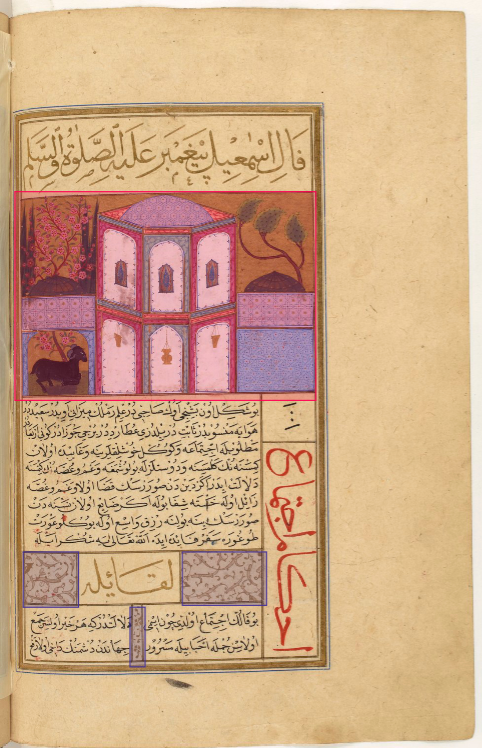
\includegraphics[width=\linewidth, height=7cm, keepaspectratio]{Guidelines/ornament.png}
    \caption{example of ornaments annotations}
    \label{fig:ornament_1}
  \end{subfigure}
  \hfill
    \begin{subfigure}{0.48\textwidth}
    \centering
    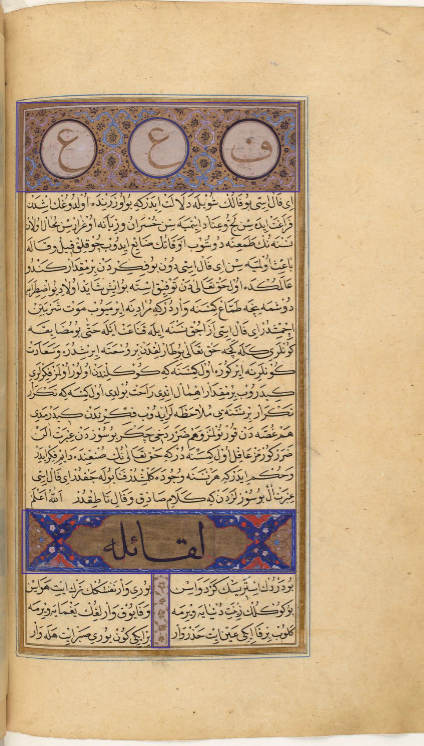
\includegraphics[width=\linewidth, height=7cm, keepaspectratio]{Guidelines/ornament_2.png}
    \caption{We do not care if there is text inside of the ornamentation.}
    \label{fig:ornament_text}
  \end{subfigure}
  \hfill
  \begin{subfigure}{0.48\textwidth}
    \centering
    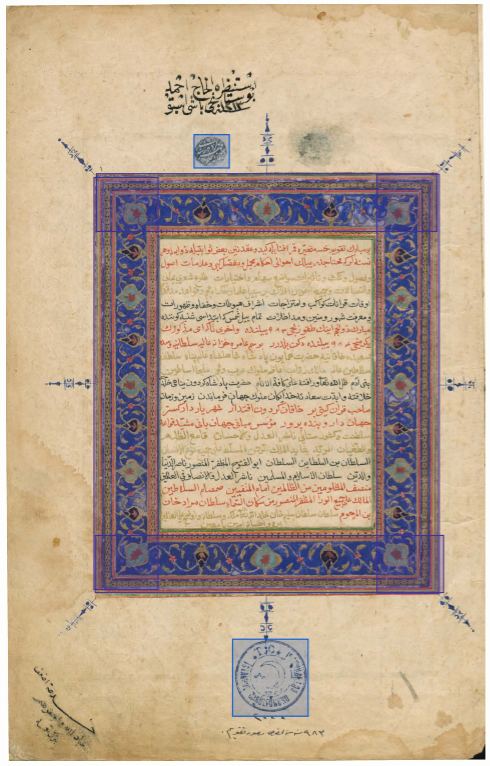
\includegraphics[width=\linewidth, height=7cm, keepaspectratio]{Guidelines/ornament_3.png}
    \caption{When cutting out ornamentation, pieces that are linked together should be marked with overlays so that they can be reconstructed later.}
    \label{fig:ornament_overlap}
  \end{subfigure}
  \hfill
  \begin{subfigure}{0.48\textwidth}
    \centering
    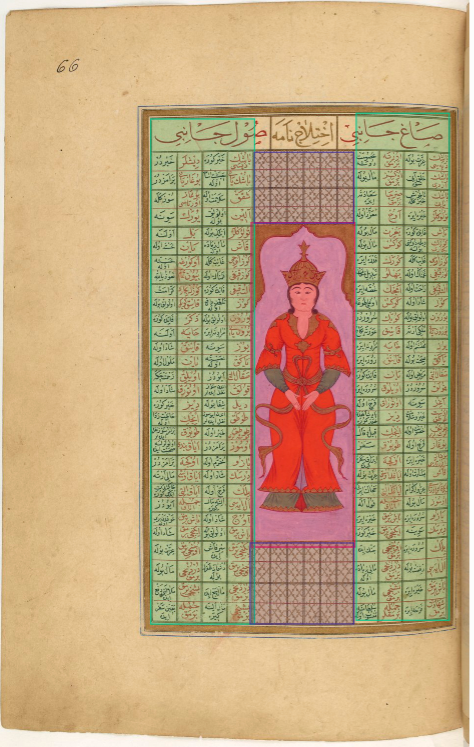
\includegraphics[width=\linewidth, height=7cm, keepaspectratio]{Guidelines/ornament_4.png}
    \caption{Ornamention can be used to separate element like illustrations or tables.}
    \label{fig:ornament_tables}
  \end{subfigure}
  \hfill  
  \begin{subfigure}{0.48\textwidth}
    \centering
    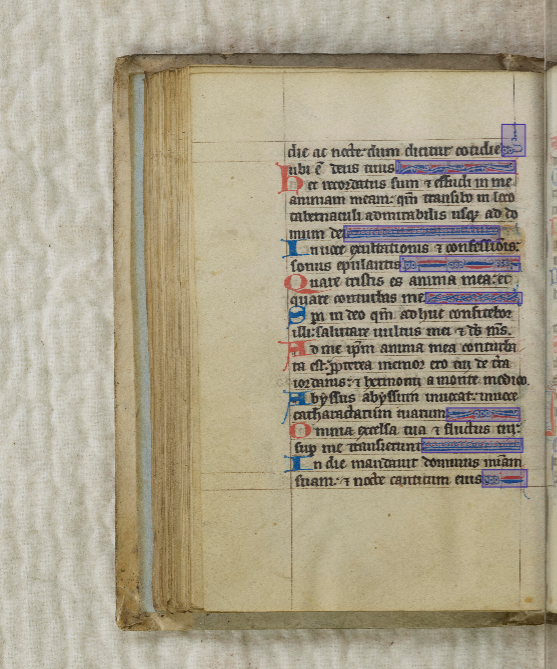
\includegraphics[width=\linewidth, height=7cm, keepaspectratio]{Guidelines/ornament_end_of_line.png}
    \caption{In manuscript, the end of the line can be ornemented}
    \label{fig:ornament_end_of_line}
  \end{subfigure}
  \hfill  
  
  \caption{ornaments examples}
\end{figure}


\subsection{Initial}
\subsubsection{Description}

In a written or manuscript work, an initial is a letter at the beginning of a word, a chapter, or a paragraph that is larger than the rest of the text. An initial is often several lines in height, and, in older books or manuscripts, may take the form of an historiated initial.

\begin{figure}
  \centering
  \begin{subfigure}{0.48\textwidth}
    \centering
    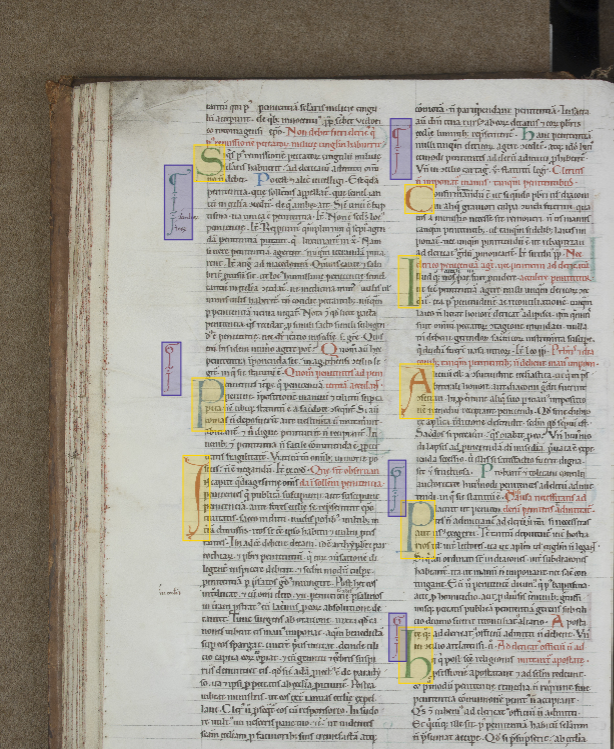
\includegraphics[width=\linewidth, height=7cm, keepaspectratio]{Guidelines/initial.png}
    \caption{example of initials annotations}
    \label{fig:initial_1}
  \end{subfigure}
  \hfill
  \begin{subfigure}{0.48\textwidth}
    \centering
    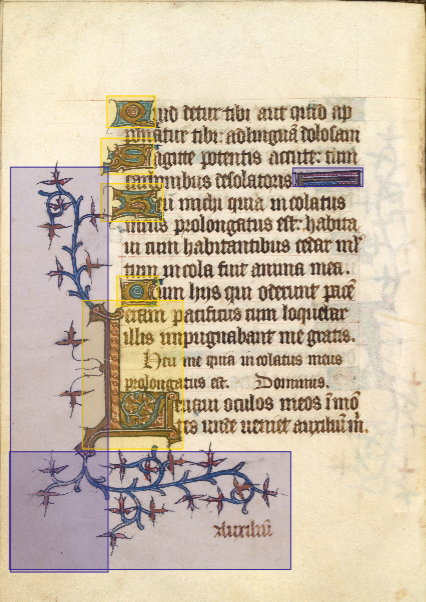
\includegraphics[width=\linewidth, height=7cm, keepaspectratio]{Guidelines/lettrine_ornament.png}
    \caption{Example of the relationship between the initial letter and the ornamentation and how to annotate them.}
    \label{fig:initial_ornament}
  \end{subfigure}
  \hfill
  \begin{subfigure}{0.48\textwidth}
    \centering
    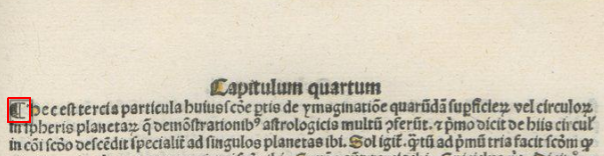
\includegraphics[width=\linewidth, height=7cm, keepaspectratio]{Guidelines/pilcrown_printed.png}
    \caption{Example of a printed pilcrow (¶).}
    \label{fig:printed_pilcrow}
  \end{subfigure}
  \hfill
  \begin{subfigure}{0.48\textwidth}
    \centering
    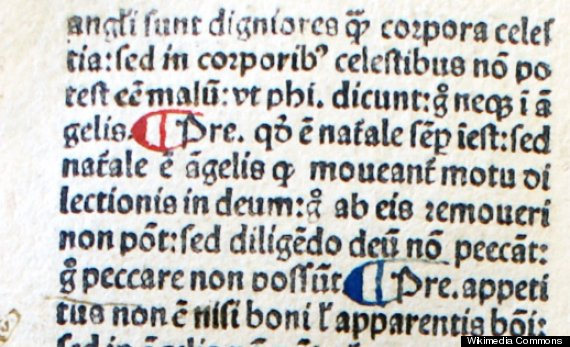
\includegraphics[width=\linewidth, height=7cm, keepaspectratio]{Guidelines/manuscript_pilcrow.jpg}
    \caption{Example of a manuscript pilcrow (¶).}
    \label{fig:manuscript_pilcrow}
  \end{subfigure}
  \hfill
  \caption{Example of initials}
\end{figure}

\subsubsection{Rules}

  An initial is annotated as such only if it is \textbf{visually distinguishable from the body text} typically by a significantly larger size (spanning at least two lines of the surrounding text), a different script, color, or decorative treatment. A letter that is only slightly enlarged compared to the running text should not be annotated as an initial ; see Figure~\ref{fig:both_page}.

\subsubsection{Edgecases}

Initials are letters and therefore can be tricky to annotate due to their textual nature.

\begin{itemize}
  \item \textbf{Initial letter can be used in manuscripts as a basis for marginal ornamentation}. We annotate the initial letter in a "cautious" manner, limiting ourselves to the actual initial letter, and we annotate the rest of the ornamentation using the ornamentation class ; see Figures~\ref{fig:main_page} and \ref{fig:illustration_ornamentation_initial}.

  \item \textbf{Initial capitals can be confused with the paragraph mark (pilcrow ¶)} frequently used in manuscripts. Often written in ink of a different color than the text (red), the pilcrow should not be annotated like an initial capital ; see Figures~\ref{fig:printed_pilcrow}, \ref{fig:manuscript_pilcrow}.
\end{itemize}

\subsection{Stamp}

Stamps are marks that identify the institutions that hold or held the documents (libraries, archives). These markings are not all the same depending on the document and the date they were applied to the work. For bound documents (books, manuscripts, albums), the stamp is on the first page. For a stack of unbound documents, each loose page will be stamped. 

\begin{figure}
  \centering
  \begin{subfigure}{0.48\textwidth}
    \centering
    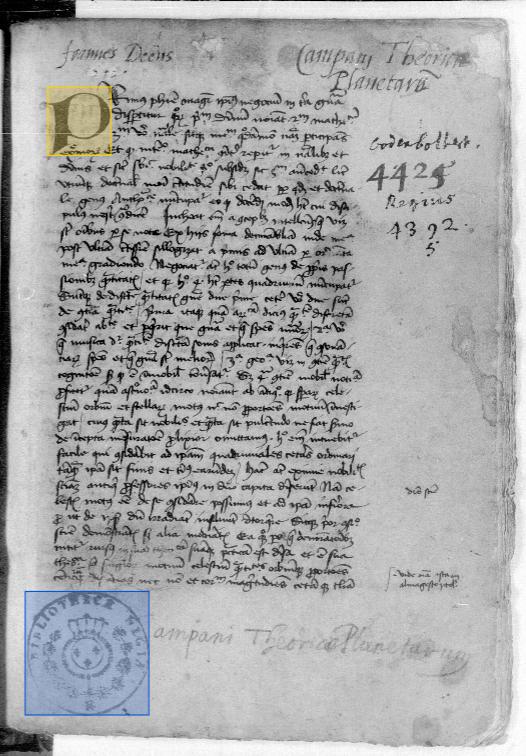
\includegraphics[width=\linewidth, height=7cm, keepaspectratio]{Guidelines/stamp_ex_libris.png}
    \caption{example of a stamp covering his old bookplate.}
    \label{fig:stamp_ex_libris}
  \end{subfigure}
  \hfill
  \begin{subfigure}{0.48\textwidth}
    \centering
    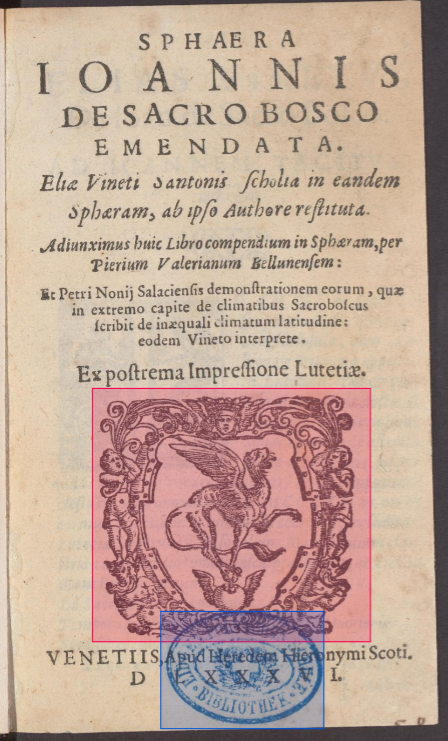
\includegraphics[width=\linewidth, height=7cm, keepaspectratio]{Guidelines/stamps.png}
    \caption{example of a stamp on a title page.}
    \label{fig:stamp_1}
  \end{subfigure}
  \hfill
  \begin{subfigure}{0.48\textwidth}
    \centering
    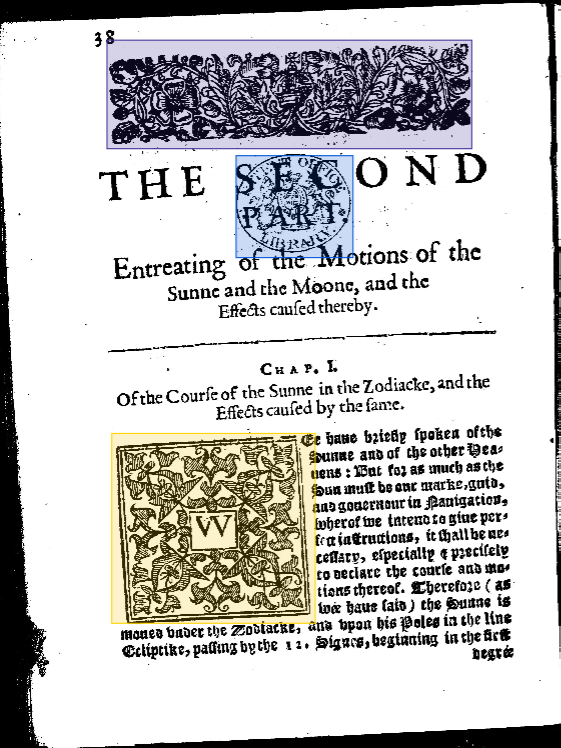
\includegraphics[width=\linewidth, height=7cm, keepaspectratio]{Guidelines/stamps_2}
    \caption{example of a stamp on a first page.}
    \label{fig:stamp_2}
  \end{subfigure}
  \hfill
  \begin{subfigure}{0.48\textwidth}
    \centering
    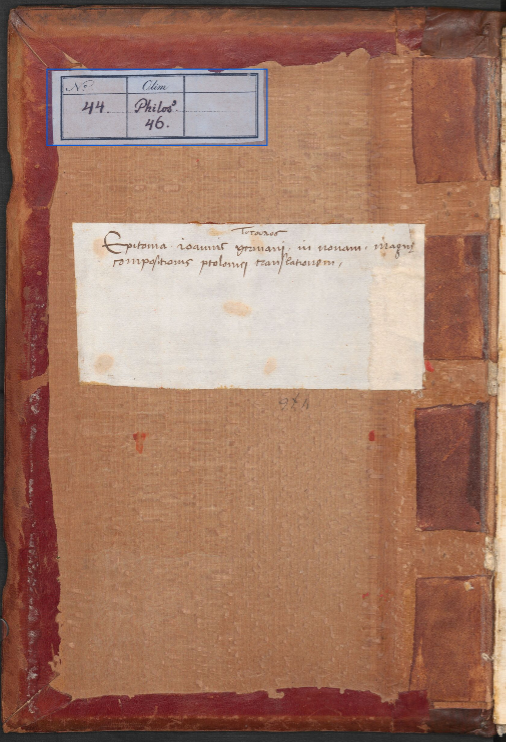
\includegraphics[width=\linewidth, height=7cm, keepaspectratio]{Guidelines/library_stamp.png}
    \caption{example of a library label}
    \label{fig:label}
  \end{subfigure}
  \hfill
  \caption{Example of stamps and library labels}
\end{figure}

\subsubsection{Rules}

\begin{itemize}
  \item \textbf{Annotate all visible stamps}: manuscripts and old books in France have moved between several librairies and therefore often have several stamps which need to be annotated ; see Figure~\ref{fig:stamp_1} and \ref{fig:stamp_2}.

  \item \textbf{Ex-Libris }: Before the widespread use of the stamp, book owners used a handwritten Ex-Libris on the title page; this phrase should not be annotated as a stamp even if it serves the same purpose ; see Figure~\ref{fig:stamp_ex_libris}.

  \item In addition to library stamps, the stamp class is also used to annotate library labels ; see Figure~\ref{fig:label}.
\end{itemize}

\subsection{Table}

A table is an arrangement of information or data, usually in rows and columns, or possibly according to a more complex structure. 

For tables, the header and the footer must included in the annotation if it is present. 

\subsubsection{Rules}

\begin{itemize}
  \item \textbf{The bounding box must include the entire table structure}, including the \textbf{header and footer} rows if present, as well as any surrounding \textbf{border or frame} that is part of the table itself ; see Figure~\ref{fig:tabula_with_title}.

  \item If the table has a \textbf{title or caption} that is graphically separated from the table body (e.g.\ placed above or below it, not enclosed by the table's border), it should \textbf{not} be included in the annotation ; only the tabular structure itself is annotated ; see Figure~\ref{fig:tabula_initial}.

  \item Tables with \textbf{non-rectangular or non-linear structure} (e.g.\ circular tables, radial diagrams used to present structured information such as genealogies or calendars) must still be annotated as tables, using a bounding box that encloses the full extent of the structure.

  \item If a page contains \textbf{several distinct tables} (not visually merged and separated by clear spacing, text, or ornamentation), each table should be annotated separately, even if they share the same overall topic or are placed side by side : see Figure~\ref{fig:tabula_ornement}.

  \item If a table is \textbf{split across a page break or a column break} but is visually one continuous table (repeated headers, continued numbering, etc.), each visible portion is annotated as a separate instance, since annotation is done per visible bounding region.
\end{itemize}

\subsubsection{Edgecases}

\begin{itemize}
  \item \textbf{Tables can be difficult to distinguish from simple lists or aligned text} (e.g.\ an index, a table of contents, or enumerated items with aligned page numbers). A table should only be annotated when there is a clear multi-column/multi-row structure with at least two dimensions of organization ; a single column of aligned entries should not be annotated as a table.

  \item \textbf{Tables can be enclosed or decorated with ornamentation} (borders, frames, or historiated elements). In this case, only the tabular content and its structural border are annotated as a table ; any additional decorative ornamentation surrounding it should be annotated separately using the ornamentation class, following the same logic as for illustrations (see Section~\ref{section:ornament}).

  \item \textbf{Tables with a circular or radial representation} of information (frequent in historical documents, e.g.\ astronomical or genealogical diagrams) should be annotated as tables rather than as illustrations, even though they may visually resemble diagrams or figures.

  \item \textbf{Indexes} and content tables should not be annotated.
\end{itemize}

\begin{figure}
  \centering
  \begin{subfigure}{0.48\textwidth}
    \centering
    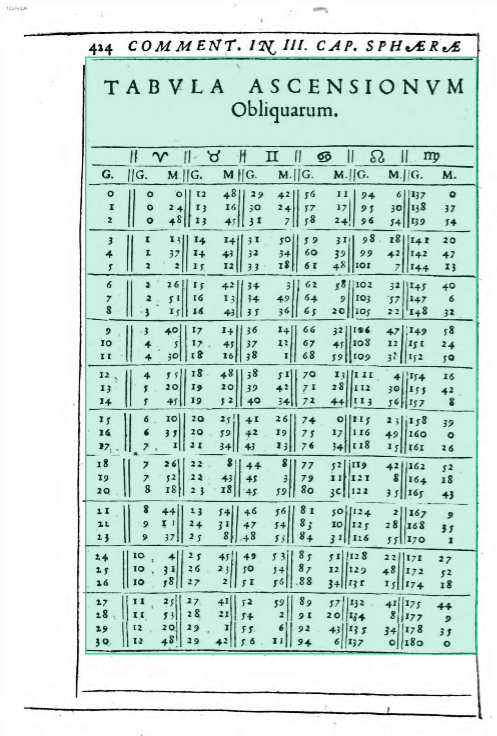
\includegraphics[width=\linewidth, height=7cm, keepaspectratio]{Guidelines/table_1.png}
    \caption{example of an annotated tablewith title}
    \label{fig:tabula_with_title}
  \end{subfigure}
  \hfill
  \begin{subfigure}{0.48\textwidth}
    \centering
    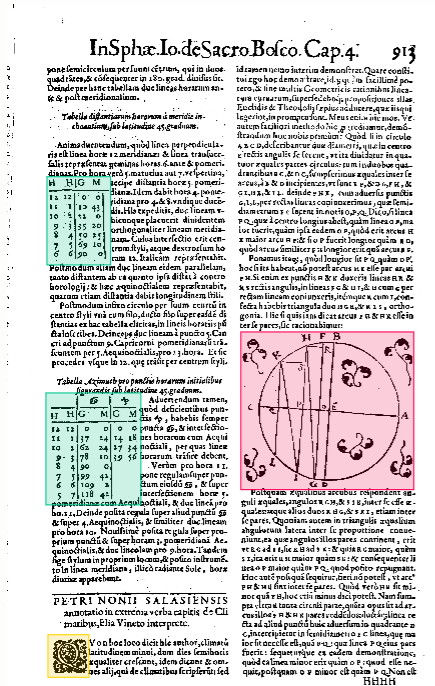
\includegraphics[width=\linewidth, height=7cm, keepaspectratio]{Guidelines/table_2.png}
    \caption{example of tables inserted into the text .}
    \label{fig:tabula_text}
  \end{subfigure}
  \hfill
  \begin{subfigure}{0.48\textwidth}
    \centering
    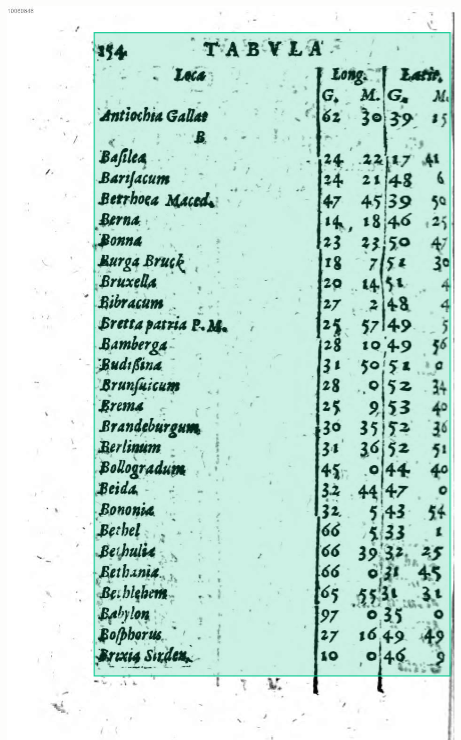
\includegraphics[width=\linewidth, height=7cm, keepaspectratio]{Guidelines/table_3.png}
    \caption{example of a table.}
    \label{fig:tabula_example}
  \end{subfigure}
  \hfill
  \begin{subfigure}{0.48\textwidth}
    \centering
    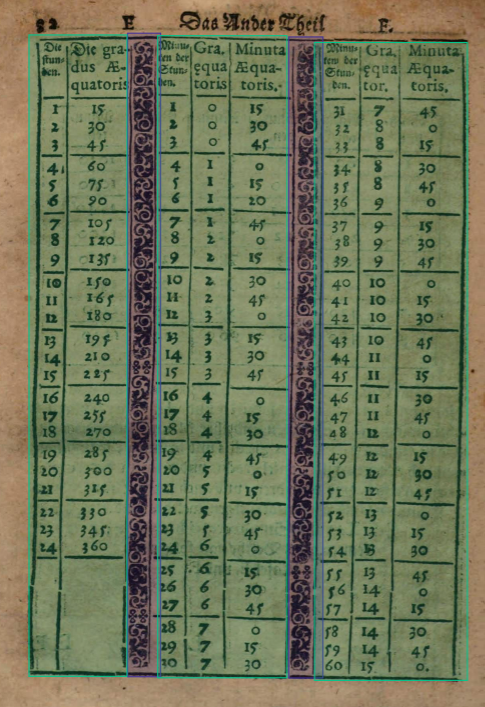
\includegraphics[width=\linewidth, height=7cm, keepaspectratio]{Guidelines/table_6.png}
    \caption{example of tables with ornement.}
    \label{fig:tabula_ornement}
  \end{subfigure}
  \hfill
  \begin{subfigure}{0.48\textwidth}
    \centering
    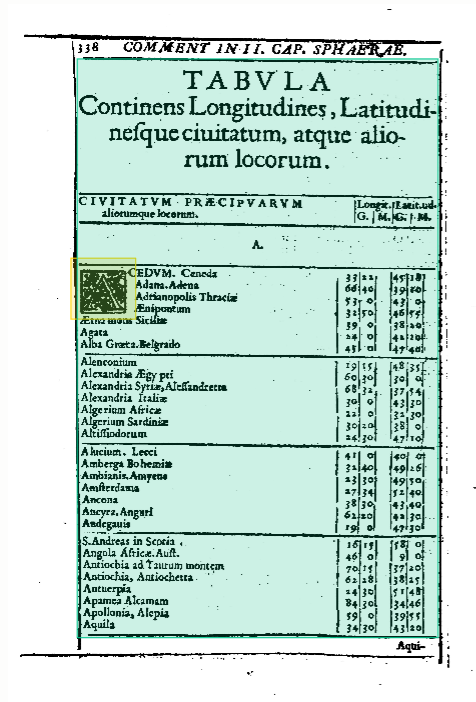
\includegraphics[width=\linewidth, height=7cm, keepaspectratio]{Guidelines/table_7.png}
    \caption{example of a a table with an initial.}
    \label{fig:tabula_initial}
  \end{subfigure}
  \hfill
  \caption{Example of tables}
\end{figure}

 
 



\chapter[Annexes : Expériences]{Expérience : Évaluation des capacités d'annotation de \gls{vlm} en \textit{zero shot}}

L'objectif de cette expérience était d'évaluer rapidement les capacités de ces nouvelles technologies afin d'en identifier clairement les forces et les limites. Pour ce faire, le prompt ci-dessous a été utilisé pour comparer et analyser les réponses de trois \gls{vlm} différents dans des conditions identiques.

\begin{quote}
	
	\textit{Je fais une expérience sur les VLM et leur capacité à annoter des images historiques en zero-shot / few-shot.}
	
	\textit{Les classes à détecter sont :}
	
	\begin{itemize}
		\item \textit{Illustrations (imprimés et manuscrites)}
		
		\item \textit{lettrines}
		
		\item \textit{estampilles de bibliothèques}
		
		\item \textit{ornementations}
		
		\item \textit{tables (tableaux numériques)}
	\end{itemize}
	
	\textit{Voici une image d'un livre imprimé historique, produis soit un fichier txt avec les coordonnées yolo des classes que tu détectes, soit un masque de segmentation par pixel qui segmente les classes que tu détectes.}
	\label{anx:prompt}	
\end{quote}

\begin{figure}[h]
	\centering
	\caption{résultats pour \textit{Claude Sonnet 5 Moyen}}
	\begin{subfigure}{0.45\textwidth}
		\centering
		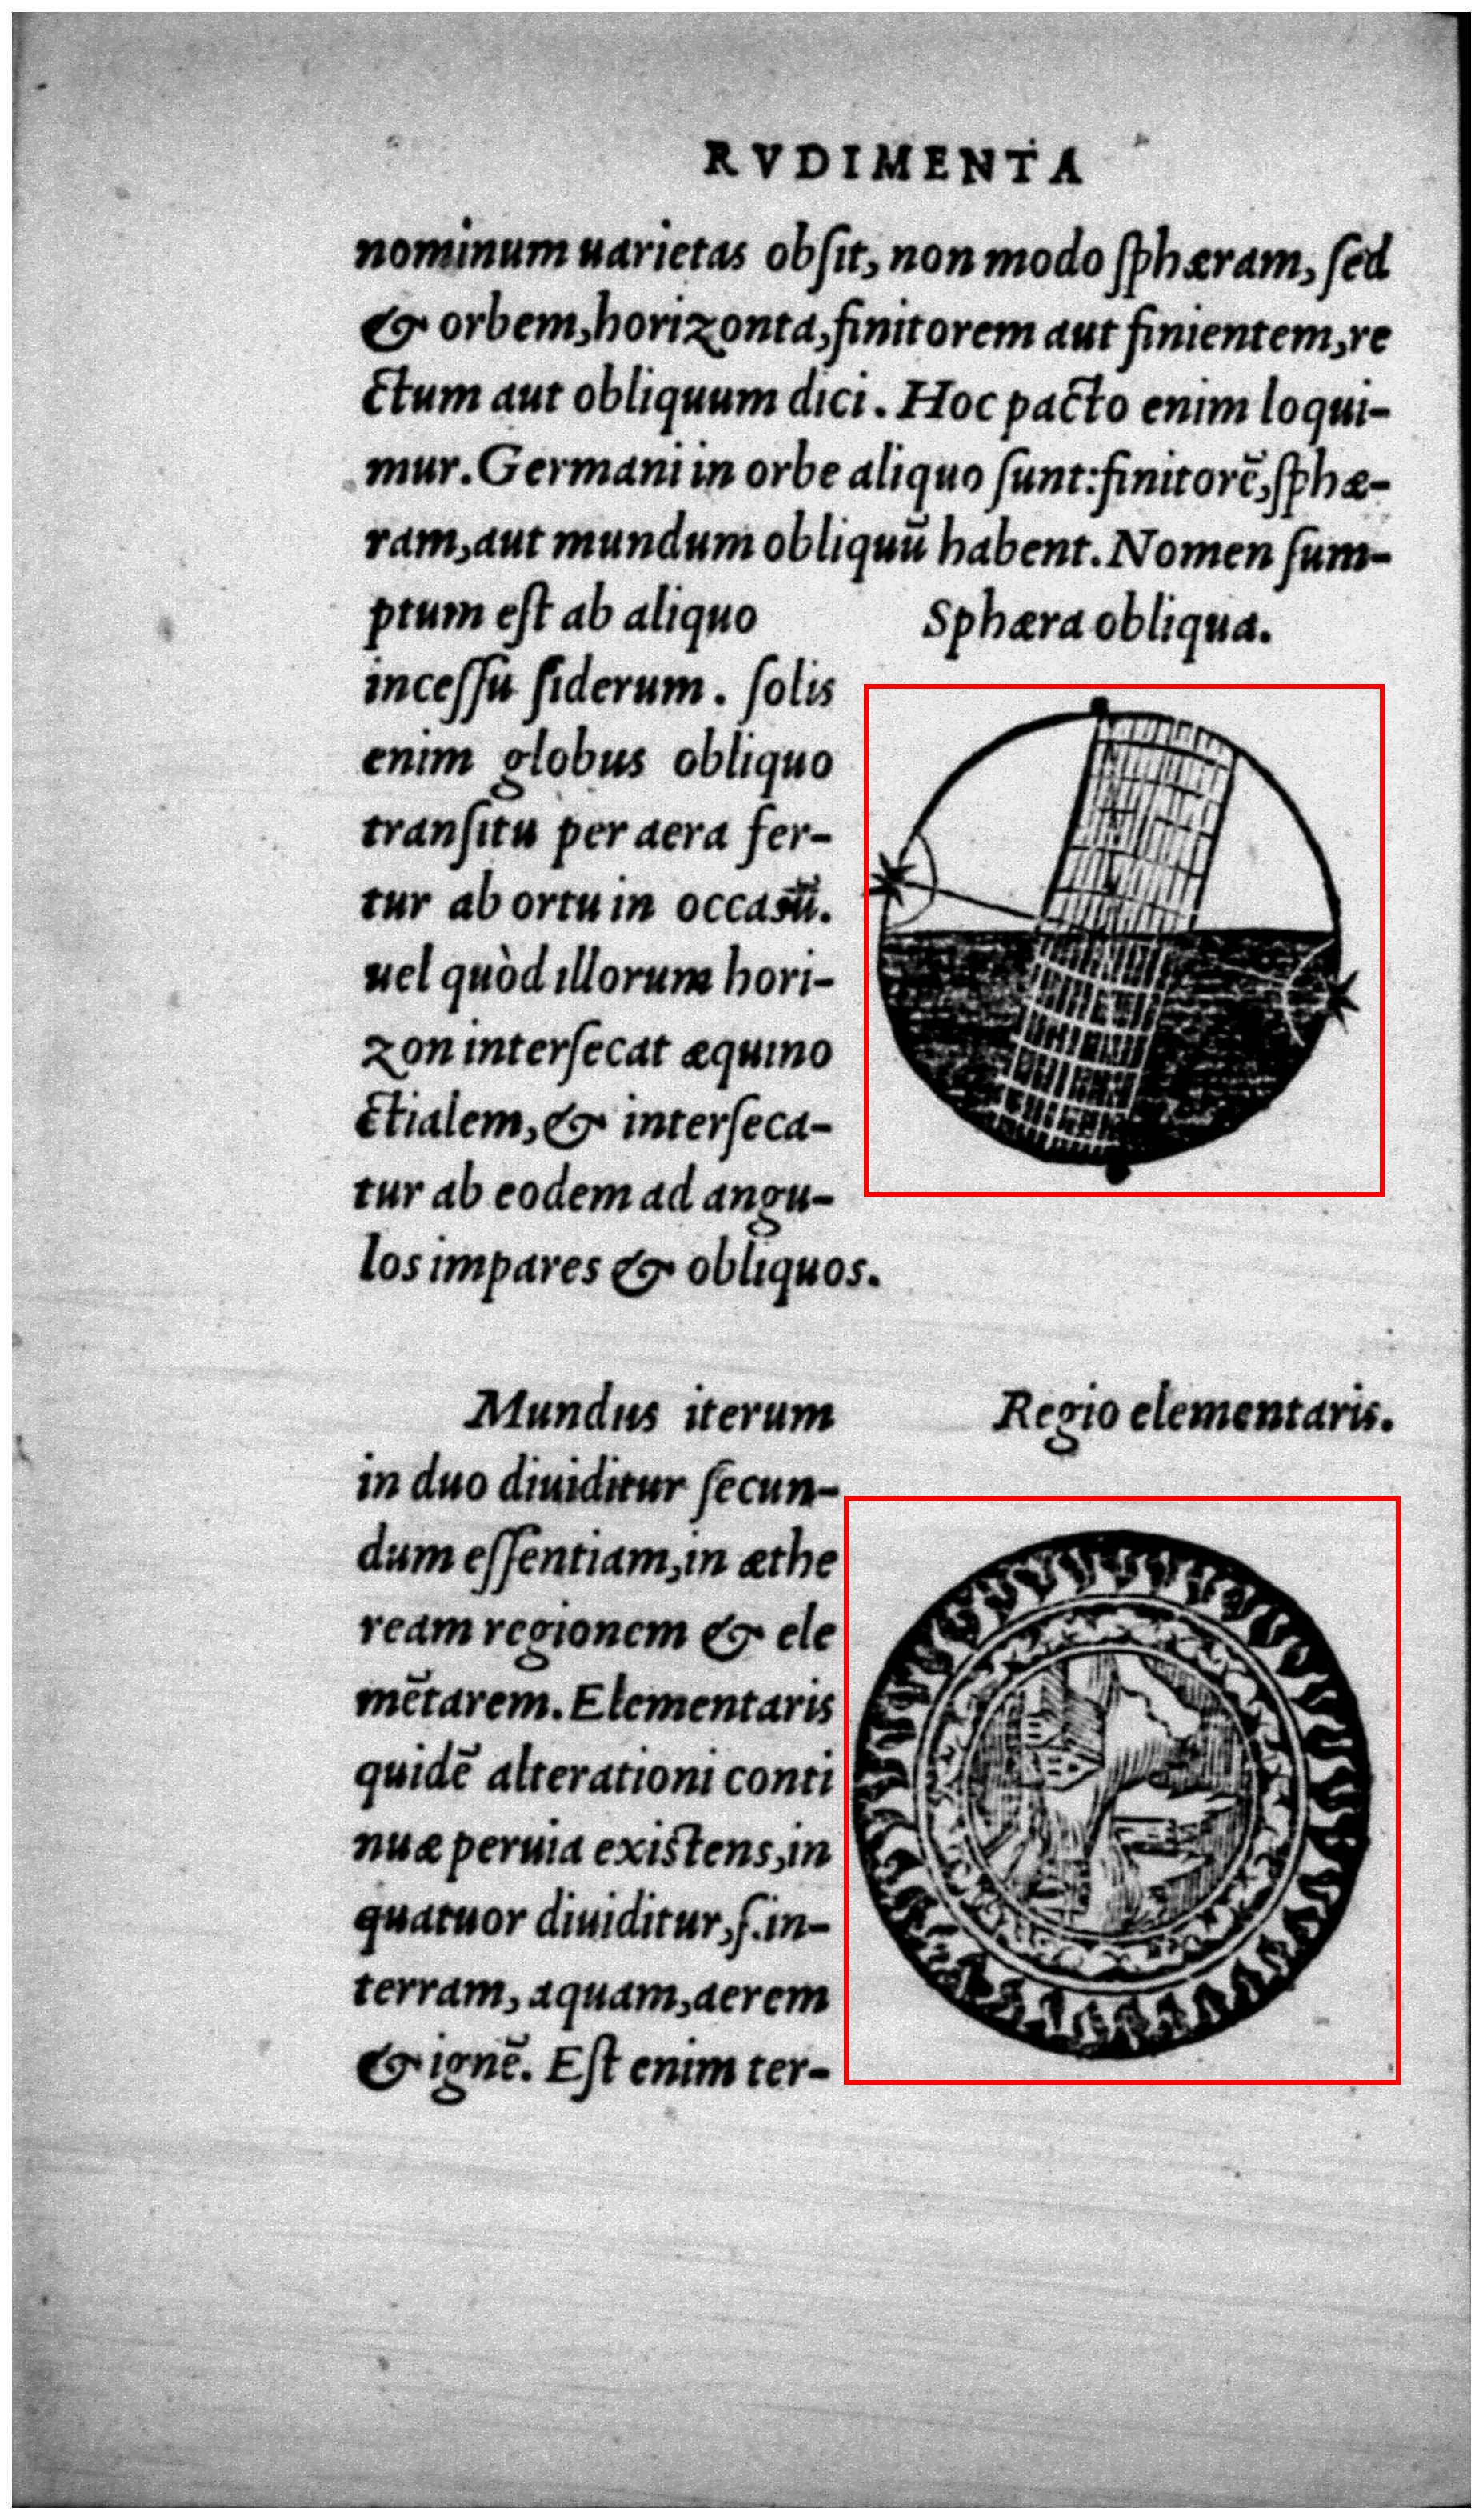
\includegraphics[height=5.5cm]{img/illustrationsonnet5zeroshot.jpg}
		\caption{Tache de détection d'illustration sur une image du jeu S-VED}
		
	\end{subfigure}
	\hfill
	\begin{subfigure}{0.45\textwidth}
		\centering
		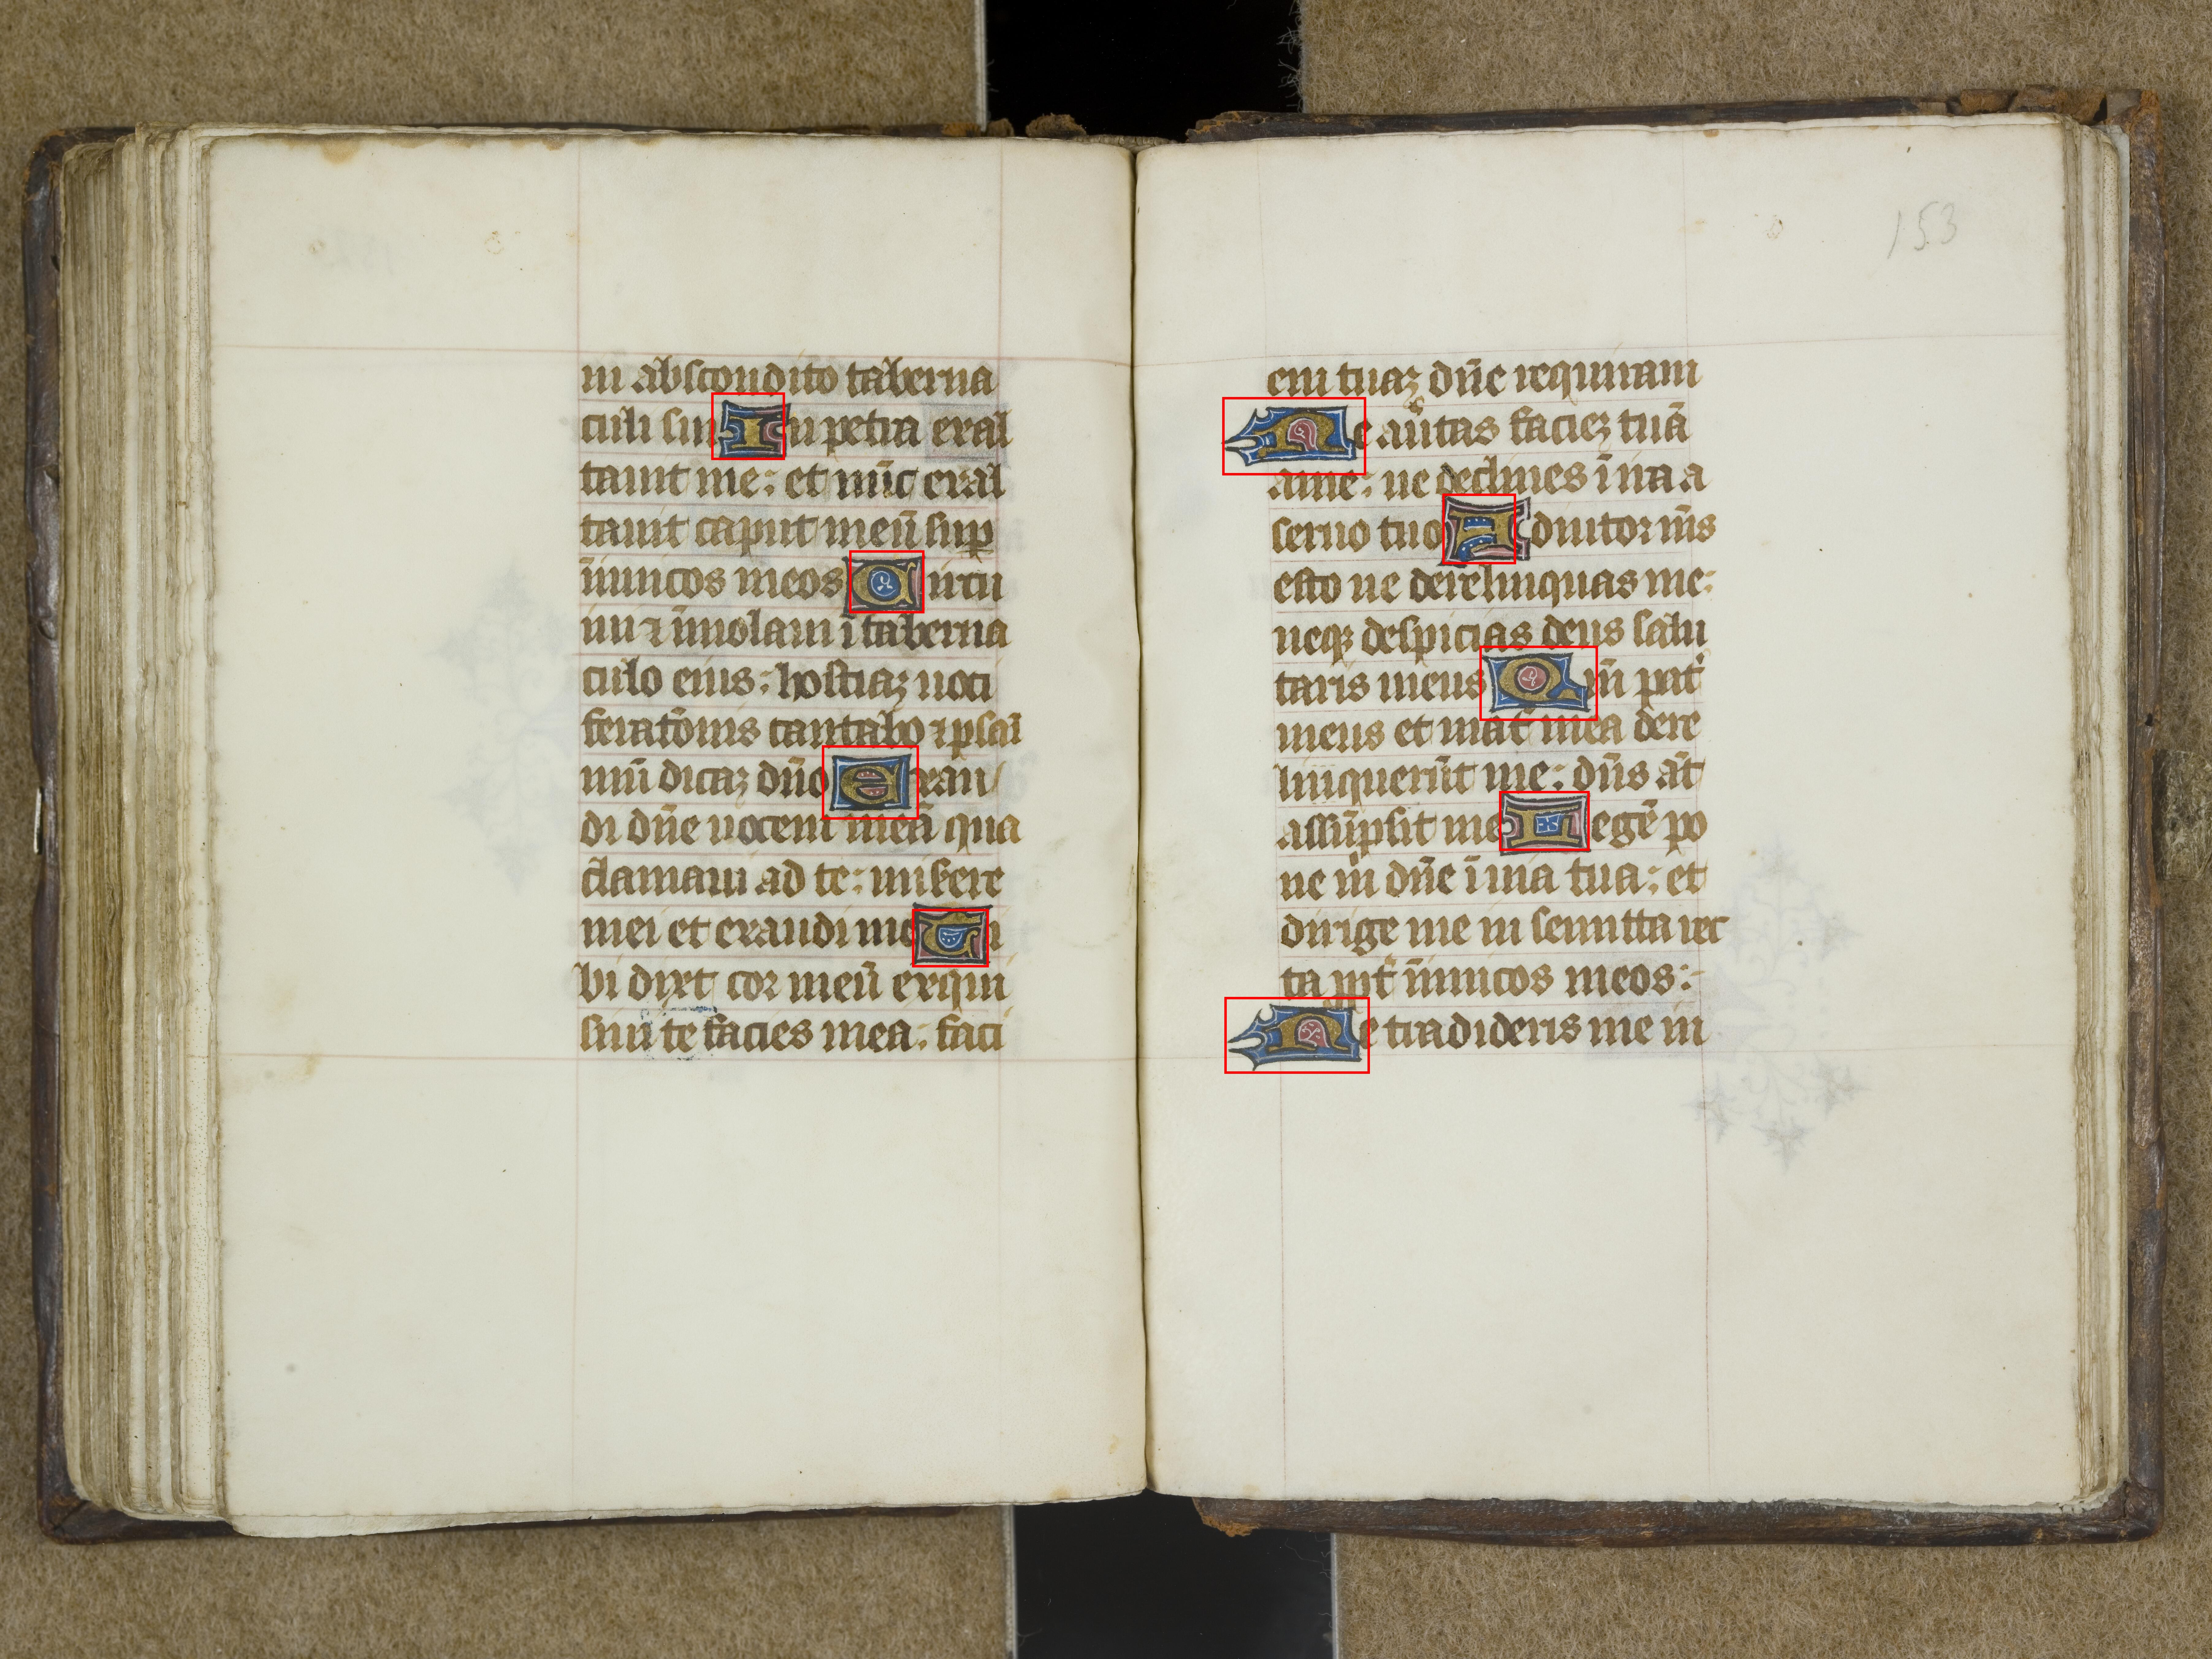
\includegraphics[height=5.5cm]{img/lettrinesonnet5zeroshot.jpg}
		\caption{Tache de détection de lettrine sur une image du jeu Horae}
	\end{subfigure}
	
	\begin{subfigure}{0.45\textwidth}
		\centering
		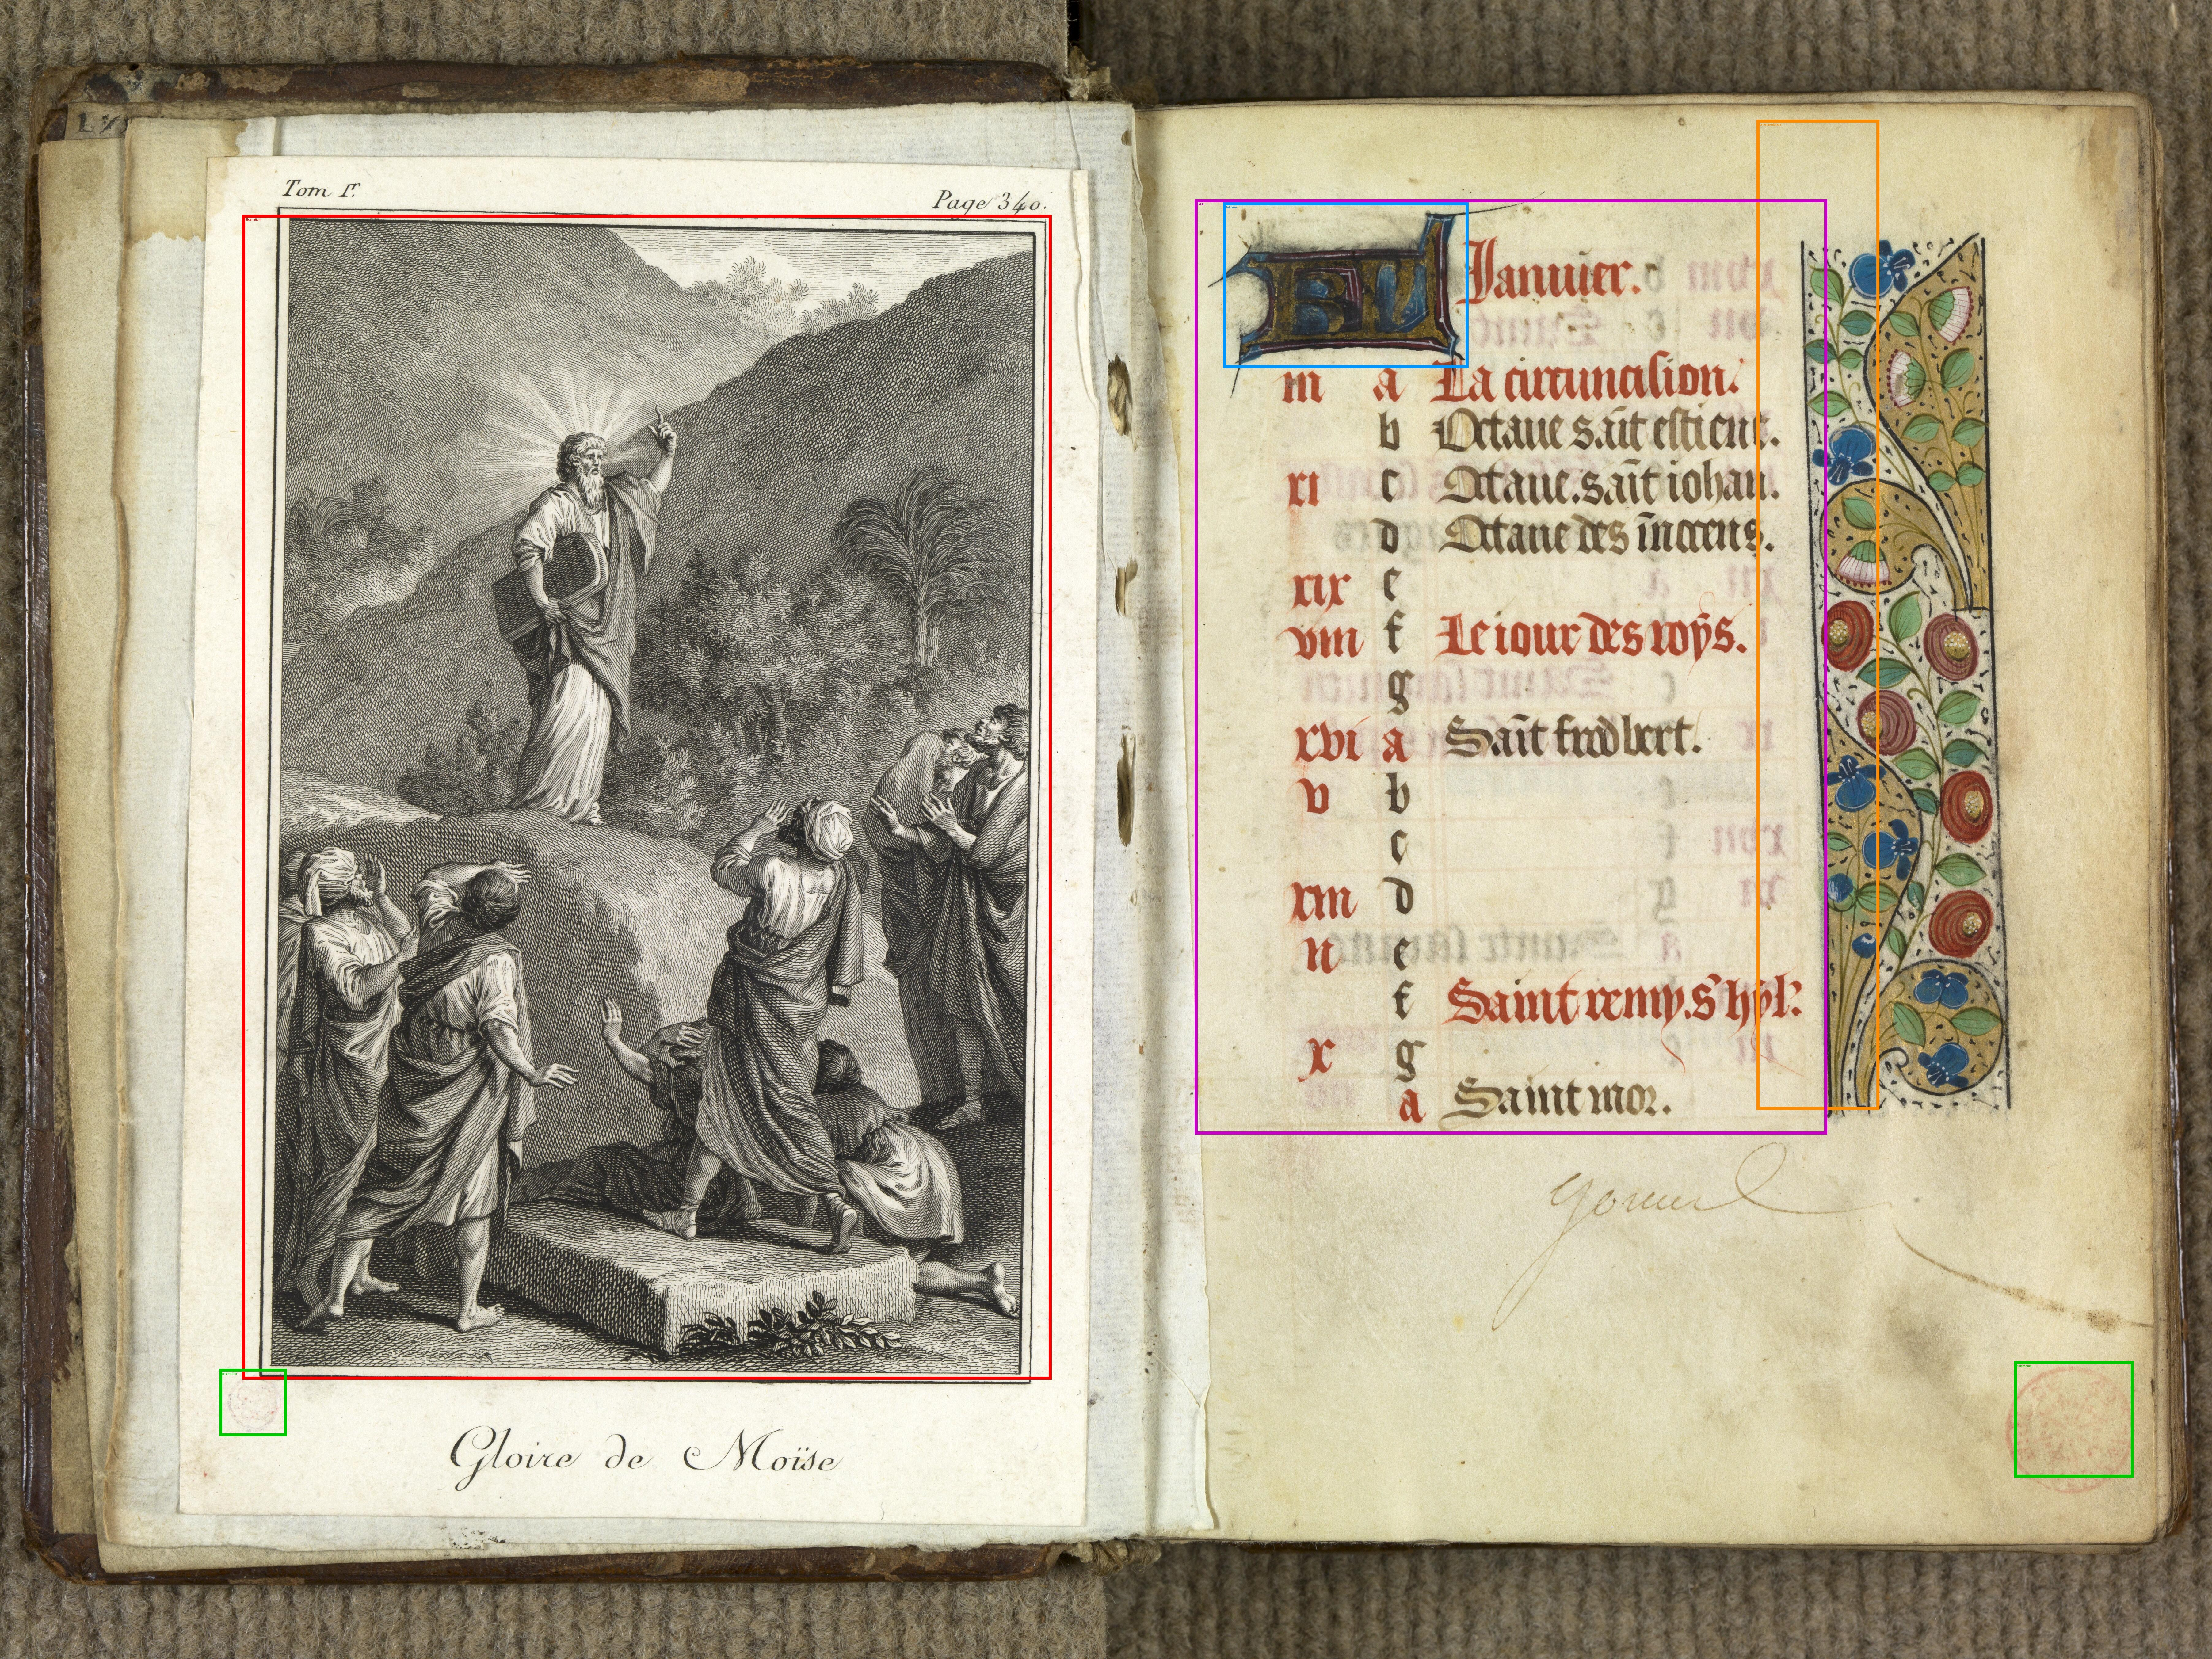
\includegraphics[height=6cm]{img/multiclassesonnet5zeroshot.jpg}
		\caption{Tache de détection multiclasse sur une image du jeu Horae. On notera que le modèle applique la classe \textit{table} au calendrier.}
	\end{subfigure}
\end{figure}

\begin{figure}[h]
	\centering
	\caption{résultats pour \textit{GPT-5.6 Luna}}
	\begin{subfigure}{0.45\textwidth}
		\centering
		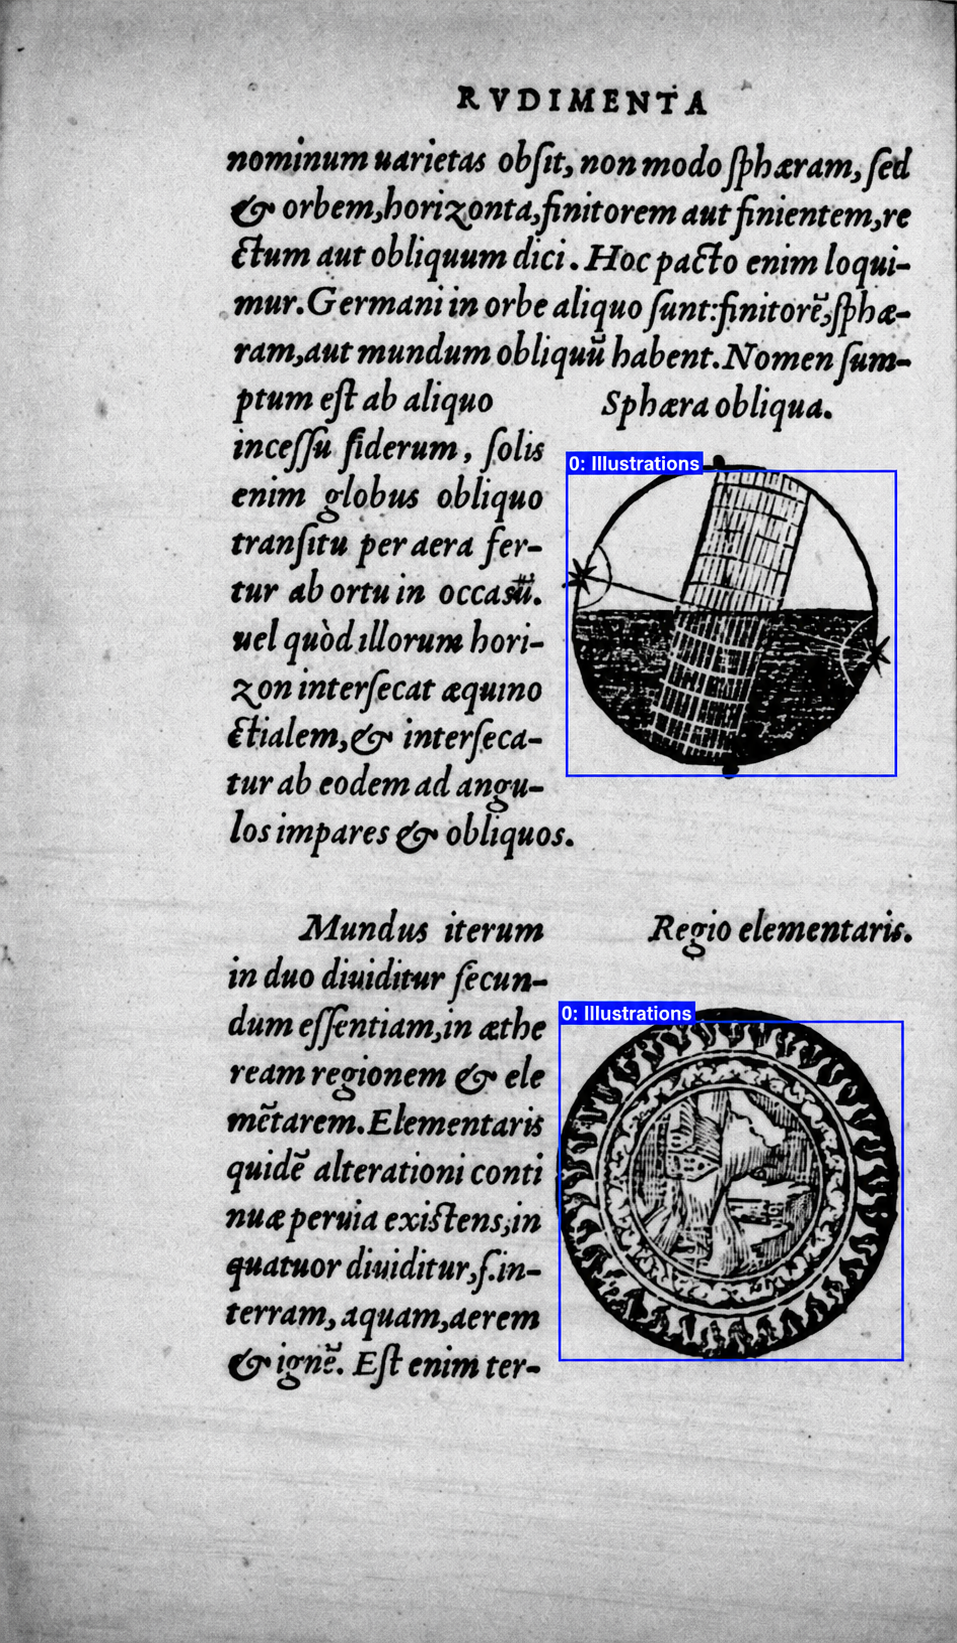
\includegraphics[height=5.5cm]{img/chatgpt1.png}
		\caption{Tache de détection d'illustration sur une image du jeu S-VED}
		
	\end{subfigure}
	\hfill
	\begin{subfigure}{0.45\textwidth}
		\centering
		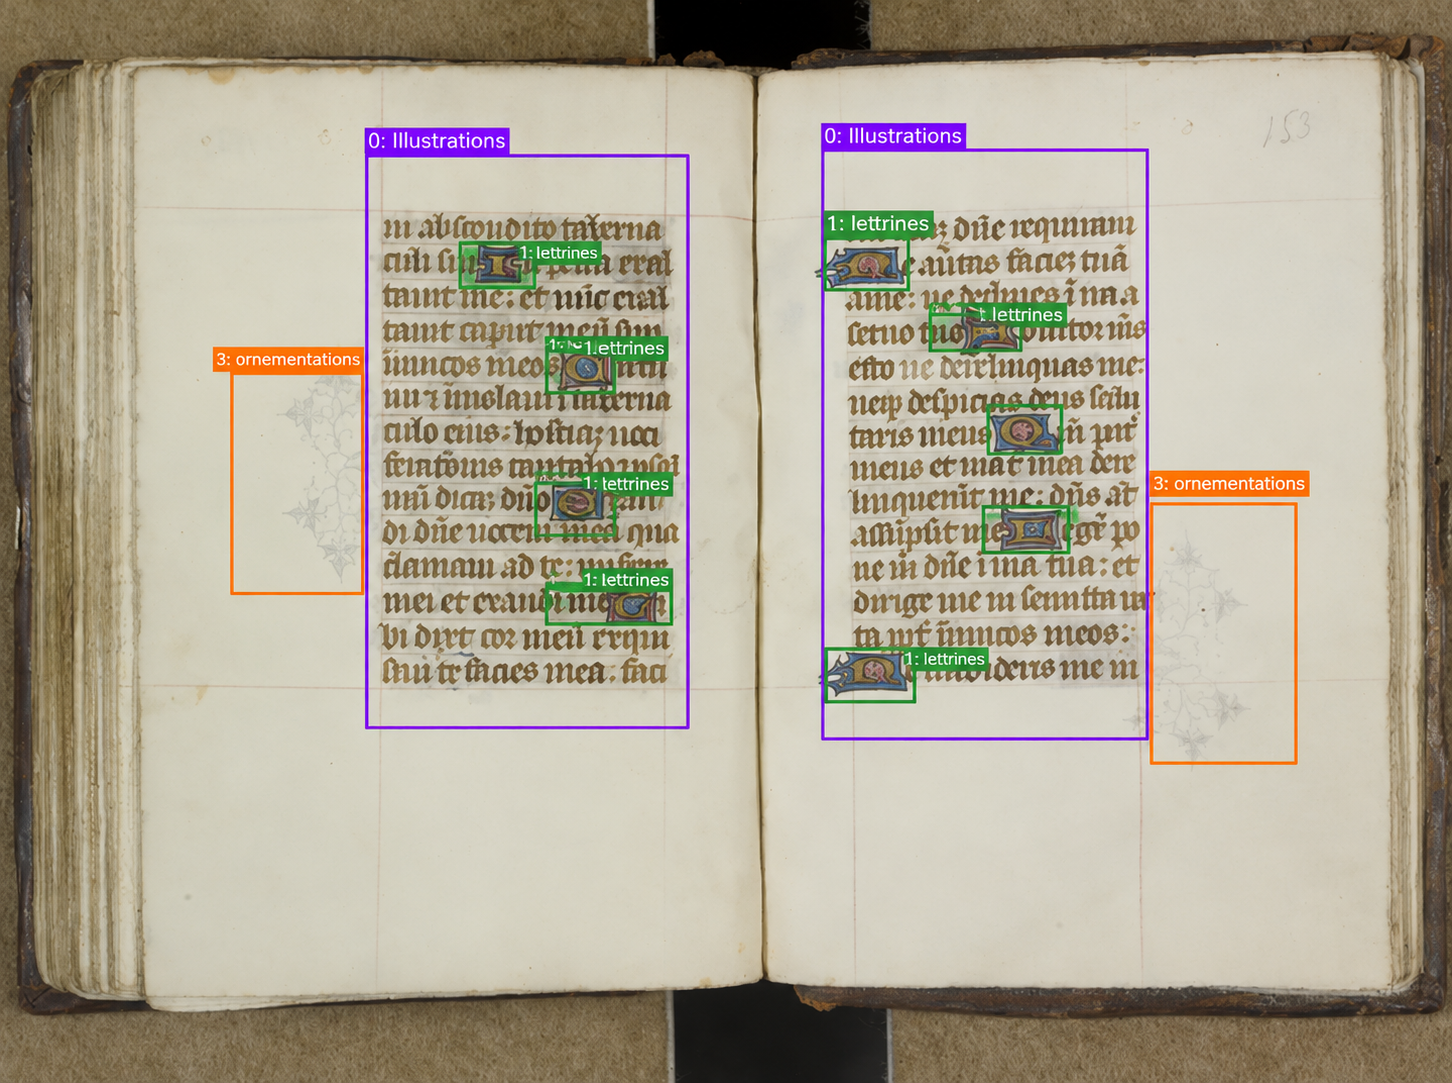
\includegraphics[height=5.5cm]{img/chatgpt3.png}
		\caption{Tache de détection de lettrine sur une image du jeu Horae. Les boîtes englobantes des lettrines sont insufissantes et le modèle détecte le texte comme une illustration.}
	\end{subfigure}
	
	\begin{subfigure}{0.45\textwidth}
		\centering
		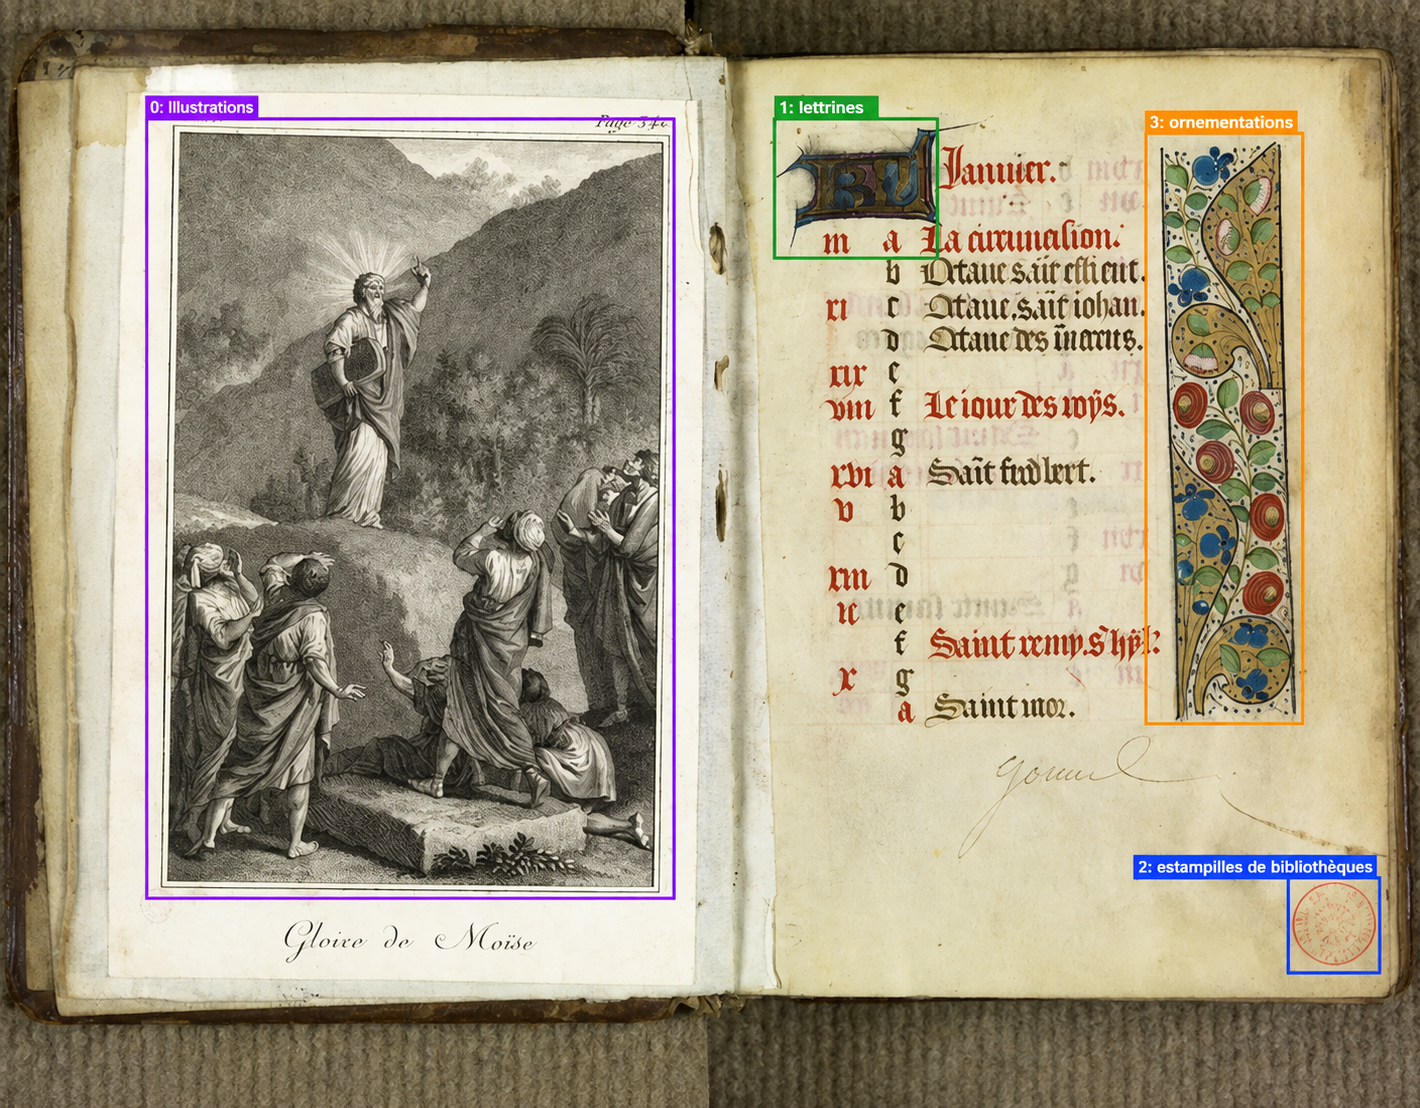
\includegraphics[height=6cm]{img/chatgpt2.png}
		\caption{Tache de détection multiclasse sur une image du jeu Horae. Ici le modèle se débrouille très bien et est proche de la qualité d'un annotateur humain.}
	\end{subfigure}
\end{figure}

\begin{figure}[h]
	\centering
	\caption{résultats pour \textit{Gemini Flash}}
	\begin{subfigure}{0.45\textwidth}
		\centering
		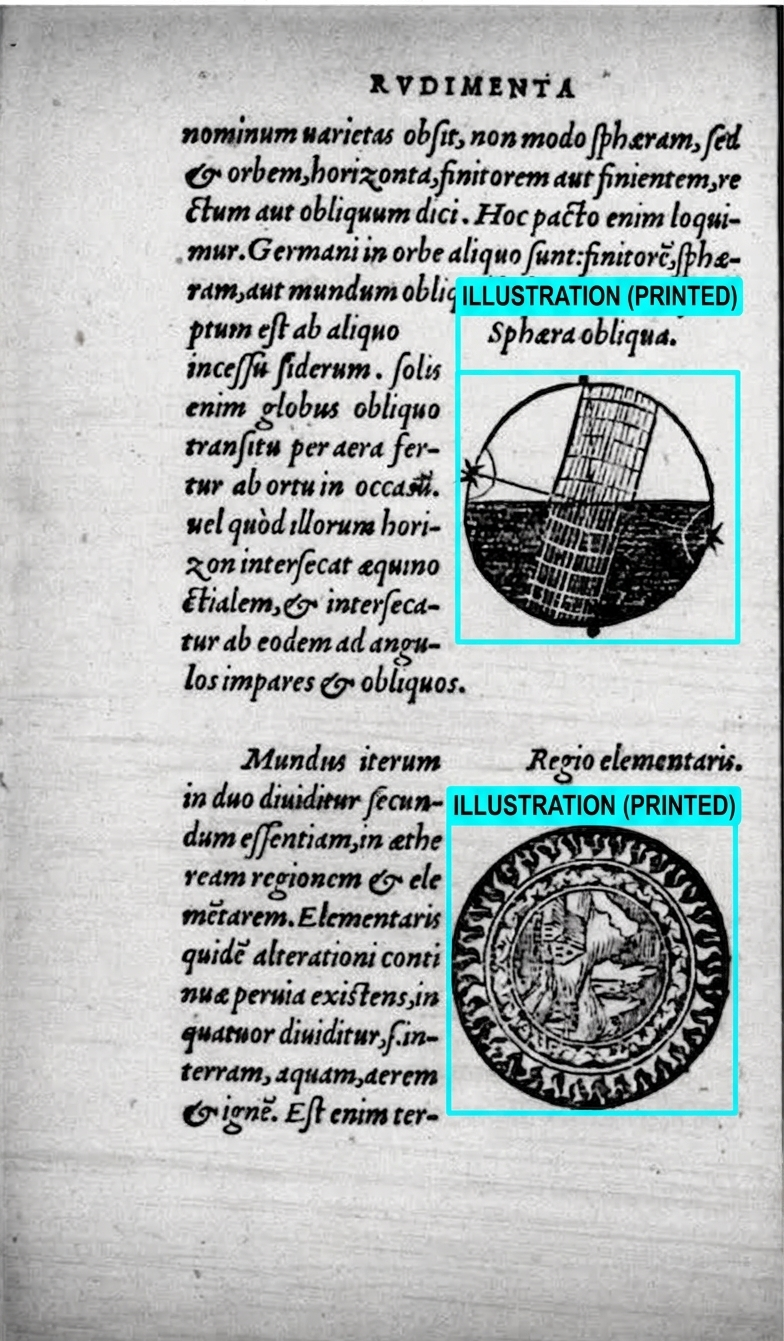
\includegraphics[height=5.5cm]{img/geminitest1.jpeg}
		\caption{Tache de détection d'illustration sur une image du jeu S-VED}
		
	\end{subfigure}
	\hfill
	\begin{subfigure}{0.45\textwidth}
		\centering
		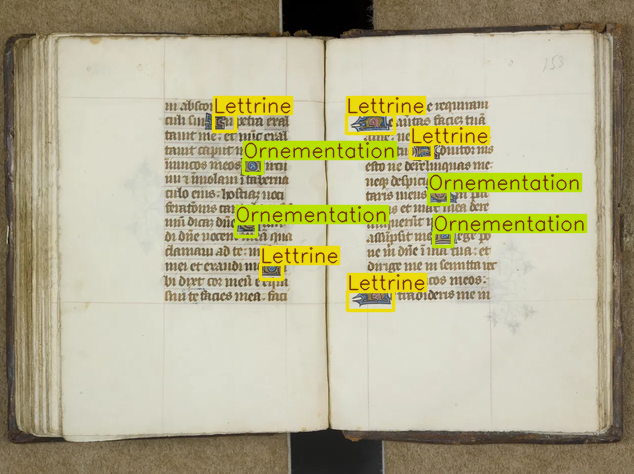
\includegraphics[height=5.5cm]{img/geminitest3.png}
		\caption{Tache de détection de lettrine sur une image du jeu Horae. Les boîtes englobantes des lettrines sont insufissantes et le modèle détecte le texte comme une illustration.}
	\end{subfigure}
	
	\begin{subfigure}{0.45\textwidth}
		\centering
		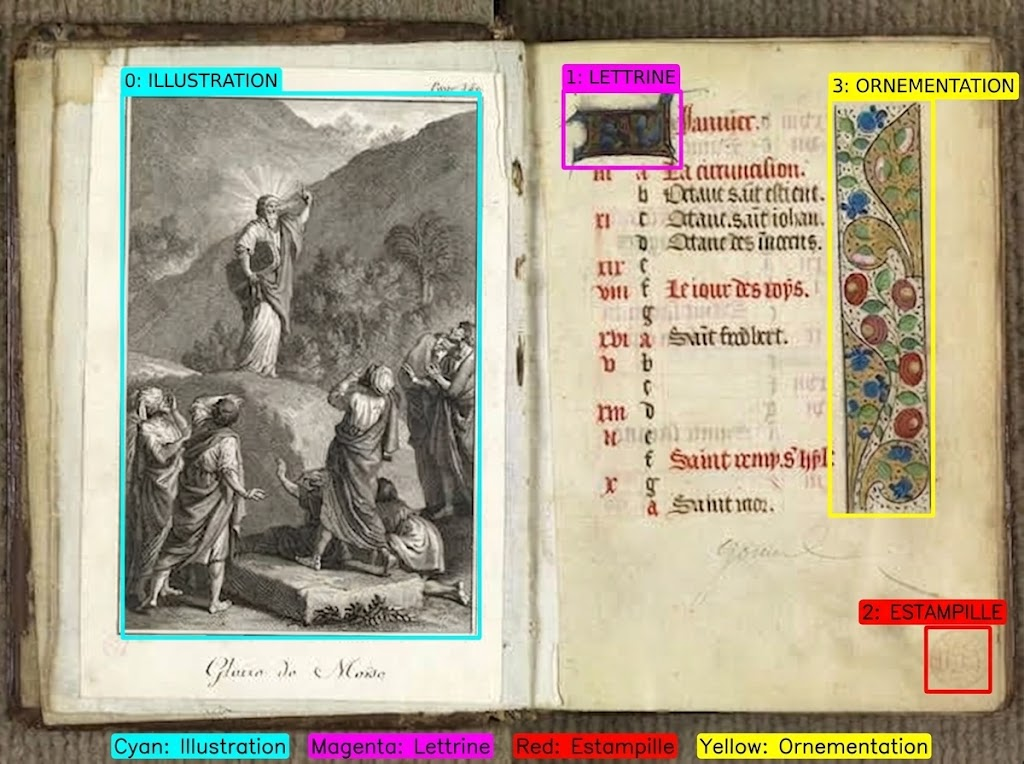
\includegraphics[height=6cm]{img/geminitest2.jpeg}
		\caption{Tache de détection multiclasse sur une image du jeu Horae. Ici le modèle se débrouille très bien et est proche de la qualité d'un annotateur humain.}
	\end{subfigure}
\end{figure}



\newpage{\pagestyle{empty}\cleardoublepage}

%%%%%%%%%%%%%%%%%%

\backmatter % glossaire, index, table des figures, table des matières.. (la bibliographie a déjà été appelée)

\printglossary[type=\acronymtype, title={Glossaire des acronymes}, style=mcolindex]

\listoffigures

\listoftables

\end{document}
